\documentclass[12pt,a4paper,openright,twoside]{report}

\usepackage[italian]{babel}
\usepackage[utf8]{inputenc}
\usepackage{fancyhdr}
\usepackage{indentfirst}
\usepackage[T1]{fontenc}
\usepackage[final]{microtype}
\usepackage{newlfont}
\usepackage{graphicx}
\usepackage{caption}
\usepackage{subcaption}
\usepackage{wrapfig}
\usepackage{minted}
\usepackage{amssymb}
\usepackage{amsmath}
\usepackage{latexsym}
\usepackage{amsthm}
\usepackage{csquotes}
\usepackage[sorting=none]{biblatex}
\usepackage[hidelinks]{hyperref}
\usepackage{silence}
\usepackage{xargs}

% \addbibresource{bibliografia/bibliografia.bib}

\hyphenation{} % vanno inserite le parole che latex non riesce a tagliare nel modo giusto andando a capo

\hypersetup{
    pdftitle={Progettazione e Implementazione di Agenti Cognitivi per Simulazioni di Evacuazioni di Folle in Alchemist}
}

% Impaginazione
\textwidth=450pt
\oddsidemargin=0pt
\linespread{1.3}
\pagestyle{fancy}
\addtolength{\headheight}{15pt}
\fancyhead[RO,LE]{\thepage}
\fancyhead[RE]{\small{\it{PROGETTAZIONE E IMPLEMENTAZIONE DI AGENTI COGNITIVI\\PER SIMULAZIONI DI EVACUAZIONI DI FOLLE IN ALCHEMIST}}}
\fancyfoot{}
% SHORTCUTS

% corsivo
\renewcommandx{\i}[1]{\emph{#1}}

% grassetto
\renewcommandx{\b}[1]{\textbf{#1}}

% nota a pie' di pagina
\newcommandx{\n}[2][1 = ]{\ifstrequal{#1}{}{%
        \footnote{#2.}%
    }{
        \footnote{\label{note:#1}#2.}%
    }%
}

% citazione
\renewcommandx{\c}[2][1 = ]{\ifstrequal{#1}{}{
        \cite{#2}%
    }{
        \cite[#1]{#2}%
    }%
}

% fra parentesi
\newcommandx{\p}[2][1 = ]{--- #2\ifstrequal{#1}{e}{}{ ---}}

% capitolo
\renewcommandx{\cap}[3][1 = ]{\ifstrequal{#1}{*}{%
        \chapter*{#2}\label{cap:#3}%
        \addcontent{#2}%
    }{%
        \chapter{#2}\label{cap:#3}%
    }
}

% sezione
\renewcommandx{\sec}[2]{\section{#1}\label{sec:#2}}

% sottosezione
\newcommandx{\sub}[2]{\subsection{#1}\label{sub:#2}}

% sottosottosezione
\newcommandx{\subsub}[2]{\subsubsection{#1}\label{subsub:#2}}

% IMPORT E CAPTIONS

% documento
\newcommandx{\doc}[1]{\input{capitoli/#1.tex}}

% immagine
\newcommandx{\img}[2][1 = 1.0]{
    \includegraphics[width=#1\linewidth]{immagini/#2}
}

% figura
\newcommandx{\fig}[7][1 = 1.0, 2 = !htb, 3 = \centering, 7 = , usedefault]{
    \begin{figure}[#2]
        #3
        \img[#1]{#4}%
        \caption{#6.}%
        \ifstrequal{#7}{}{}{(fonte: \url{#7})}%
        \label{fig:#5}%
    \end{figure}
}

% figura allineata
\newcommandx{\wfig}[8][1 = 0.5, 2 = 0.9, 3 = r, 4 = \centering, 8 = , usedefault]{
    \begin{wrapfigure}{#3}{#1\linewidth}
        #4
        \img[#2]{#5}
        \caption{#7.}
        \ifstrequal{#8}{}{}{(fonte: \url{#8})}
        \label{fig:#6}
    \end{wrapfigure}
}

% ALTRO

% aggiunta all'indice
\newcommandx{\addcontent}[1]{\addcontentsline{toc}{chapter}{#1}}

% nuova pagina
\newcommandx{\page}[1]{\clearpage{\pagestyle{#1}\cleardoublepage}}


\addbibresource{bibliografia/bibliografia.bib}

% Impaginazione
\textwidth=450pt
\oddsidemargin=0pt
\linespread{1.3}
\pagestyle{fancy}
\addtolength{\headheight}{15pt}
\fancyhead[RO,LE]{\thepage}
\fancyhead[RE]{\small{\it{PROGETTAZIONE E IMPLEMENTAZIONE DI AGENTI COGNITIVI\\PER SIMULAZIONI DI EVACUAZIONI DI FOLLE IN ALCHEMIST}}}
\fancyfoot{}

\begin{document}
\title{Progettazione e Implementazione di Agenti Cognitivi per Simulazioni di Evacuazioni di Folle in Alchemist}
\author{Diego Mazzieri}
\date{\today}

% Frontespizio
\begin{titlepage}
% INTESTAZIONE
\begin{center}
{{\Large{\textsc{Alma Mater Studiorum $\cdot$ Università di Bologna\\\vspace{2mm}Campus di Cesena}}}}
\rule[0.1cm]{15.8cm}{0.1mm}
\rule[0.5cm]{15.8cm}{0.5mm}
{\small{\bf{SCUOLA DI SCIENZE\\Corso di Laurea in Ingegneria e Scienze Informatiche}}}
\end{center}

\vspace{10mm}

% TITOLO
\begin{center}
{\Large{\bf PROGETTAZIONE E IMPLEMENTAZIONE DI}}\\
\vspace{2mm}
{\Large{\bf AGENTI COGNITIVI PER SIMULAZIONI}}\\
\vspace{2mm}
{\Large{\bf DI EVACUAZIONI DI FOLLE IN ALCHEMIST}}\\
\end{center}

\vspace{8mm}

% ELABORATO
\begin{center}
{\large{{\it Elaborato in}\\\vspace{1mm}PROGRAMMAZIONE AD OGGETTI}}
\end{center}

\vspace{22mm}

\noindent
% CREDITI
\begin{minipage}[t]{0.47\textwidth}
{\large{{\it Relatore}\\Prof. MIRKO VIROLI\\\vspace{1mm}\\{\it Correlatore}\\Prof. DANILO PIANINI}}
\end{minipage}
\hfill
\begin{minipage}[t]{0.47\textwidth}\raggedleft
{\large{{\it Presentata da}\\{DIEGO MAZZIERI}}}
\end{minipage}

\vspace{20mm}

%SESSIONE
\begin{center}
\rule[0.1cm]{15.8cm}{0.1mm}
{\large{Seconda Sessione di Laurea\\Anno Accademico 2018-2019}}
\end{center}
\end{titlepage}
\page{empty}

% Prefazione
\pagenumbering{roman}
\oddsidemargin=0pt
\evensidemargin=0pt

% Dedica
\begin{titlepage}
\doc{dedica}
\page{empty}
\end{titlepage}

\chapter*{Introduzione}
\addcontentsline{toc}{chapter}{Introduzione}
Le vicende di piazza San Carlo a Torino e della discoteca \enquote{Lanterna Azzurra} di Corinaldo sono solo degli esempi a noi vicini geograficamente e cronologicamente di come l'evacuazione di una folla possa sfociare in una tragedia se non si considerano adeguatamente: l'afflusso, i potenziali pericoli e il comportamento dei partecipanti. \newline
La simulazione computerizzata rappresenta uno dei più potenti strumenti a disposizione dell'uomo per prevenire questo genere di situazioni, evitando errori che possono irrompere in una vastissima quantità di casistiche, dall'organizzazione di un evento alla costruzione di un edificio. \newline
Gli ultimi trent'anni hanno visto la nascita di moltissimi modelli che, pur derivando la loro formulazione da teorie molto diverse, perseguono tutti il medesimo scopo di riprodurre le azioni di un notevole numero di persone. Tra le varie metodologie di simulazione presenti, quella basata sugli agenti, esseri autonomi in grado di interagire tra loro, è stata scelta come punto di partenza, data la sua flessibilità e naturalezza nel descrivere un sistema costituito da molte componenti differenti come quello in esame. \newline
Mentre notevoli sviluppi sono stati conseguiti in merito alla descrizione delle varie forze fisiche in gioco, meno esplorati sono i temi relativi alle capacità cognitive e relazionali delle persone. \newline 
Tali aspetti sono essenziali da considerare per ambire ad un risultato realistico e non possono essere trascurati nello studio del comportamento di una folla, soprattutto nei casi di emergenza, dove la loro importanza è ulteriormente amplificata. É in queste occasioni, infatti, che fenomeni quali la trasmissione del panico e l'appartenenza ad un gruppo costituiscono le principali cause delle decisioni prese da ogni individuo. \newline
Focalizzando l'attenzione su questi concetti, il lavoro di tesi qui presentato ha come obiettivo quello di inserire all'interno del simulatore stocastico Alchemist gli elementi caratterizzanti l'evacuazione di una folla in una accezione generale, senza concentrarsi su nessuno scenario specifico, in modo da fornire gli strumenti necessari per ricreare svariate situazioni di interesse. \newline
Il ruolo di agente della simulazione è assunto da ogni singolo pedone; di conseguenza, parte integrante del progetto è stata quella di attribuire ad esso la facoltà di muoversi all'interno dell'ambiente considerando la combinazione di diverse azioni e seguendo delle precise strategie, al fine di ottenere uno steering realistico. \newline
I risultati attualmente raggiungibili permettono di apprezzare la rilevanza dei vari fattori analizzati, ma quella che si ha di fronte durante il decorrere della simulazione è ancora una modesta approssimazione della realtà. \newline
La trattazione è stata articolata in quattro capitoli. Nel primo viene fatta una panoramica sul problema del comportamento delle folle discutendo le teorie socio-psicologiche su cui esso si basa, gli avvenimenti tragici che purtroppo l'hanno contraddistinto e i vari approcci presenti in letteratura per affrontarlo. \newline
Nel secondo capitolo vengono spiegate le scelte effettuate in fase di analisi, progettazione e implementazione, per definire le varie entità introdotte compatibilmente con la struttura e in relazione al meta-modello alla base di Alchemist.
Nel terzo capitolo sono raccolti alcuni esempi di simulazione, ognuno dei quali concerne un fenomeno particolarmente significativo nell'ambito dell'evacuazione di folle. \newline
Nel quarto capitolo, infine, si traggono le conclusioni sui contributi offerti da questo lavoro e si consigliano delle possibili direzioni di sviluppo future con cui è possibile ampliarlo.
\page{empty}

% Indice
\tableofcontents
\page{empty}

% Capitoli
\pagenumbering{arabic}

\chapter{Background}
\section{Il comportamento delle folle}
Lo studio del comportamento collettivo è un ambito sociologico che fonda le proprie radici nelle ricerche dell'antropologo e sociologo francese Gustave Le Bon, autore del libro \enquote{Psicologia delle folle} \cite{Bon1895} pubblicato nel 1895, nel quale egli analizza come l'appartenenza di un individuo ad una conformazione come quella della folla possa inconsciamente causare in esso un attenuamento delle proprie capacità critiche, dovuto alla tendenza a conformarsi alle decisioni scaturite ed alimentate dall'istinto collettivo. Questa \i{teoria del contagio}, come la definisce Le Bon stesso, porta ogni individuo a giustificare le proprie azioni identificandosi non più come singolo, ma come parte costitutiva della folla. \newline
Per spiegare le cause di questo fenomeno Ralph Turner e Lewis Killian, durante la seconda metà degli anni '50, formularono la \i{teoria della norma emergente} \cite{Turner1957}, sottolineando come le decisioni di un ristretto numero di persone all'interno della folla, siano accettate dal resto degli appartenenti ad essa perché i processi di interazione creano involontariamente degli obiettivi comuni che rafforzano determinate scelte inibendone altre, anche se queste avrebbero rispecchiato maggiormente la volontà del singolo individuo. \newline
È un fenomeno quanto mai attuale e tangibile che può essere riscontrato anche quando le persone, non essendo compresenti, non sono fisicamente influenzabili una con l'altra, ma subiscono questo meccanismo tramite l'azione dei mass media e di Internet, come dimostra in maniera eclatante lo scandalo di Cambridge Analytica\n{\url{https://web.archive.org/web/20190911084718/https://www.ilpost.it/2018/03/19/facebook-cambridge-analytica/}}. \newline
Quando questo avviene in presenza di una grande quantità di persone concentrate in uno spazio ristretto, però, le conseguenze possono essere catastrofiche anche se in risposta ad un apparentemente insignificante azione localizzata, che rischia di scatenare una reazione a catena e generare una situazione incontrollabile. \newline
La tendenza a riunirsi per condividere passioni, organizzare manifestazioni, o visitare luoghi di interesse è da sempre un elemento caratteristico dell'uomo e molto probabilmente continuerà sempre ad esserlo; riuscire a prevedere il comportamento delle folle presenti in queste occasioni è perciò di fondamentale importanza.

\subsection{L'evacuazione delle folle}
Una situazione in cui è particolarmente difficile studiare il comportamento di una folla è quella dell'evacuazione. Infatti, se la tendenza a conformarsi alle dinamiche collettive è un istinto naturale di ogni individuo in condizioni normali, nelle situazioni di emergenza, dove a causa di un pericolo imminente entrano in gioco fattori come il panico e il nervosismo, una persona modifica le proprie capacità logiche e decisionali \cite{Helbing2011}. \newline 
Le reazioni si manifestano sia fisicamente, ad esempio con l'aumento della propria velocità, sia psicologicamente, con l'attitudine ad affidarsi e ad emulare gli altri elementi della folla, senza riuscire a realizzare che probabilmente anche loro si trovano nella medesima situazione di non lucidità. Quello che ne deriva è un comportamento non coordinato e svantaggioso per l'obiettivo finale, che per le sua somiglianza con il mondo animale viene definito \enquote{effetto gregge}. La figura \ref{fig:herding} illustra le possibili conseguenze che da esso  potrebbero scaturire. \newline
Riuscire a controllare questi atteggiamenti comporterebbe sicuramente un netto miglioramento dei tempi necessari per la buona riuscita dell'evacuazione; tuttavia è irrealistico pensare di poter obbligare una persona ad agire seguendo uno schema premeditato in una situazione caratterizzata da un forte stress emotivo. \newline
Piuttosto, è doveroso prendere in considerazione anche questi comportamenti, per provare ad analizzare approfonditamente lo scenario di interesse e prevedere come decorreranno i fatti.

\fig[0.75]{herding-behavior.png}{herding}{Illustrazione dell'\enquote{effetto gregge} durante l'evacuazione da una stanza che presenta due uscite}

\subsubsection{Evacuazione da edifici o imbarcazioni}
Uno dei settori in cui il tema dell'evacuazione è di primaria importanza è senza dubbio quello della costruzione di strutture destinate ad ospitare molte persone. Durante la progettazione di un edificio o di una imbarcazione, infatti, ci sono molti fattori che devono essere tenuti in considerazione per ridurre i tempi necessari a permettere ai presenti di lasciare in sicurezza il fabbricato. \newline 
Le principali scelte vertono sul posizionamento e la dimensione delle uscite, ma anche sul dislocamento dei diversi oggetti che, per scopi logistici o di arredamento, devono essere presenti nell'ambiente che si sta progettando e che, in sede di evacuazione, rappresentano degli ostacoli che impediscono di raggiungere lo spazio esterno il prima possibile. \newline
Anche se apparentemente semplici, queste decisioni possono spesso nascondere delle insidie che intuitivamente non riusciamo ad interpretare come tali. \newline 
La presenza di un'uscita più grande e visibile delle altre, ad esempio, può sembrare una buona strategia per avere sempre un punto di riferimento con cui orientarsi mentre, in realtà, può trasformarsi in un fattore limitante, in grado di favorire il già menzionato comportamento del gregge, nel momento in cui tutti i presenti, avendo come unico obiettivo quello di scappare, sono involontariamente portati ad andarvi incontro ignorando la presenza delle altre \cite{Almeida2013}. \newline
Al contempo, ci sono delle soluzioni apparentemente pessime che, in realtà, si dimostrano ottime alla prova dei fatti. Un esempio lampante è quello della presenza di una colonna davanti ad un'uscita, che costringendo la folla a dividersi in due gruppi, diminuirebbe la pressione proveniente dal retro e abbasserebbe i tempi di deflusso di oltre il 50\% \cite{Helbing2002}. Paradossalmente, è proprio per questa sua natura contro-intuitiva e per la falsa percezione di pericolo che susciterebbe, che questo espediente non viene quasi mai adottato. \newline
Un'altra interessante idea progettuale è quella della costruzione di corridoi non rettilinei ma a zigzag, che, in caso di una alta pressione, sono adatti a distribuire in più direzioni la spinta dei pedoni \cite{Helbing2005}.

\subsection{Eventi rilevanti}
L'urgenza di dover attuare delle contromisure al fine di perseguire una gestione controllata del comportamento di una folla, è evidenziata dall'ingente numero di incidenti e disastri a cui l'umanità ha assistito nel corso della sua storia. Solo tra il 1971 e il 2011 è possibile elencarne ben 156 \cite{Soomaroo2012} e questo tipo di situazione è destinato a diventare sempre più frequente, poiché la visibilità ed il raggiungimento del luogo in cui si trova l'evento sono obiettivi sempre più facili da conseguire.

\paragraph{La strage di Hillsborough}
Tra i maggiori palchi scenici che fanno da cornice a questi tragici scenari e che vedono la folla come protagonista, non si possono non menzionare gli stadi calcistici. \newline 
L'esempio più tragico facente parte di questa categoria è quello dell'Hillsborough Stadium di Sheffield il 15 aprile del 1989, che ha visto ben 96 morti e oltre 400 feriti a causa della sottostima del numero di spettatori appartenenti alle due tifoserie rivali\n{\url{https://time.com/4836782/hillsborough-disaster-history-charges/}}. \newline 
Le entrate previste, infatti, non erano idonee alla mole di persone accorse. Per provare a rimediare alla situazione, la polizia pensò di aprire anche l'ingresso che conduceva direttamente al settore centrale della curva, credendo in questo modo di evitare che si creassero disordini negli ingressi predisposti. Quello che ne scaturì, invece, fu un disastro irrimediabile; tutti coloro che erano ancora al di fuori dello stadio, intuendo la presenza di una via per arrivare in tempo, si riversarono all'interno di essa e raggiunsero gli spalti, dove, a causa della mancanza di spazio, i tifosi già presenti furono costretti a provare a scavalcare le recinzioni o a rimanere schiacciati e soffocati, come testimonia la foto in figura \ref{fig:hillsborough}.

\fig[0.8]{hillsborough.jpg}{hillsborough}{Tifosi schiacciati contro le recinzioni dal sovraffollamento}[www.time.com]

\paragraph{I pellegrinaggi alla Mecca}
Ancora più preoccupante è il caso del pellegrinaggio alla Mecca, dove il problema dell'altissima densità di persone si ripresenta costantemente. Nonostante questo cammino sia uno dei cinque pilastri della religione islamica, che ogni anno coinvolge più di due milioni di fedeli, sono più di 5000 le persone che hanno perso la vita per motivi inerenti al sovraffollamento\n{\url{https://en.wikipedia.org/wiki/Incidents\_during\_the\_Hajj}}. \newline
Nell'anno 2015 in particolare, il numero delle vittime ha per la prima volta superato i 2000 individui, anche se le circostanze dell'evento non sono ancora ufficialmente chiarite. Dalle dichiarazioni dei sopravvissuti\n{\url{https://web.archive.org/web/20190810075436/https://www.nytimes.com/interactive/2016/09/06/world/middleeast/2015-hajj-stampede.html}}, trapela che le ragioni del disastro siano imputate all'impatto tra due flussi di fedeli, confluiti all'interno della stessa strada in prossimità del ponte Jamarat (figura \ref{fig:hajj}). Un ingente gruppo ha dovuto intraprendere una deviazione a causa dell'interruzione di una delle rotte predefinite e nel momento in cui la massa si è riversata su un tratto destinato ad un altro gruppo, si è generata un'altissima pressione tra i presenti.

\fig[0.8]{hajj.jpg}{hajj}{Fedeli presenti sul ponte Jamarat per il rituale della \enquote{lapidazione del diavolo}}[www.bbc.com]

\paragraph{Le tragedie di piazza San Carlo e di Corinaldo}
Senza dover andare troppo lontano né geograficamente né temporalmente, è doveroso ricordare anche le tragedie di piazza San Carlo a Torino (3 giugno 2017), in occasione della proiezione della finale di Champions League, e della discoteca \enquote{Lanterna Azzurra} di Corinaldo (8 dicembre 2018), in cui era progrmmato il concerto del rapper \i{Sfera Ebbasta}. \newline
In entrambe le occasioni, l'utilizzo di spray urticante ha generato il panico tra i presenti. Nel primo caso, sono stati oltre 30000 i partecipanti e il tentativo di fuga di gran parte di essi, ha portato alla morte di due persone e ad oltre 1500 feriti; nel secondo, il parapetto ha ceduto a causa dell'ingente numero di persone presenti, causando la caduta di svariate decine di spettatori e provocando 6 decessi.

\subsection{Il divario tra simulazione e realtà}
Le procedure di esercitazione all'evacuazione, pensate allo scopo di verificare l'efficacia delle procedure di sicurezza in caso di emergenza, non sono sempre attuabili. Tale limitazione è dovuta al fatto che, tralasciando le difficoltà organizzative e gli ingenti costi dell'operazione in casi analoghi a quelli sopra citati, sarebbe necessario esporre le persone ai reali pericoli che potrebbero insorgere nell'ambiente. \newline 
Effettuare delle simulazioni solamente ipotizzando il potenziale pericolo, come avviene in quelle a cui tutti abbiamo partecipato almeno una volta a scuola o in un luogo di lavoro, si riduce spesso ad una formalità o addirittura ad un momento di svago, che raramente rispecchia le reazioni che i medesimi protagonisti avrebbero nel caso l'emergenza diventasse reale. \newline
Al fine di realizzare predizioni, quello di cui ci si potrebbe munire è uno strumento che non implichi eventuali rischi nell'utilizzo, sia facilmente adattabile in risposta ai cambiamenti, e permetta la valutazione nel minor tempo possibile del maggior numero di scenari di interesse. \newline
Uno strumento capace di sintetizzare insieme tutti questi requisiti è quello della simulazione computerizzata che, negli ultimi 30 anni, ha rappresentato un'importante risorsa per le nuove scoperte conseguite in questo ambito di ricerca.
\section{La simulazione computerizzata}
Per riuscire ad orientarsi nel vasto panorama dei modelli esistenti inerenti il problema dell'evacuazione di folle, è necessario innanzitutto capire quali sono i principali criteri secondo cui ognuno di essi può essere classificato. \newline
La prima grande separazione può essere effettuata definendo le categorie \textit{macroscopico} e \textit{microscopico}, infatti, mentre un modello macroscopico non è costruito a partire dal pedone ma simula il comportamento dell'intera folla come un'unica entità, un modello microscopico analizza le azioni delle singole persone a livello locale e, dai loro apporti individuali, determina il movimento globale della folla. \newline
Un'altra differenziazione riguarda le modalità con cui vengono gestiti spazio e tempo all'interno dell'ambiente di simulazione. Specificatamente, la scelta verte tra l'opzione computazionalmente più vantaggiosa del \textit{discreto} e quella del \textit{continuo}, sovente più fedele alla realtà da simulare. \newline
Mentre i modelli macroscopici considerano i pedoni come tutti uguali tra loro, vista l'impossibilità di analizzare il singolo individuo, i modelli di tipo microscopico possono differenziarsi in \textit{eterogenei} ed \textit{omogenei}, per enfatizzare la possibilità o meno di rappresentare all'interno della folla persone che presentano caratteristiche distinte.

\subsection{Approcci esistenti}
Analizzando i principali modelli di simulazione delle folle presenti allo stato dell'arte \cite{Duives2013} \cite{Zheng2009}, è possibile individuare delle analogie nelle metodologie con cui questi sono stati formulati. In particolare, è possibile identificare quattro distinte tipologie di approccio, le cui principali caratteristiche sono riassunte nella tabella \ref{table:models-comparison}. 

\begin{table}
\centering
\renewcommand{\arraystretch}{1.5}
\begin{tabular}{|c|c|c|c|}
\hline
\textbf{Modello}            & \textbf{Tipologia} & \textbf{Spazio e Tempo} & \textbf{Pedone} \\ \hline
\textbf{Automi cellulari}   & Microscopico       & Discreto                & Omogeneo        \\ \hline
\textbf{Forze sociali}      & Microscopico       & Continuo                & Eterogeneo      \\ \hline
\textbf{Basati sull'agente} & Microscopico       & Discreto/Continuo       & Eterogeneo      \\ \hline
\textbf{Fluidodinamici}     & Macroscopico       & Continuo                & Omogeneo        \\ \hline
\end{tabular}
\caption{Tabella comparativa delle tipologie di modello di evacuazione di folle.}
\label{table:models-comparison}
\end{table}

\subsubsection{Automi cellulari}
Un automa cellulare è un sistema dinamico discreto, in cui lo spazio è rappresentato mediante una griglia di celle mentre il tempo da intervalli temporali prestabiliti. \newline
A partire da una configurazione in cui il sistema si trova ad una determinata iterazione, è possibile ottenere la successiva applicando l'insieme di regole costitutive del modello. Una regola ha lo scopo di modificare lo stato di ogni cella della griglia in relazione allo stato di quelle ad essa adiacenti. \newline
Nel caso dell'evacuazione di una folla, ad esempio, è possibile rappresentare i pedoni come celle oscurate e definirne il movimento tramite lo spostamento in una delle otto posizioni ad essa adiacenti, considerando l'eventuale presenza di altri pedoni e la vicinanza all'uscita. \newline
La semplicità concettuale che caratterizza questo tipo di modelli li rende sia computazionalmente molto efficienti sia adatti ad analizzare l'evoluzione di varie categorie di sistemi, da quelli biologici a quelli fisici. \newline
L'approssimazione di una qualsiasi entità con una cella però, in molte situazioni può risultare troppo riduttiva e poco descrittiva del problema in esame.

\subsubsection{Forze sociali}
Proposto per la prima volta da D. Helbing e P. Molnar \cite{Helbing1995}, il modello forze sociali si basa sull'assunzione che il movimento dei pedoni, apparentemente visto come un processo caotico, è il risultato dell'apporto di diversi fattori quali: la volontà di raggiungere una destinazione, mantenere una distanza da eventuali ostacoli o essere attratti dagli altri individui presenti. \newline 
Ognuno di questi stimoli, chiamati appunto \i{forze sociali}, susciterebbe nel pedone delle diverse reazioni, dipendenti dalle intenzioni di ognuno a compiere una piuttosto che l'altra azione e la cui combinazione determina la velocità e la direzione del movimento in ogni istante.

\subsubsection{Ad agenti}
I modelli basati sugli agenti approssimano il sistema con un insieme di entità capaci di interagire con i propri simili e di prendere delle decisioni autonome sulla base di un insieme di regole. \newline
Ogni agente ha il proprio stato interno, che può variare nel corso della simulazione in risposta a determinati eventi e lo rende riconoscibile rispetto a tutti gli altri. Le sue capacità relazionali, inoltre, permettono l'emergere di fenomeni che non si riscontrerebbero valutando separatamente il comportamento dei singoli. \newline 
Per queste loro caratteristiche, i modelli ad agenti si rivelano particolarmente flessibili ad essere arricchiti con nuovi livelli di dettaglio, grazie ai quali è possibile avvicinarsi sempre più ad una simulazione fedele alla realtà. \newline
Spesso, il loro principale limite, risiede nella difficoltà a scalare verso l'alto il numero di agenti presenti nella simulazione.

\subsubsection{Fluidodinamici}
A differenza dei precedenti, i modelli fluidodinamici sono di tipo macroscopico e si basano sull'assunzione che il movimento della folla è molto simile allo scorrimento di un fluido. \newline
Come sottolineato da Hughes \cite{Hughes2002}, questa formulazione, per essere considerata attendibile, richiede una densità di pedoni molto alta, altrimenti non si potrebbe giustificare l'uso delle equazioni di Navier-Stokes\n{\url{http://web.archive.org/web/20190522071242/https://www.comsol.it/multiphysics/navier-stokes-equations}}, le cui ipotesi sono quelle di modellare un continuo deformabile. \newline
L'utilizzo di questo tipo di approccio si rileva molto utile in casi analoghi al sopracitato pellegrinaggio alla Mecca, dove l'elevatissimo numero di presenti rende proibitivo l'impiego degli altri modelli. \newline
L'aspetto limitante risiede nel fatto che la precisione dei modelli fluidodinamici è vincolata alla quantità di pedoni presenti nella folla, che, se non sufficientemente alto, comporta una approssimazione troppo grossolana.

\subsection{Il modello IMPACT}
Il problema della maggior parte dei modelli esistenti è che essi rivolgono la loro attenzione principalmente sulle leggi fisiche e le forze in gioco nella simulazione, considerando i pedoni come particelle invece che come entità con caratteristiche socio-culturali peculiari ed una componente emotiva facilmente influenzabile da quella dei propri vicini \cite{Zheng2009}. \newline
Il modello ad agenti IMPACT \cite{vanderWal2017Model} nasce con l’obiettivo di analizzare l'importanza di questi aspetti, che vengono valutati all'interno di simulazioni inerenti l'evacuazione a causa di un incendio da un hub di trasporto.

\subsubsection{Network Oriented Modeling}
Per definire l'evoluzione dei processi emotivi dei pedoni viene usato l'approccio del Network Oriented Modeling \cite{Treur2018}. Questa scelta permette di descrivere attraverso un grafo orientato processi interconnessi tra loro e viene utilizzata nei più svariati ambiti, dalla biologia alla sociologia. \newline 
Ogni caratteristica che si desidera rappresentare costituisce un nodo del grafo, il cui stato $y(t)$ varia nel tempo secondo la seguente equazione differenziale:

\begin{equation*}
    \frac{dy(t)}{dt} = \eta_{y}[c_{y}(w_{x_1,y} \cdot x_1(t),...,w_{x_k,y} \cdot x_k(t)) - y(t)]
\end{equation*}

che in versione discreta può essere riscritta come

\begin{equation*}
    y(t + \Delta t) = y(t) + \eta_{y}[c_{y}(w_{x_1,y} \cdot x_1(t),...,w_{x_k,y} \cdot x_k(t)) - y(t)]\Delta t
\end{equation*}

dove $\eta_{y}$ è un fattore moltiplicativo utile a regolare la velocità dell'evoluzione, le $x_i(t)$ sono gli stati dei processi che influenzano l'aggiornamento di $y(t)$ e $c_{y}$ é la funzione che decide come devono essere combinati i vari $x_i(t)$ moltiplicati per i rispettivi pesi $w_{i,y}$.

\begin{figure}[ht]
  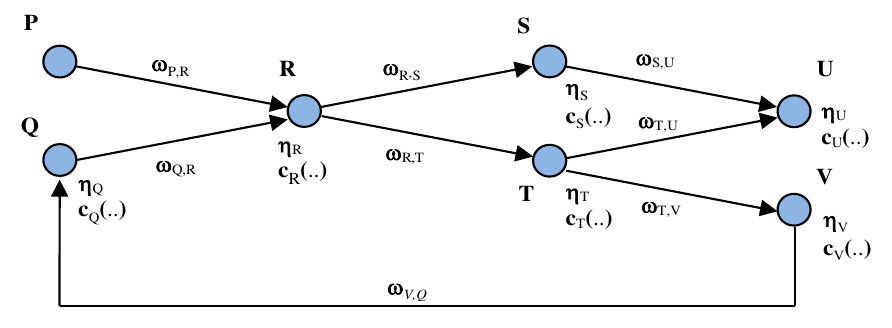
\includegraphics[width=\linewidth]{immagini/network-oriented-modeling.png}
  \caption{Esempio di Network Oriented Modeling rappresentato mediante grafo: i nodi contrassegnati con le lettere da P a V sono gli stati dei processi presi in considerazione, che vengono aggiornati valutando la provenienza e i pesi $w_{P..V,P..V}$ degli archi entranti utilizzando la rispettiva funzione di combinazione $c_{P..V}$.}

  \label{fig:net-model}
\end{figure}

\subsubsection{Risultati delle simulazioni}
Per determinare il reale impatto dei vari fattori presi in considerazione è stato utilizzato, come ambiente rappresentante un hub di trasporto, uno spazio quadrato di lato $20m$ con un'uscita in corrispondenza ad ognuno dei quattro muri ed un incendio nelle vicinanze del centro. Tale scelta, piuttosto semplice, ha l'obiettivo di ridurre al minimo il rischio che eventuali motivi strutturali, possano compromettere l'analisi della rilevanza delle caratteristiche descritte nel modello, che invece, in questo modo, rappresentano la principale fonte di variabilità all'interno della simulazione. \newline
Tra i vari aspetti presi in considerazione, il contagio sociale, fenomeno psicologico che porta al diffondersi di comportamenti, atteggiamenti o convinzioni comuni tra persone a contatto tra loro, si è dimostrato uno dei fattori più importanti, in grado di diminuire di circa il 20\% il tempo di evacuazione rispetto a quando non considerato nella simulazione, grazie alla capacità di instillare nei presenti la necessità di fuggire senza che essi avessero concretamente percepito il pericolo \cite{vanderWal2017Simulations}.

\subsubsection{Limitazioni}

\paragraph{Specificità} 
Pur presentando interessanti idee dal punto di vista sociologico e matematico, l'unico scenario analizzato nelle simulazioni di evacuazione è quello di un incendio in un hub di trasporto. Sarebbe utile riuscire a riutilizzare il medesimo modello di pedone anche all'interno di altri scenari di simulazione e in altri simulatori.

\paragraph{Movimento}
Mentre molta attenzione è posta sull'aspetto cognitivo e interazionale del pedone all'interno della folla, poco viene analizzata la parte inerente al movimento per raggiungere l'uscita che, per essere considerato realistico, non dovrebbe sia non permettere la sovrapposizione dei pedoni sia tenere in considerazione la presenza di eventuali ostacoli all'interno dell'ambiente da evacuare.

\paragraph{Implementazione}
L'utilizzo in fase di implementazione del linguaggio multi-agente NetLogo rende obbligatorio l'impiego dell'omonimo IDE per l'esecuzione delle simulazioni, che vincola lo spazio in cui si muovono gli agenti a non poter essere modellato in maniera continua. \newline 
Inoltre, tutto il codice inerente il modello è contenuto in un unico file da più di 6000 righe di codice, che risulta di difficile interpretazione. Poter mettere in pratica i principi della programmazione orientata agli oggetti e sfruttare le potenzialità di un linguaggio di programmazione all'avanguardia, permetterebbe una più agevole manutenibilità del codice, renderebbe più immediata la risoluzione di problemi, e faciliterebbe l'estensione con nuove funzionalità dell'attuale versione.
\section{Il simulatore Alchemist}
Alchemist \cite{Pianini2013} è un simulatore stocastico nato come progetto all'interno dell'Università di Bologna, che permette la simulazione di scenari inerenti la computazione pervasiva, aggregata ed ispirata alla natura.
\newline
Alchemist si basa sull'algoritmo di simulazione stocastica (SSA) \textit{Next Reaction Method} \cite{Gibson2000} che è una versione più efficiente dell'algoritmo di Gillespie \cite{Gillespie1977}.

\subsection{Modello di dominio}
Le entità costituenti il meta-modello fondante di Alchemist, di cui viene fornita una rappresentazione grafica in figura \ref{fig:alchemist-model}, sono fortemente ispirate al mondo della chimica, come anche il nome del simulatore suggerisce:
\begin{itemize}
 \item \textbf{Molecola}: corrispettivo del concetto di variabile in un linguaggio di programmazione.
 \item \textbf{Concentrazione}: valore associato ad una particolare molecola.
 \item \textbf{Nodo}: contenitore di molecole e reazioni.
 \item \textbf{Ambiente}: esprime il concetto di spazio e contiene i nodi, gestendo la loro posizione e il loro movimento al suo interno.
 \item \textbf{Regola di collegamento}: funzione che associa ad ogni nodo un vicinato.
 \item \textbf{Vicinato}: insieme di nodi in relazione tra loro per mezzo di una regola di collegamento.
 \item \textbf{Reazione}: un qualsiasi evento che può cambiare lo stato dell'ambiente. È costituita da condizioni e azioni.
 \item \textbf{Distribuzione temporale}: funzione che esprime gli istanti temporali nei quali una reazione deve avvenire.
 \item \textbf{Condizione}: funzione che determina l'eventuale esecuzione e la frequenza delle azioni contenute in una reazione.
 \item \textbf{Azione}: cambiamento dell'ambiente che scaturisce da una reazione.
\end{itemize}
Nonostante questa natura apparentemente molto specifica, la principale caratteristica del simulatore è quella della generalità, che viene raggiunto attraverso l'uso delle \textbf{incarnazioni}, istanze concrete del meta-modello in cui ogni entità viene mappata ad un corrispettivo concetto dell'universo di interesse.
Le incarnazioni attualmente esistenti in Alchemist sono:
\begin{itemize}
 \item \textbf{Protelis}: incentrata sul linguaggio Protelis \cite{Pianini2015} e la programmazione aggregata, lo studio di dinamiche collettive a partire dall'interazione non coordinata delle singole entità.
 \item \textbf{SAPERE}: per la simulazione di scenari che traggono ispirazione da ecosistemi naturali.
 \item \textbf{Biochemistry}: utilizzata per sistemi cellulari, reazioni chimiche e più in generale per tutto il mondo della biochimica.
 \item \textbf{Scafi}: anch'essa dedicata alla programmazione aggregata ma basata sul framework scafi \cite{Casadei2016}.
\end{itemize}

\begin{figure}
  \centering
  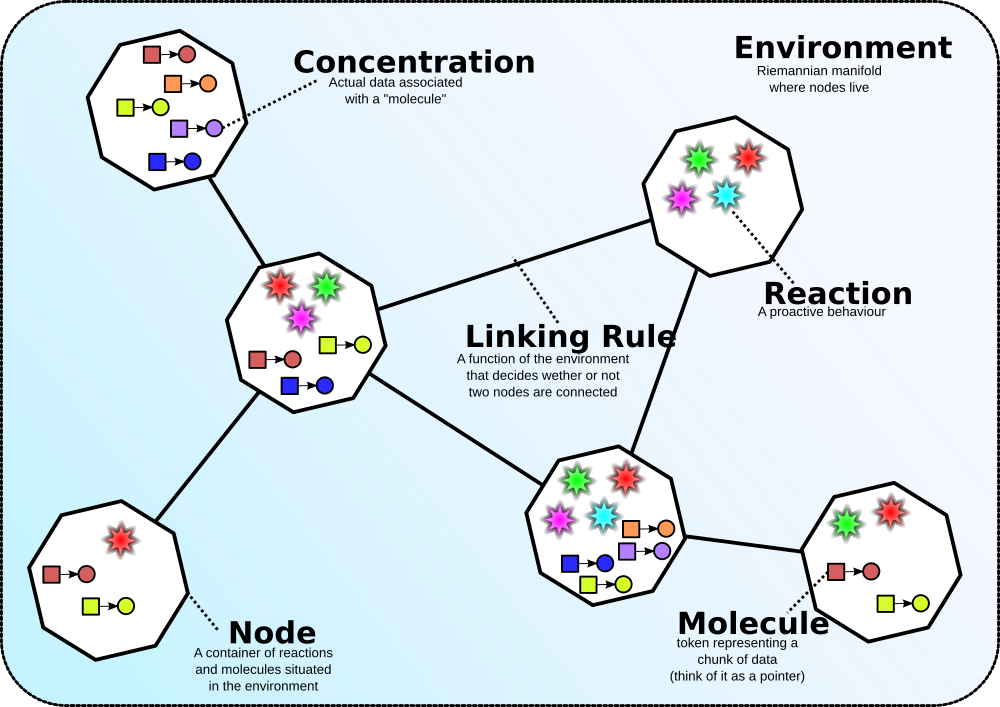
\includegraphics[width=0.80\linewidth]{immagini/alchemist-model.png}
  \caption{Il metamodello alla base di Alchemist.}
  \label{fig:alchemist-model}
\end{figure}

\subsection{Funzionalità}

\paragraph{Esecuzione batch} Al fine di poter effettuare dei confronti al variare dei parametri usati, Alchemist offre delle funzionalità batch, grazie alle quali una simulazione viene ripetuta per ogni valore nel range specificato.

\paragraph{Caricamento planimetrie} L'\texttt{ImageEnvironment} tra gli ambienti utilizzabili nelle simulazioni, permette il caricamento di una planimetria a partire da un'immagine, convertendo i pixel adiacenti del colore specificato in ostacoli.

\paragraph{Mappe geografiche} Il supporto agli standard GPX e GPS rende possibile il caricamento di mappe all'interno di  ambienti di tipo \texttt{MapEnvironment}, utili, ad esempio, in uno scenario di analisi del traffico stradale.

\paragraph{Calcolo distribuito} Considerata la possibilità di dover simulare scenari computazionalmente molto ardui da gestire, Alchemist offre il supporto ai sistemi grid, in cui il carico di lavoro viene suddiviso tra più calcolatori collegati alla medesima rete.

\subsection{Utilizzo}
Il linguaggio predefinito per la scrittura delle simulazioni in Alchemist è YAML\n{\url{https://yaml.org}}, uno standard di serializzazione dati facilmente leggibile anche dagli esseri umani. \newline
L'unico parametro da specificare obbligatoriamente per la corretta esecuzione di una simulazione è l'incarnazione da utilizzare, tutti gli altri parametri sono o indotti a partire da essa o specificati al fine di fornire ulteriori dettagli dello scenario di interesse. \newline
La principali chiavi utilizzabili all'interno di un file di simulazione Alchemist sono:
\begin{itemize}
    \item \texttt{incarnation}: l'incarnazione da utilizzare tra \texttt{protelis}, \texttt{sapere}, \texttt{biochemistry} e \texttt{scafi}.
    \item \texttt{seeds}: specifica i \textit{semi} da utilizzare per la generazione di numeri casuali. Ve ne sono solo due, \texttt{scenario} e \texttt{simulation}, impiegati rispettivamente per la creazione e l'esecuzione della simulazione.
    \item \texttt{variables}: valori che si vogliono riutilizzare all'interno del file di simulazione. Possono rappresentare sia semplici numeri che oggetti complessi come classi.
    \item \texttt{environment}: la tipologia di ambiente all'interno del quale si svolge la simulazione.
    \item \texttt{network-model}: la regola di collegamento con la quale sono associati i vari nodi.
    \item \texttt{displacements}: le posizioni in cui sono collocati i nodi all'inizio della simulazione.
    \item \texttt{layers}: gli strati rappresentanti le concentrazioni di determinate molecole in ogni punto dell'ambiente.
\end{itemize}
Per una descrizione più dettagliata delle chiavi utilizzabili si può far riferimento al sito ufficiale del simulatore\n{\url{https://alchemistsimulator.github.io/wiki/usage/yaml/}}.

\subsection{Accorgimenti}
Riuscire a riprodurre, a partire da una stessa configurazione di partenza codificata nel file YAML, delle simulazioni sempre identiche tra loro, è una prerogativa essenziale del simulatore Alchemist, senza la quale si andrebbe ad incorrere in problemi di irriproducibilità della stessa con conseguente non verificabilità dei risultati ottenuti. \newline
Al fine di ottemperare a questo punto cardine, nella scrittura di nuovi componenti da integrare all'interno di Alchemist, è necessario ricordare che non è possibile utilizzare un generatore di numeri pseudo-casuali diverso da quello di cui è provvista la simulazione. Inoltre, l'utilizzo di strutture dati quali \texttt{Set} o \texttt{Map} è consentito solo quando è possibile predeterminate l'ordine degli elementi al loro interno. \newline 
Ovviamente tali accorgimenti devono essere adottati anche nell'utilizzo di una libreria esterna, le cui classi non possono quindi essere usate come una \textit{scatola nera}.
\page{empty}

\chapter{Agenti cognitivi in Alchemist}
\section{Analisi del dominio}

% 2.1.1
\subsection{Caratteristiche}
Ogni agente presente nella simulazione è stato modellato sulla base delle caratteristiche presenti nel modello IMPACT \cite{vanderWal2017Model}, quindi è contraddistinto da:

\begin{itemize}
 \item \textbf{Età}: bambino, adulto o anziano.
 \item \textbf{Sesso}: uomo, donna.
\end{itemize}

L'appartenenza ad uno dei gruppi sociali costituiti dalla combinazione di queste due proprietà determina:

\begin{itemize}
 \item \textbf{Velocità}: basata sulle osservazioni presenti in \cite{Willis2004} e distinta tra camminata e corsa da un fattore moltiplicativo.
 \item \textbf{Conformità alle regole}: valore tra 0 e 1 fisso per ogni gruppo sociale e stabilito a partire dai dati raccolti in \cite{Soto2011}.
 \item \textbf{Attitudine ad aiutare}: probabilità che un agente vada in soccorso di un altro considerando, il gruppo sociale di appartenenza di entrambi ed il loro legame.
\end{itemize}

\begin{table}[ht]
\centering
\renewcommand{\arraystretch}{1.5}
\begin{tabular}{|c|c|c|}
\hline
\textbf{Peso}       & \textbf{Descrizione}                                  & \textbf{Valore}   \\ \hline
$\omega_{s}$        & Capacità di percepire il pericolo                     & 0.5               \\ \hline
$\omega_{ab}$       & Influenza della paura sulla sensazione di pericolo    & 1.0               \\ \hline
$\omega_{p}$        & Persistenza dell'emozione                             & 0.95              \\ \hline
$\omega_{af}$       & Amplifica la paura                                    & 1.0               \\ \hline
$\omega_{if}$       & Inibisce la paura                                     & -0.5              \\ \hline
$\omega_{ae}$       & Amplifica il desiderio di evacuare                    & 1.0               \\ \hline
$\omega_{iw}$       & Inibisce il desiderio di evacuare                     & -1.0              \\ \hline
$\omega_{ai}$       & Amplifica l'intenzione di evacuare                    & 1.0               \\ \hline
$\omega_{ii}$       & Inibisce l'intenzione di evacuare                     & -1.0              \\ \hline
\end{tabular}
\caption{Tabella dei pesi utilizzati nel modello IMPACT.}
\label{table:weights-impact}
\end{table}

\begin{table}[ht]
\centering
\renewcommand{\arraystretch}{1.5}
\begin{tabular}{|c|c|c|}
\hline
\textbf{Simbolo}                                & \textbf{Formula}                                                  \\ \hline
$E(d(t))$                                       & $\frac{\sum_{i=1}^{n} d_{i}(t)}{n}$                               \\ \hline
$E(f(t))$                                       & $\frac{\sum_{i=1}^{n} f_{i}(t)}{n}$                               \\ \hline
$sig_{\sigma \tau}(V_{1}, ..., V_{k})$          & $\frac{1}{1 + e^{-\sigma(V_{1} + ... + V_{k} - \tau)}}$           \\ \hline
$asig_{\sigma \tau}(V_{1}, ..., V_{k})$         & $(\frac{1}{1 + e^{-\sigma(V_{1} + ... + V_{k} - \tau)}} - \frac{1}{1 + e^{\sigma \tau}})(1 + e^{-\sigma \tau})$ \\ \hline
\end{tabular}
\caption{Tabella delle formule utilizzate nelle equazioni del modello IMPACT.}
\label{table:formulas-impact}
\end{table}

Vi sono inoltre delle caratteristiche che evolvono durante la simulazione seguendo i principi del Network Oriented Modeling. Le equazioni relative ad ognuna di esse sono state decontestualizzate rispetto allo specifico scenario proposto nel modello IMPACT, per permetterne un utilizzo più generico anche all'interno di altre ambientazioni. \newline 
Per una esaustiva comprensione del funzionamento di queste proprietà, è utile consultare la tabella \ref{table:weights-impact}, dove sono descritti i pesi $\omega$ impiegati e la tabella \ref{table:formulas-impact}, in cui sono riassunti i simboli e le relative formule che sono state inserite nelle equazioni per favorirne la leggibilità. \newline
Nell'interpretare il significato delle varie caratteristiche è doveroso specificare la differenza tra il concetto di desiderio e quello di intenzione; per farlo ci si può affidare ad un esempio: un pedone bloccato a terra in seguito ad una caduta, ha mentalmente un forte desiderio di fuggire, ma non riuscendoci fisicamente ha al contempo una bassa intenzione di andarsene.

\begin{itemize}
    \item \textbf{Sensazione di pericolo ($d(t)$)}: influenzata dalla vicinanza al pericolo in un qualsiasi momento $pos(t)$, dal livello di paura dell'agente $f(t)$ e, per contagio sociale, dal livello di pericolo medio percepito dagli altri agenti $E(d(t))$.
    \begin{equation*}
        d(t + \Delta t) = d(t) + \eta(max(\omega_{s} \cdot pos(t), \omega_{p} \cdot d(t), \frac{\omega_{ab} \cdot f(t) + E(d(t))}{\omega_{ab} + 1}) - d(t))\Delta t
    \end{equation*}
    
    \item \textbf{Paura ($f(t)$)}: ottenuto dal desiderio di fuggire $e_{d}(t)$, quello di non fuggire $r_{d}(t)$ e dal livello di paura degli agenti nella simulazione $E(f(t))$.
    \begin{equation*}
        f(t + \Delta t) = f(t) + \eta(max(\omega_{p} \cdot f(t), asig(E(f(t)), w_{af} \cdot e_{d}(t), w_{if} \cdot r_{d}(t))) - f(t))\Delta t
    \end{equation*}
    
    \item \textbf{Desiderio di fuggire ($e_{d}(t)$)}: calcolato considerando la conformità alle regole $\chi$ del pedone, il livello di paura attuale $f(t)$ e la sensazione di pericolo $d(t)$.
    \begin{equation*}
        e_{d}(t + \Delta t) = e_{d}(t) + \eta(\chi \cdot max(\omega_{ae} \cdot d(t), \omega_{ae} \cdot f(t)) - e_{d}(t))\Delta t
    \end{equation*}
 
    \item \textbf{Desiderio di non fuggire ($r_{d}(t)$)}: sentimento contrapposto al precedente ottenuto combinando gli stessi parametri con differenti pesi.
    \begin{equation*}
        r_{d}(t + \Delta t) = r_{d}(t) + \eta(\chi \cdot (1 - max(\omega_{iw} \cdot d(t), \omega_{iw} \cdot f(t))) - r_{d}(t))\Delta t
    \end{equation*}

    \item \textbf{Intenzione di fuggire ($e_{i}(t)$)}: stabilisce il livello di convinzione a fuggire del pedone a partire dai valori delle due caratteristiche precedenti. 
    \begin{equation*}
        e_{i}(t + \Delta t) = e_{i}(t) + \eta(e_{d}(t) \cdot sig(\omega_{ai} \cdot e_{d}(t), \omega_{ii} \cdot r_{d}(t)) - e_{i}(t))\Delta t
    \end{equation*}
    
    \item \textbf{Intenzione di non fuggire ($r_{i}(t)$)}: confrontato con l'intenzione di fuggire $e_{i}(t)$ per determinare la scelta del pedone.
    \begin{equation*}
        r_{i}(t + \Delta t) = r_{i}(t) + \eta(e_{d}(t) \cdot sig(\omega_{ii} \cdot e_{d}(t), \omega_{ai} \cdot r_{d}(t)) - r_{i}(t))\Delta t
    \end{equation*}
\end{itemize}

% 2.1.2
\subsection{Sfere di influenza}
Per riuscire a riprodurre il fenomeno del contagio sociale e permettere ad ogni pedone di decidere le azioni da compiere in relazione alle informazioni provenienti dal mondo circostante, è stato introdotto il concetto di \i{sfera di influenza}. \newline
Una sfera di influenza rappresenta un'area dell'ambiente di proprietà di uno specifico nodo, all'interno della quale esso subisce o esercita un influsso sugli altri nodi presenti. Nel caso del pedone, questa definizione fornisce una approssimazione spaziale adatta a descrivere il raggio d'azione degli organi di senso di cui esso dispone. \newline
A differenza di una caratteristica, una sfera di influenza non è parte integrante del pedone ma piuttosto un suo accessorio. Questo tipo di modellazione, permette potenzialmente di considerare nella simulazione, anche la presenza di persone affette da cecità o sordità, costruite senza essere equipaggiate con le sfere sensoriali corrispondenti alla loro disfunzione.

\subsubsection{Campo visivo}
Ogni individuo ha un campo visivo che gli fornisce l'astrazione necessaria a stabilire, in un generico istante, quali pedoni hanno influenza sul suo livello di paura e la sua sensazione di pericolo; a condizionarlo sono infatti coloro che si trovano all'intero di questa area.\newline
La forma geometrica di questa sfera di influenza, rappresentata in figura \ref{fig:fov}, è approssimata da un settore circolare avente centro nella posizione corrente del pedone che la possiede, direzione $\hat{v}$ corrispondente al suo orientamento, apertura focale $\theta$ e distanza massima di visione $r$. \newline
La modellazione attuale non tiene in considerazione la potenziale presenza di ostacoli all'interno dell'ambiente, che, in realtà, dovrebbero modificare la forma predefinita del campo visivo nel caso di collisioni tra esso ed un ostacolo. Una possibile soluzione al problema nel caso bidimensionale è proposta da Ramaswamy\n{\url{http://web.archive.org/web/20180628075238/https://legends2k.github.io/2d-fov/design.html}}.

\begin{figure}[ht]
  \centering
  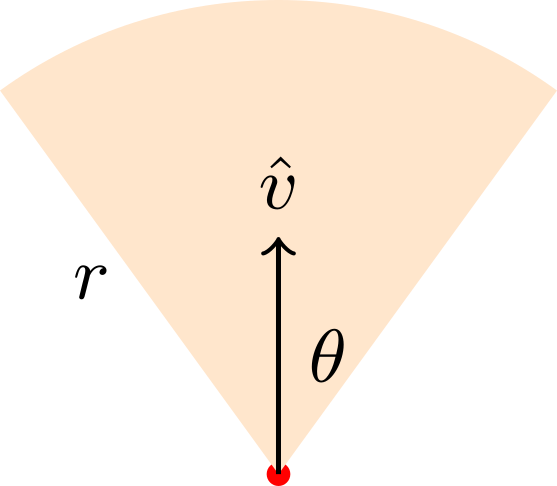
\includegraphics[width=0.3\linewidth]{immagini/fov.png}
  \caption{Rappresentazione del campo visivo di un pedone.}
  \label{fig:fov}
\end{figure}

% 2.1.3
\subsection{Movimento}
Lo spostamento dei pedoni all'interno di una folla, in maniera particolare durante un'evacuazione, non è dettato da una pianificazione del percorso da seguire ma da una serie di scelte attuate localmente analizzando le informazioni provenienti dall'ambiente circostante. Per modellare questi aspetti, mi sono avvalso dei comportamenti di steering formulati da C. W. Reynolds in \cite{Reynolds1999}, che sono alla base del movimento delle folle anche nel settore videoludico e in quello dell'animazione cinematografica. La loro funzione, infatti, è quella di muovere in maniera autonoma e realistica i personaggi su cui non si possiede il controllo, all'interno del mondo artificiale nel quale sono inseriti. \newline
Un comportamento di steering è una forza che influisce sul movimento di un agente al fine di permettergli di conseguire l'obiettivo per cui è pensato. Per determinarla ci si basa sulla semplice formula $steering = desired\_velocity - current\_velocity$, dove $current\_velocity$ è la direzione di movimento che l'agente sta seguendo, mentre $desired\_velocity$ è quella che egli vorrebbe seguire per adempiere il più velocemente possibile al suo intento. Nel caso il pedone non si stia muovendo, ovviamente, quest'ultima coinciderebbe con la forza di steering. \newline
Tra i comportamenti presenti si è focalizzata l'attenzione su quelli considerati più idonei a poter essere utilizzati nell'ambito dell'evacuazione di folle.

\paragraph{Raggiungere o fuggire}
I comportamenti più semplici a cui si può pensare nell'ambito dello steering sono il raggiungimento di un determinato punto di interesse all'interno dell'ambiente e, analogamente, la fuga da un luogo specificato, ad esempio per la presenza di un potenziale pericolo in corrispondenza ad esso.
Queste due forze, sono logicamente una l'opposto dell'altra, infatti, le $desired\_velocity$ relative ad ognuna di esse hanno direzioni contrarie.

\paragraph{Arrivare} 
Normalmente, quando un agente si trova in prossimità del punto che vuole raggiungere, esso è portato naturalmente a rallentare la propria velocità di andatura in maniera tale da arrivare a fermarsi in prossimità esatta del punto in questione. Questo risultato può essere ottenuto a partire dal già citato comportamento del raggiungimento, creando un cerchio intorno alla posizione d'interesse, detto \text{area di rallentamento} e scalando la velocità del pedone, nel caso vi si trovi all'interno di un fattore pari a $\frac{dist(p)}{radius}$, dove $dist(p)$ è la distanza corrente tra l'agente e il punto $p$ mentre $radius$ è il raggio dell'area di rallentamento.

\paragraph{Girovagare}
Volendo muovere un agente in maniera casuale si potrebbe pensare, riutilizzando concetti già analizzati, di generare periodicamente delle posizioni d'interesse fittizie all'interno dell'ambiente e di usufruire del comportamento \enquote{raggiungere} per indurre il pedone ad avvicinarvisi. Questo approccio però, potrebbe portare a movimenti innaturali dovuti a repentini cambi di direzione. \newline
Per ovviare a questo problema viene creata un circonferenza davanti dell'agente, sulla quale viene scelto casualmente un punto che sarà quello da raggiungere. Questa soluzione restringe il campo delle possibili posizioni verso cui dirigersi e determina risultati più simili al reale comportamento umano.

\paragraph{Evitare gli ostacoli} 
Considerando la potenziale presenza di ostacoli nell'ambiente, è necessario definire un comportamento di steering che permetta di schivarli in modo da evitare situazioni nelle quali un agente, a seguito di una collisione, rimanga per sempre bloccato, incapace di proseguire per via della presenza dell'ostacolo ma volendo al contempo andare al di là di esso. \newline
Ricordando che un agente ha una conoscenza limitata dell'ambiente circostante, in quanto le sue scelte sono localizzate, non viene presa in considerazione la totalità degli ostacoli presenti ma solo quello attualmente più prossimo ad esso. \newline
Per determinare il cambiamento di direzione, si usa la futura posizione di collisione e si applica una forza di repulsione considerando dove si trova il centro dell'ostacolo di riferimento. Tale formulazione, è particolarmente adatta per ostacoli di forma circolare, ma è utilizzabile potenzialmente per ogni tipo di ostacolo, approssimandone la forma a quella di un cerchio.

\paragraph{Seguire il flusso}
Il movimento di un agente potrebbe anche non essere guidato da una decisione ma da un fattore esterno in grado, direttamente o indirettamente, di determinare la prossima posizione in cui esso si troverà. Classici esempi sono le correnti d'acqua, in grado di trascinare, nel loro caotico movimento, gli eventuali oggetti che si trovano sulla loro strada, ma anche il campo magnetico, che, pur se non macroscopicamente osservabile, ha effetti evidenti in presenza di materiali ferrosi. \newline
Generalizzando questo fenomeno, è possibile modellarlo come un campo vettoriale, in cui ad ogni posizione è associata la prossima direzione da seguire che rappresenta appunto la $desired\_velocity$ di questo comportamento.

\subsubsection{Composizione di forze}
Pur potendo essere sfruttate anche singolarmente, le vere potenzialità dei comportamenti di steering possono essere apprezzate solo combinando i vari apporti tra loro in modo da ricreare dei movimenti complessi. In una situazione realistica, infatti, un pedone è in grado di decidere la prossima direzione da seguire, valutando contemporaneamente quella che gli consente di evitare gli ostacoli presenti, fuggire da situazioni di pericolo e raggiungere il prima possibile il punto di interesse. \newline
Questa tendenza è presente anche nella formulazione del modello forze sociali in tutte le sue varianti \cite{Chen2017}, dove, per ogni aspetto considerato, viene calcolata una forza che lo possa rappresentare realisticamente e tra queste viene poi eseguita la somma vettoriale per determinare la direzione e la velocità con cui il pedone deciderà di muoversi.

% 2.1.4
\subsection{Gruppi}
Considerare una folla come un aggregato di persone isolate è una semplificazione non sempre accettabile visto che più del 70\% dei pedoni si muove in gruppi \cite{Moussad2010}, che siano questi coppie, famiglie o amici. \newline
L'influenza del gruppo sul singolo individuo ad esso appartenente, è fondamentale per riprodurre dei comportamenti comuni nella vita di tutti i giorni, come la tendenza a rimanere uniti e a muoversi all'unisono aspettando coloro che sono eventualmente rimasti indietro. L'appartenenza ad un gruppo, infatti, non definisce solamente uno stato sociale per il pedone ma influisce in maniera decisiva anche sul suo movimento.

\subsubsection{Movimento collettivo}
In aggiunta ai comportamenti di steering precedentemente trattati, è possibile classificare altri atteggiamenti che scaturiscono nel pedone dalla necessità ad adattarsi al movimento degli altri individui presenti, in particolare se essi appartengono al suo stesso gruppo. \newline
Questa tendenza a conformarsi è visibile anche nel mondo naturale, dove lo spostamento in massa è una caratteristica peculiare di molte specie quali uccelli, pesci, batteri e insetti; è proprio dall'osservazione del loro comportamento che C. W. Reynolds ha formulato in \cite{Reynolds1987} le azioni alla base del movimento collettivo. \newline
Questi comportamenti, pur coinvolgendo più pedoni, sono a tutti gli effetti delle forze di steering e, in quanto tali, possono essere combinati tra loro per descrivere aspetti più complessi. Rispetto a quelli precedentemente descritti però, hanno un ruolo molto diverso. Infatti, mentre gli altri analizzano il movimento in relazione all'ambiente e non alla conformazione della folla presente, che potrebbe essere costituita anche da un solo pedone, le azioni collettive non avrebbero alcun effetto senza includere quest'ultimo aspetto. \newline
Per questo motivo, considerando l'introduzione dei gruppi nel modello forze sociali studiato in \cite{Moussad2010}, la direzione da seguire è stata calcolata considerando come contributi separati l'apporto delle semplici azioni di steering e di quelle di gruppo, piuttosto che mischiando insieme i comportamenti delle due categorie.

\paragraph{Allineamento}
La direzione e la velocità dei soggetti intorno ad un determinato pedone, determina su di esso una tendenza a conformarsi a questi parametri e a regolarli in modo da seguire il loro stesso andamento. Per riuscire in questo intento, il calcolo della direzione e del modulo della $desired\_velocity$ di questo comportamento in un pedone, viene effettuato considerando la media di questi fattori, negli individui entro una distanza massima predefinita da esso.

\paragraph{Coesione}
Analogamente a quanto definito nell'allineamento per velocità e direzione, un pedone è portato anche a spostarsi in posizioni che gli permettano di mantenere una certa vicinanza con gli altri individui presenti. Per calcolare il movimento che favorisca questo principio, si utilizza il centroide, cioè il punto medio delle posizioni attuali dei pedoni presi in considerazione. \newline
L'effetto del meccanismo di coesione tra i vari pedoni, ha ancor più rilevanza se considerato per gruppi già definiti \cite{Vizzari2013}, dove quella di rimanere uniti è la priorità anche rispetto a mettersi in salvo.

\paragraph{Separazione}
In maniera opposta al comportamento di coesione, se la densità di persone inizia a diventare proibitiva nelle immediate vicinanze di un pedone e vi è dello spazio disponibile da occupare, l'agente tenterà di andarci, in modo da ristabilire una certa distanza dagli altri e ottimizzare lo spazio che l'ambiente mette a disposizione.

\subsubsection{La presenza di leader}
Vi sono dei casi in cui i soggetti appartenenti ad un gruppo non hanno tutti la stessa rilevanza nella scelta del processo decisionale da attuare; ne è un esempio significativo quello della famiglia, in cui i figli tendono a seguire le indicazioni dei genitori, figure più consce della situazione che si è venuta a creare e con più esperienza su come risolverla. \newline
La presenza all'interno del gruppo di un leader, è un fattore determinante nello studio dell'evacuazione di folle \cite{Ji2006}\cite{Kster2011}, che agisce sensibilmente sulle scelte comportamentali degli altri membri, naturalmente portati dalla fiducia per esso, a seguire le sue indicazioni senza preoccuparsi delle eventuali conseguenze.
\section{Progettazione}

% 2.2.1
\subsection{Costruzione degli scenari}
Prima di analizzare le scelte attuate nella progettazione dei pedoni, è doveroso porre l'attenzione sugli elementi caratterizzanti lo scenario nel quale questi devono essere inseriti, in modo da capire come gli elementi appartenenti al modello di Alchemist, sono stati ampliati o adattati per essere utilizzati nel contesto dell'evacuazione di folle. 

\subsubsection{Ambienti}
Pur essendo presenti molte tipologie di ambiente in Alchemist, nessuno di questi presentava una componente fisica che si occupasse di gestire la forma geometrica dei vari nodi, al fine di impedire che questi si presentassero contemporaneamente nella stessa porzione di spazio. \newline
Questa limitazione non permetteva il verificarsi di fenomeni molto comuni, come l'accalcamento di pedoni in prossimità dell'uscita o l'intralcio nel movimento dovuto all'alta densità di persone perché, consentendo la sovrapposizione, nessun individuo poteva essere ostacolato nelle sue azioni dalla presenza degli altri. \newline
Per questo motivo, è stato introdotto il concetto di \texttt{PhysicsEnvironment}, un ambiente nel quale il movimento o il cambiamento di orientamento di un nodo è vincolato dalla non collisione con nessun altro nodo all'interno di esso. \newline
Visti gli svariati campi applicativi in cui questa soluzione si potrebbe rivelare utile, si è deciso di ristrutturare la gerarchia preesistente degli ambienti, che ora si presenta come in figura \ref{fig:environments-uml}, dove le nuove interfacce e classi inserite sono state contrassegnate con un colore leggermente più scuro.

\begin{figure}[ht]
  \centering
  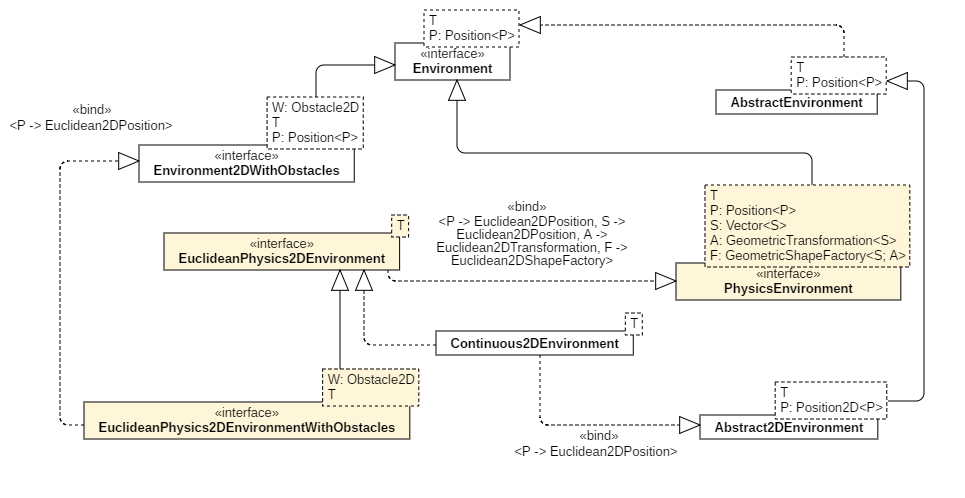
\includegraphics[width=1.0\linewidth]{immagini/uml/environments.png}
  \caption{Nuovo diagramma delle classi in UML degli ambienti in Alchemist.}
  \label{fig:environments-uml}
\end{figure}

\subsubsection{Punti di interesse}
Il solo ambiente non è sufficiente a descrivere lo scenario di interesse nel caso di un'evacuazione, infatti, è essenziale che vi sia un modo per poter rappresentare i pericoli da cui si sta scappando e i punti da raggiungere per mettersi in salvo. \newline
Per definire queste zone, è stata associata ad ognuna di esse una molecola identificativa e ci si è avvalsi dell'uso dei \texttt{Layer}, strati costitutivi la distribuzione spaziale della concentrazione di una determinata molecola all'interno dell'ambiente. \newline 
Nello specifico, sono stati utilizzati dei \texttt{BidimensionalGaussianLayer}, livelli caratterizzati da una distribuzione gaussiana delle concentrazioni, modulabili attraverso la regolazione di intensità e ampiezza per rappresentare tanto un fiammifero acceso quanto un incendio divampato. \newline
La scelta della tipologia di \texttt{Layer} è assolutamente indipendente dall'ambiente che si sta utilizzando, quindi, è possibile definire a proprio piacimento la struttura spaziale che si intende ottenere per modellare fenomeni anche meno localizzati e più irregolari rispetto a quelli sopra citati.

% 2.2.2
\subsection{Pedoni omogenei, eterogenei e cognitivi}
Partendo dal concetto di nodo in Alchemist, piuttosto che creare un unico onnicomprensivo modello di pedone, la decisione è stata di procedere analizzando tre livelli crescenti di dettaglio, nello specifico:
\begin{itemize}
    \item \textbf{Pedone omogeneo}: un nodo con una velocità predefinita di camminata e di corsa uguale per tutti.
    \item \textbf{Pedone eterogeneo}: un nodo con un sesso ed una età assegnati, dai quali saranno determinate velocità, conformità alle regole ed attitudine ad aiutare.
    \item \textbf{Pedone cognitivo}: un pedone eterogeneo con delle emozioni, capace di influenzare e farsi influenzare dagli altri.
\end{itemize}
Questo approccio rende possibile confrontare, ripetendo la stessa simulazione con tutte e tre le tipologie di pedone, il comportamento delle diverse astrazioni, in modo da valutare la rilevanza di determinate caratteristiche.
\newline
Per ogni genere di pedone, è stato definito un prototipo di base con l'obiettivo di incapsulare la gestione delle caratteristiche ad esso inerenti al suo interno. La modellazione di aspetti più strettamente collegati all'ambiente di simulazione che si sta utilizzando, come la struttura fisica, viene invece delegata a eventuali classi create estendendo tali prototipi, in modo da rendere il più agevole possibile il loro utilizzo anche in previsione di eventuali ambientazioni tridimensionali o non governate dalle leggi della geometria euclidea. \newline
Il diagramma delle classi rappresentante la struttura dei vari pedoni è presentato in figura \ref{fig:pedestrians-uml}.

\begin{figure}[ht]
  \centering
  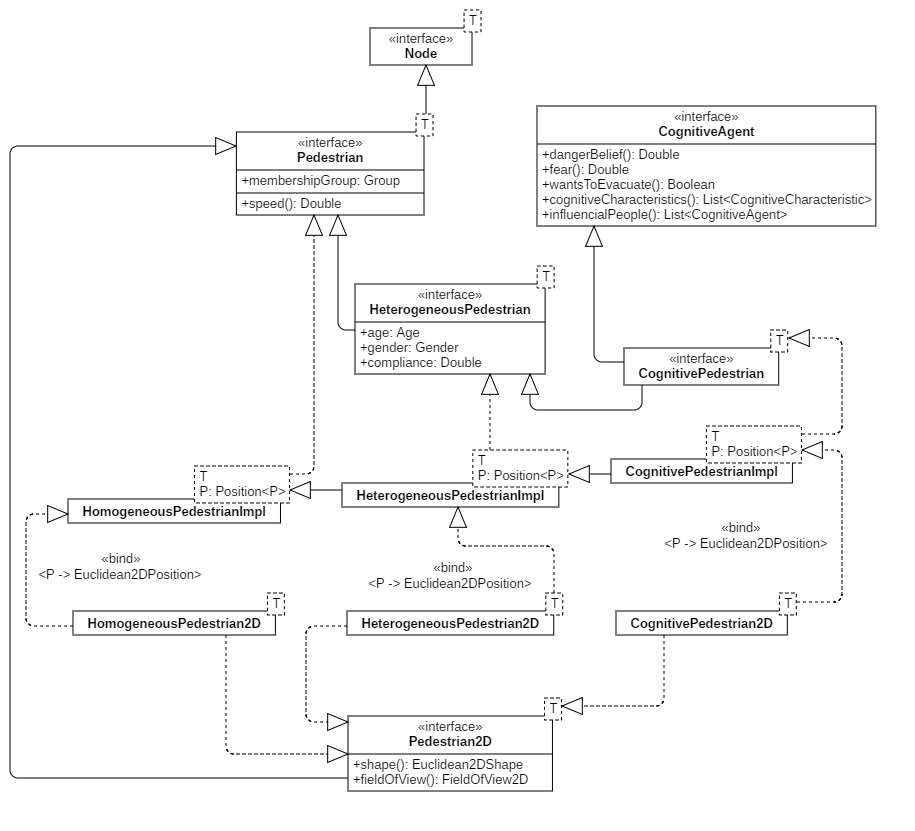
\includegraphics[width=0.8\linewidth]{immagini/uml/pedestrians.png}
  \caption{Diagramma delle classi in UML delle varie tipologie di pedone.}
  \label{fig:pedestrians-uml}
\end{figure}

\subsubsection{Pedoni bidimensionali}
Non avendo Alchemist attualmente a disposizione delle funzionalità per la simulazione tridimensionale, la concentrazione è stata focalizzata sulla creazione di pedoni bidimensionali, realizzati per ognuna delle tre categorie precedentemente descritte. \newline
Questi pedoni, la cui forma è stata approssimata a quella di un cerchio, hanno sia il vincolo di dover essere inseriti in un \texttt{EuclideanPhysics2DEnvironment}, un ambiente caratterizzato da una componente fisica e governato dalle leggi della geometria euclidea, sia la restrizione di poter essere equipaggiati solamente con delle sfere di influenza bidimensionali, come il \texttt{FieldOfView2D}. \newline
Nonostante questa scelta possa sembrare limitativa, garantisce la consistenza tra i vari elementi all'interno della simulazione ed esplicita immediatamente gli scenari in cui è idoneo utilizzare questa tipologia di nodo.

% 2.2.3
\subsection{Fenomeni cognitivi}
Per una migliore organizzazione, si è deciso di suddividere le caratteristiche inerenti i pedoni in due categorie a seconda della loro funzione:
\begin{itemize}
    \item \textbf{Caratteristiche individuali}: intrinsecamente parte del pedone e non mutabili nel corso della simulazione. Appartengono a questa categoria: età, sesso, velocità, conformità alle regole, ed attitudine ad aiutare.
    \item \textbf{Caratteristiche cognitive}: costitutive della componente relazionale ed emotiva del pedone e variabili nel corso della simulazione. Appartengono a questa categoria: sensazione di pericolo, paura, desiderio di fuggire e di non fuggire, intenzione di fuggire e di non fuggire.
\end{itemize}
Tale suddivisione ha permesso di sfruttare, nel caso delle caratteristiche cognitive, i vantaggi del pattern comportamentale \textit{template method} \cite{GoF1995}, illustrato in figura \ref{fig:cognitive-characteristics-uml}, con il quale sono state ristrutturate le equazioni differenziali relative ad ogni caratteristica. Ad ognuna di esse è stata associata solamente la relativa funzione di combinazione $c_{y}$ ed è stato così ridotto il rischio di errore in fase di implementazione, ma anche il grado di difficoltà di comprensione in caso di futura modifica. \newline
Per quanto riguarda la gestione dell'evoluzione dei processi emotivi, è stata creata una reazione responsabile di questo tipo di comportamenti, incaricata di risolvere per ogni emozione considerata, l'equazione ad essa relativa. \newline
Le caratteristiche inerenti i pedoni sono state modellate in maniera completamente indipendenti dalla struttura di Alchemist, con l'obiettivo di poterle estrapolare e riutilizzare anche in altri contesti applicativi.

\begin{figure}[ht]
  \centering
  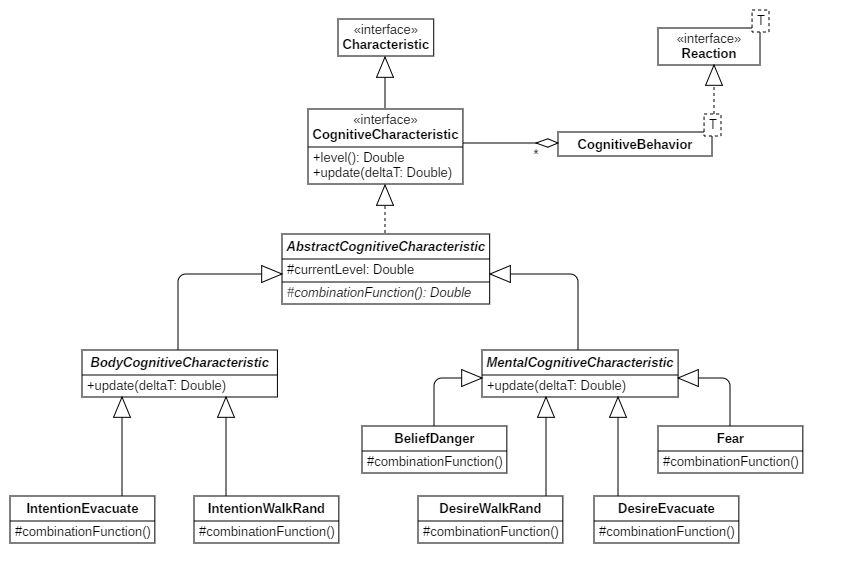
\includegraphics[width=0.8\linewidth]{immagini/uml/cognitive-characteristics.png}
  \caption{Diagramma delle classi in UML delle caratteristiche cognitive di un agente.}
  \label{fig:cognitive-characteristics-uml}
\end{figure}

% 2.2.4
\subsection{Comportamenti di steering}
É stata utilizzata come punto di partenza l'azione \texttt{AbstractConfigurableMoveNode}, che permette di scegliere il punto di arrivo, la rotta da seguire e la velocità alla quale procedere. Si è arrivati così a definire un'implementazione comune ai vari comportamenti di steering. \newline
Al fine di non vincolare al mondo euclideo questi aspetti, che potrebbero essere utilizzati anche in ambiti dove tale geometria non è valida, si è deciso di mantenere generica la tipologia di posizione utilizzata. Un esempio è quello del traffico stradale, dove ad una vettura non è sempre concesso proseguire in entrambi i sensi di marcia. \newline
Per rappresentare il flusso da seguire, si è fatto uso di \texttt{Layer} e sono state emulate le direzioni costituenti il campo vettoriale sfruttando la differenza di concentrazione della molecola ad esso associata, tra due diversi punti dello spazio. Grazie a questa scelta, il pedone può essere alternativamente mosso verso posizioni contraddistinte da un gradiente sempre maggiore o da uno sempre minore. \newline
Oltre alle azioni di steering formulate da Reynolds, ne è stata introdotta una denominata \texttt{Combine}, responsabile di determinare la rotta finale da far seguire al pedone combinando quelle di tutte le altre presenti.

\begin{figure}[ht]
  \centering
  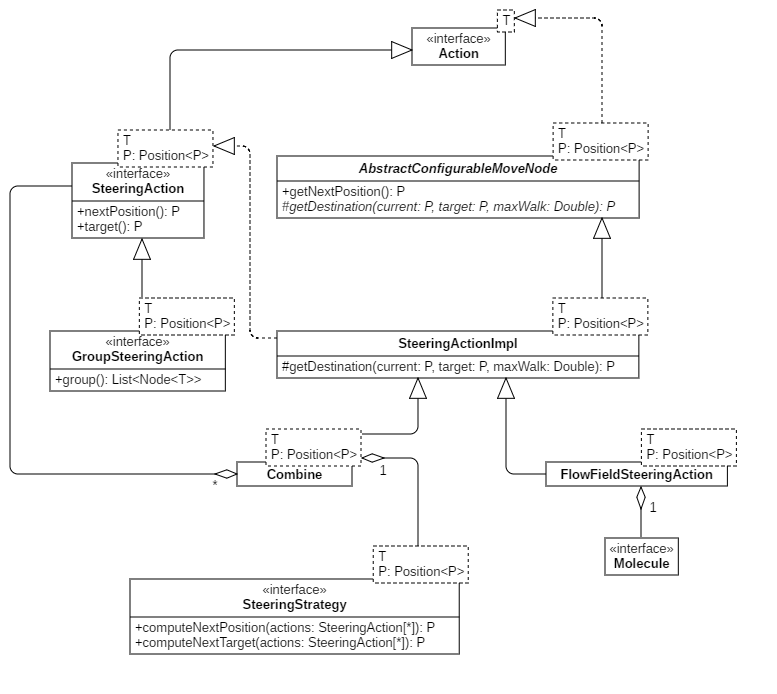
\includegraphics[width=0.8\linewidth]{immagini/uml/steering-actions.png}
  \caption{Diagramma delle classi in UML della struttura delle azioni di steering.}
  \label{fig:steering-actions-uml}
\end{figure}

% 2.2.5
\subsection{Strategie di steering}
Il movimento dei pedoni, pur differenziandosi in relazione alle caratteristiche associate ad ognuno di essi, consiste sempre nella combinazione di multiple azioni di steering, che determinano la direzione da seguire al fine di conseguire tutti gli obiettivi prefissati. \newline
Cercando di realizzare questo principio, attraverso la somma vettoriale delle varie forze di steering tuttavia, è possibile incorrere in problemi di stallo o movimenti impredicibili, dovuti all'inibizione o addirittura all'annullamento di forze che, per motivi strutturali, sono una l'opposto dell'altra. \newline
Per differenziare l'attitudine del pedone a compiere una determinata azione piuttosto che un'altra sono state formulate delle strategie, algoritmi attraverso i quali modificare il modulo delle forze valutate per aumentarne o diminuirne l'influenza nel calcolo della direzione finale. \newline 
Il modulo della forza risultante è irrilevante ai fini della rapidità di spostamento del pedone, che è invece determinata dalla sua velocità. \newline 
Non essendovi delle regole ben precise per calcolare la rilevanza di ogni forza rispetto alle altre e dipendendo tale calcolo anche dallo scenario preso in considerazione, si è mantenuta la modellazione il più generale possibile. \newline 
In particolare sono state formulate alcune strategie di esempio, in modo da fornire una base di partenza per la creazione di eventuali altre:

\begin{itemize}
    \item \textbf{Basata sul peso}: Ad ogni azione viene associato un peso con una funzione di mapping e viene poi eseguita la somma vettoriale pesata. 

    \item \textbf{Basata sulla distanza}: Utilizza come metrica per determinare il peso di una azione di steering, la distanza tra il punto designato come da raggiungere in essa e la posizione attuale del pedone.

    \item \textbf{Massima vicinanza}: Valuta solo l'azione di steering che, considerata la posizione attuale del pedone, è quella con il punto da raggiungere più vicino ad essa.

    \item \textbf{Basata sul tipo}: Utilizza come metrica per determinare il peso, un valore associato ad ogni tipologia di azione di steering, grazie al quale, ad esempio, è possibile enfatizzare l'importanza della fuga dal pericolo, piuttosto che quella del movimento casuale.
\end{itemize}

Per massimizzare il riutilizzo delle varie logiche di steering, si è fatto uso del pattern strutturale \textit{decorator} \cite{GoF1995} creando una strategia \texttt{Filtered} con l'obiettivo di utilizzare una stessa logica su un più ristretto numero di azioni. Lo schema relativo alla struttura adottata è mostrato in figura \ref{fig:steering-strategies-uml}. \newline
Per eseguire le azioni di steering in combinazione tra loro e non una di seguito all'altra, ha avuto un ruolo decisivo la realizzazione della reazione \texttt{SteeringBehavior}, capace di riconoscere ed eseguire congiuntamente solo questo tipo di azioni tra tutte le varie presenti. Per permettere di scegliere al momento della scrittura della simulazione la strategia di steering da utilizzare, è stato sfruttato il pattern comportamentale \textit{strategy} per definire versioni più specifiche di questa reazione. \newline 
In particolare, a fine esemplificativo, sono stati differenziati un \texttt{PrioritySteering}, per indicare l'uso della strategia di massima vicinanza ed un \texttt{BlendedSteering}, per indicare l'uso della logica basata sulla distanza.

\begin{figure}
  \centering
  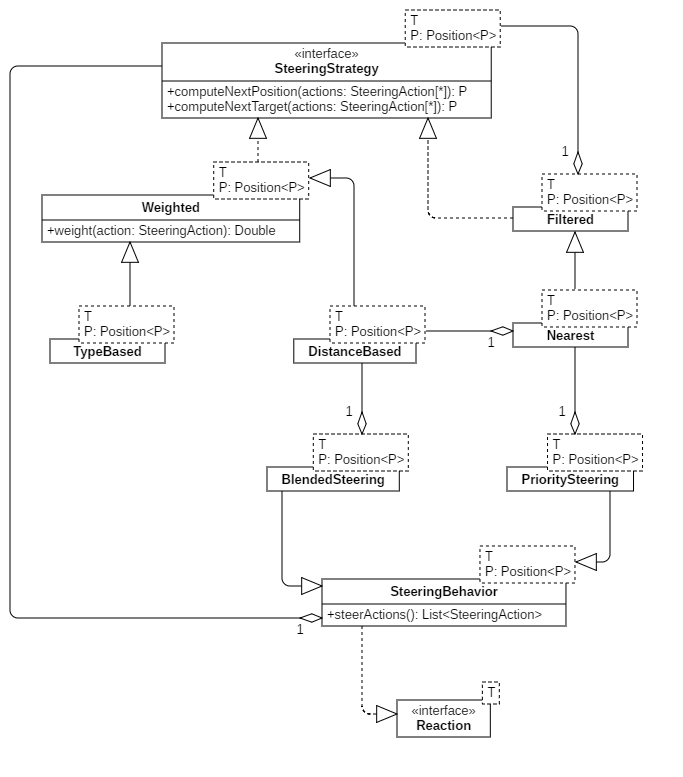
\includegraphics[width=0.75\linewidth]{immagini/uml/steering-strategies.png}
  \caption{Diagramma delle classi in UML delle strategie di steering e dei relativi comportamenti.}
  \label{fig:steering-strategies-uml}
\end{figure}

% 2.2.6
\subsection{Appartenenza ad un gruppo}
Non essendo presente un concetto analogo a quello di gruppo in Alchemist, si è deciso di introdurlo generalizzandolo per qualsiasi tipologia di nodo, in modo da poterlo impiegare anche in contesti non esplicitamente inerenti i pedoni, quali quelli del mondo animale. \newline
Per favorire l'assegnamento del gruppo di appartenenza durante il caricamento della simulazione, nello specifico durante la creazione dei nodi, viene lasciata la possibilità di aggiungere o rimuovere dei membri al suo interno. \newline
Nei gruppi in cui un elemento assume il ruolo di leader, per decidere quale membro in particolare sia degno di questo incarico, si è utilizzato un comparatore, grazie al quale è possibile usare la logica che più si ritiene opportuna per selezionare un nodo piuttosto che un altro. \newline 
Essendo questo lavoro incentrato sulle persone, le tipologie di gruppo presentate come esempio sono: \texttt{Alone} per indicare il caso limite di un pedone solitario, \texttt{Friends} per un generico insieme in cui ogni membro ha le stesse responsabilità degli altri e \texttt{Family} in modo da fornire anche un riscontro pratico alla presenza di leader. \newline
La struttura risultante è schematizzata in figura \ref{fig:groups-uml}.

\begin{figure}[ht]
  \centering
  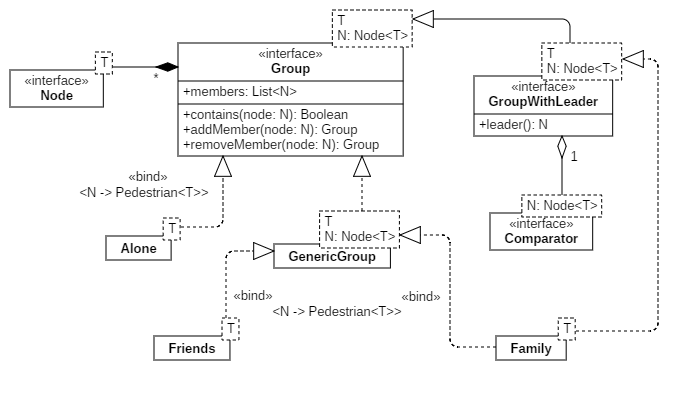
\includegraphics[width=0.75\linewidth]{immagini/uml/groups.png}
  \caption{Diagramma delle classi in UML dei gruppi.}
  \label{fig:groups-uml}
\end{figure}
\section{Implementazione}

% 2.3.1
\subsection{Metodologia di lavoro}
Alchemist è sviluppato facendo uso delle pratiche tipiche della metodologia DevOps\n{\url{https://aws.amazon.com/it/devops/what-is-devops/}}, particolarmente adatta nel caso di un software di medio-grandi dimensioni con rilasci frequenti.

\subsubsection{Divisione in moduli}
L'implementazione degli agenti cognitivi e del loro ecosistema all'interno di Alchemist, è stata strutturata in maniera trasversale rispetto all'incarnazione che si sarebbe poi utilizzata per effettuare le simulazioni. Questa proprietà, rende le classi introdotte flessibili a poter essere utilizzate oltre che in quelle già esistenti, anche in possibili future incarnazioni maggiormente incentrate sul comportamento delle folle. \newline
Al fine di aderire alla struttura attuale di Alchemist incentrata sulla modularità, sono stati creati i moduli \texttt{alchemist-influence-sphere}, per la realizzazione delle sfere di influenza e \texttt{alchemist-cognitive-agents}, per l'implementazione dei pedoni e delle azioni, reazioni e caratteristiche ad essi relative. \newline
Tale struttura ha portato notevoli benefici in fase di sviluppo, garantendo la possibilità di mantenere separato e circoscritto il proprio spazio di lavoro rispetto al resto del simulatore e quindi facilitando anche le fasi di refactoring e testing del codice.

\subsubsection{Divisione in package}
Internamente ad ogni modulo, tutte le entità derivanti dal modello alla base di Alchemist sono state organizzate mantenendo la struttura dei package originale, che prevede una netta separazione tra interfacce e relative implementazioni. Per differenziare le nuove tipologie di nodo, azione, reazione o condizione, è stato definito un package per ognuno di questi elementi. \newline
Utilizzare questi accorgimenti, permette durante la scrittura delle simulazioni in linguaggio YAML, di specificare il tipo di un oggetto direttamente utilizzando il nome della classe, mentre altrimenti sarebbe stato necessario anche l'intero package di appartenenza. \newline
Per quanto riguarda le caratteristiche dei pedoni, costruite in maniera indipendente rispetto all'architettura del simulatore, è stata invece adottata una suddivisione tematica, differenziando le caratteristiche individuali da quelle cognitive al fine di mantenere separate queste due categorie, in previsione dell'arricchimento con nuove proprietà appartenenti all'una o all'altra.

\subsubsection{Strumenti di sviluppo}

\paragraph{Git}
Git\n{\url{https://git-scm.com}} è un sistema per il controllo di versione distribuito (DVCS), che permette di gestire e supervisionare lo sviluppo del software che si sta costruendo, mantenendo ed organizzando uno storico delle modifiche effettuate. Una delle sue funzionalità, è quella di consentire di mantenere più versioni dello stesso sistema, tipicamente una stabile ed una in fase sperimentale, grazie alle quali si è in grado di fronteggiare facilmente i vari casi di malfunzionamento che si potrebbero incontrare durante l'implementazione. \newline
Alchemist utilizza la metodologia Gitflow\n{\url{https://nvie.com/posts/a-successful-git-branching-model/}} per la gestione dei vari rami di sviluppo e obbliga ogni contributore a creare una propria \textit{fork} del progetto principale, a lavorare su di essa e a contribuire con il meccanismo delle \textit{pull requests}, per integrare all'interno della versione originale del simulatore le modifiche apportate.

\paragraph{Gradle}
Gradle\n{\url{https://gradle.org}} è uno strumento per l'automazione della costruzione del software, organizzato in task per semplificare la compilazione del codice sorgente, la risoluzione delle dipendenze, l'esecuzione dei test automatici e il controllo di qualità del codice. I comandi che si intendono lanciare possono essere liberamente personalizzati dallo sviluppatore, che può creare degli script utilizzando alternativamente il DSL\n{linguaggio specifico di dominio} Groovy o una sua variante basata su Kotlin. \newline
Il simulatore Alchemist, mantiene, oltre a quello generale di progetto, uno script Gradle per ogni modulo presente al suo interno, nel quale sono specificati tutti e soli gli altri moduli o eventuali librerie esterne di cui si vogliono utilizzare le funzionalità.

\paragraph{Travis CI}
Travis\n{\url{https://travis-ci.org}} è un servizio di integrazione continua che, garantendo piena compatibilità con la piattaforma di hosting per progetti GitHub, offre la possibilità di monitorare il comportamento del sistema software allo stato attuale, installandolo ed eseguendolo su diverse macchine virtuali, con diversi sistemi operativi e diverse configurazioni. \newline
Questa possibilità, permette di tenere sempre sotto controllo la retrocompatibilità ed il supporto multi-piattaforma del simulatore, testandone il funzionamento con diverse versioni della JVM su tutti i principali sistemi operativi.

\paragraph{Orchid}
La scrittura e la manutenzione della documentazione relativa alle classi e alle interfacce presenti nel simulatore è una fase essenziale del processo di sviluppo, in quanto è solo facendo riferimento ad essa che è plausibile orientarsi all'interno di un progetto vasto come Alchemist. \newline
Orchid\n{\url{https://orchid.netlify.com}} mette a disposizione un motore per la generazione di pagine web statiche completamente integrato nel progetto, cioè utilizzabile anche mediante Gradle, con il quale è possibile ottenere un sito comprensivo di documentazione estrapolata dal codice sorgente, automaticamente aggiornato ad ogni cambiamento di API.

% 2.3.2
\subsection{Il linguaggio Kotlin}
Kotlin\n{\url{https://kotlinlang.org}} è un linguaggio di programmazione nato nel 2011 come progetto open source dell'azienda JetBrains, specializzata nello sviluppo software. \newline
La sua principale caratteristica è quella di essere pienamente interoperabile con il linguaggio Java e la Java Virtual Machine (JVM) e cioè di poter sfruttare tutta l'immensa disponibilità di librerie presenti per essi e al contempo di poter essere importato all'interno di codice Java senza riscontrare particolari problemi. \newline
Kotlin è un linguaggio multi-paradigma, in quanto presenta sia caratteristiche tipiche della programmazione orientata agli oggetti sia del paradigma funzionale, e multi-piattaforma, poiché, oltre che per la JVM, può essere compilato per Android, iOS, JavaScript e nativamente per Windows, Linux e MacOS; anche se quest'ultima funzionalità è ancora in fase sperimentale. \newline
Pur riuscendo un programmatore Java ad iniziare a sviluppare in Kotlin abbastanza agilmente, per uno studio più approfondito del linguaggio e dei suoi vari aspetti più avanzati si consiglia la lettura del libro \enquote{Kotlin in Action} \cite{Jemerov2017}.

\subsubsection{Benefici riscontrati}
La scelta dell'uso di Kotlin piuttosto che Java per l'implementazione degli agenti cognitivi all'interno di Alchemist, si è rilevata molto vantaggiosa in diversi frangenti, nei quali altrimenti, per ottenere lo stesso risultato, si sarebbe dovuto adottare soluzioni molto più verbose e di difficile comprensione.

\paragraph{Conciso} Per facilitare la fase di scrittura della simulazione all'interno del file YAML, si è voluto lasciare massima libertà all'utente sulla tipologia e sulla quantità di parametri da inserire per costruire un pedone. Tra i compromessi adottati, é permesso specificare con una stringa significativa invece che instanziare una variabile di tipo \texttt{Age} o \texttt{Gender}, per codificare l'età e il sesso del pedone da caricare.  \newline
Al fine di ottenere questo risultato utilizzando Java, sarebbe stato obbligatorio utilizzare molteplici costruttori ognuno con un differente tipo di variabile o con un numero diverso di parametri; grazie all'uso dell'annotazione \texttt{@JvmOverloads}, invece, l'incombenza di generare questo codice boilerplate viene affidata al compilatore.

\paragraph{Gestione dei null} Per cercare di prevenire la nascita di \texttt{NullPointerException}, Kotlin cerca di forzare il programmatore a non utilizzare delle variabili il cui tipo permetta che esse assumano il valore \texttt{null}. \newline 
Per aderire a questa scelta, il gruppo di appartenenza è stato pensato come una proprietà non annullabile e non modificabile del pedone, che in quanto tale, deve sempre esistere, anche nel caso in cui esso sia l'unico elemento a costituirlo. \newline
Durante la scrittura di una simulazione, tuttavia, per assegnare un gruppo ad un pedone è necessario istanziarlo all'interno della sezione \texttt{variables} e poi utilizzare il riferimento a tale variabile come parametro.
Nel caso in cui il pedone non sia parte di un gruppo ma indipendente, questa procedura richiede molta verbosità, infatti sarebbe necessario creare un gruppo di tipo \texttt{Alone} per ogni pedone solitario presente e non si potrebbe trarre vantaggio dal caricamento multiplo di nodi supportato dal simulatore. \newline
Per risolvere questo problema, si è permesso all'utente di specificare opzionalmente il gruppo di appartenenza del pedone nel file YAML ma tramite l'operatore delegato \texttt{lazy}, questo viene inizializzato in un secondo momento al gruppo inserito o, se non specificato, ad una nuova istanza di \texttt{Alone}.

\paragraph{Funzioni di estensione} Capita spesso di voler utilizzare una funzionalità per cui una classe sarebbe predisposta ma che non è stata inclusa tra i metodi pubblici ad essa appartenenti. Le funzioni di estensione propongono un'elegante soluzione a questo problema senza modificare le API della classe in questione o fare uso di metodi statici, meno espressivi dell'intento della funzione. \newline 
Dovendo implementare delle azioni inerenti il movimento di pedoni, si è avuta questa necessità per effettuare delle trasformazioni sulle posizioni, come la moltiplicazione di ogni coordinata per una stessa costante o la rotazione considerando un determinato angolo. Tali funzionalità, seppur molto comode da avere a disposizione nell'interfaccia \texttt{Position}, avrebbero potuto fuorviare l'utente sul reale intento dell'astrazione in questione, il cui ruolo è quello di modellare il concetto di posizione all'interno dell'ambiente, non di operare su di esso. \newline
Ancora più significativo, è il caso dell'interfaccia \texttt{RandomGenerator}, che, appartenendo alla libreria Apache Commons, non poteva essere modificata e quindi ampliata con ulteriori metodi quali ad esempio la generazione di numeri in virgola mobile compresi tra due estremi arbitrari.

% 2.3.3
\subsection{Librerie esterne}

\paragraph{Konf}
Essendo presenti molti parametri personalizzabili, soprattutto relativamente ai pesi riportati in tabella \ref{table:weights-impact}, si è ritenuto necessario impostare tali valori in un file esterno di configurazione salvato in formato TOML\n{\url{https://github.com/toml-lang/toml}}, standard di serializzazione considerato tra i più leggibili per un essere umano. \newline
Per riuscire ad importare all'interno delle classi di interesse i parametri contenuti in questo file, si è fatto uso della libreria Konf\n{\url{https://github.com/uchuhimo/konf}}, la quale offre il supporto e l'intercompatibilità tra tutti i principali formati di configurazione.
Per un corretto utilizzo è necessario riportare i nomi dei parametri che si vogliono leggere in una classe di specificazione creata estendendo \texttt{ConfigSpec} e fornire il percorso relativo alla risorsa in questione.

% 2.3.4
\subsection{Testing}
Parallelamente alla fase di sviluppo è stata portata avanti un'attività di \textit{unit testing} per ogni nuova funzionalità introdotta, con lo scopo di verificarne il corretto funzionamento immediato ma soprattutto quello futuro, impedendo che nuove modifiche introdotte nel simulatore possano compromettere il suo stato di avanzamento attuale. \newline
Per facilitare la creazione dei test, è stata scelta la libreria KotlinTest\n{\url{https://github.com/kotlintest/kotlintest}}, grazie alla quale è stato possibile esprimere in linguaggio naturale non solo la descrizione inerente gli aspetti da collaudare ma anche i metodi predisposti al confronto per la valutazione della correttezza del test eseguito. \newline
Quasi sempre, al fine di creare dei test significativi, è stato necessario ideare una simulazione specifica per essa, caricarla da un file YAML, eseguirla considerando un numero idoneo di passi temporali ed infine determinarne il buon esito o il fallimento, confrontando la situazione iniziale e quella finale, valutando eventualmente anche gli stadi intermedi.
\page{empty}

\chapter{Casi di studio}
Per evidenziare le potenzialità degli agenti cognitivi introdotti in Alchemist sono stati definiti alcuni casi di studio, ognuno inerente un particolare aspetto: l'influenza dell'appartenenza ad un gruppo per il singolo pedone, il contagio sociale che determina la trasmissione delle emozioni tra i vari agenti, la scelta della strategia di evacuazione da attuare in caso di ambientazioni caratterizzate da molteplici punti di interesse, la gestione del movimento in presenza di ostacoli nell'ambiente. \newline
Per ogni caso presentato, vengono confrontati i risultati della medesima simulazione eseguita prima omettendo la proprietà che si vuole sottolineare, poi considerandola; in modo da capire quale sia stato il reale apporto scaturito dalla sua introduzione. 

\section{Influenza del gruppo}
In presenza di un pericolo abbiamo tutti una naturale propensione a scappare. Questo atteggiamento, però, può subire delle variazioni se ad interessarci non è solo la nostra incolumità, ma anche quella di coloro tra i presenti con i quali abbiamo una particolare relazione affettiva. \newline
\enquote{Una famiglia sopravvive insieme o muore insieme} \cite{Kster2011} è un'affermazione che in maniera molto esplicita, sottolinea la validità di questo principio e nella quale probabilmente, tutti ci sentiamo immedesimati.

\subsection{Descrizione della simulazione}
In un ambiente euclideo continuo ed illimitato è stata inserita una fonte di pericolo al centro ed intorno ad essa sono stati disposti in maniera casuale 24 persone. \newline
Si sono effettuate due simulazioni: nella prima non considerando l'esistenza di eventuali gruppi costituiti da più agenti, mentre nella seconda specificando quattro diversi insiemi di amici di dimensioni variabili. In quest'ultimo caso, ogni agente è stato assegnato ad un gruppo senza tenere in considerazione la posizione reciproca, quindi ammettendo anche il caso di membri molto lontani tra loro nell'ambiente. \newline
Per indurre il movimento, si è scelta la reazione \texttt{BlendedSteering}, con la quale vengono uniti il meccanismo di coesione ed il comportamento di steering dell'inseguimento del flusso, rappresentante un allontanamento dalla fonte di pericolo.

\subsection{Risultati ottenuti}
Confrontando i fotogrammi della simulazione con solo pedoni solitari (figura \ref{fig:influence-without-groups}) rispetto a quelli della simulazione con gruppi di dimensioni maggiori (figura \ref{fig:influence-with-groups}), il comportamento che si riscontra è indubbiamente differente. \newline
Come era prevedibile, quando un pedone non è vincolato dalla presenza di altri membri nel suo gruppo, cerca solamente di allontanarsi il più possibile dal pericolo. \newline 
Al contrario, se è condizionato dalla necessità di ricongiungersi con qualcun altro, lo si vede muovere intorno alla zona di rischio alla sua ricerca. Solo una volta che tutto il gruppo si è ricongiunto, i vari membri che lo compongono procedono ad allontanarsi il più possibile.

\begin{figure}
    \centering
    \begin{subfigure}[b]{0.75\textwidth}
        \centering
        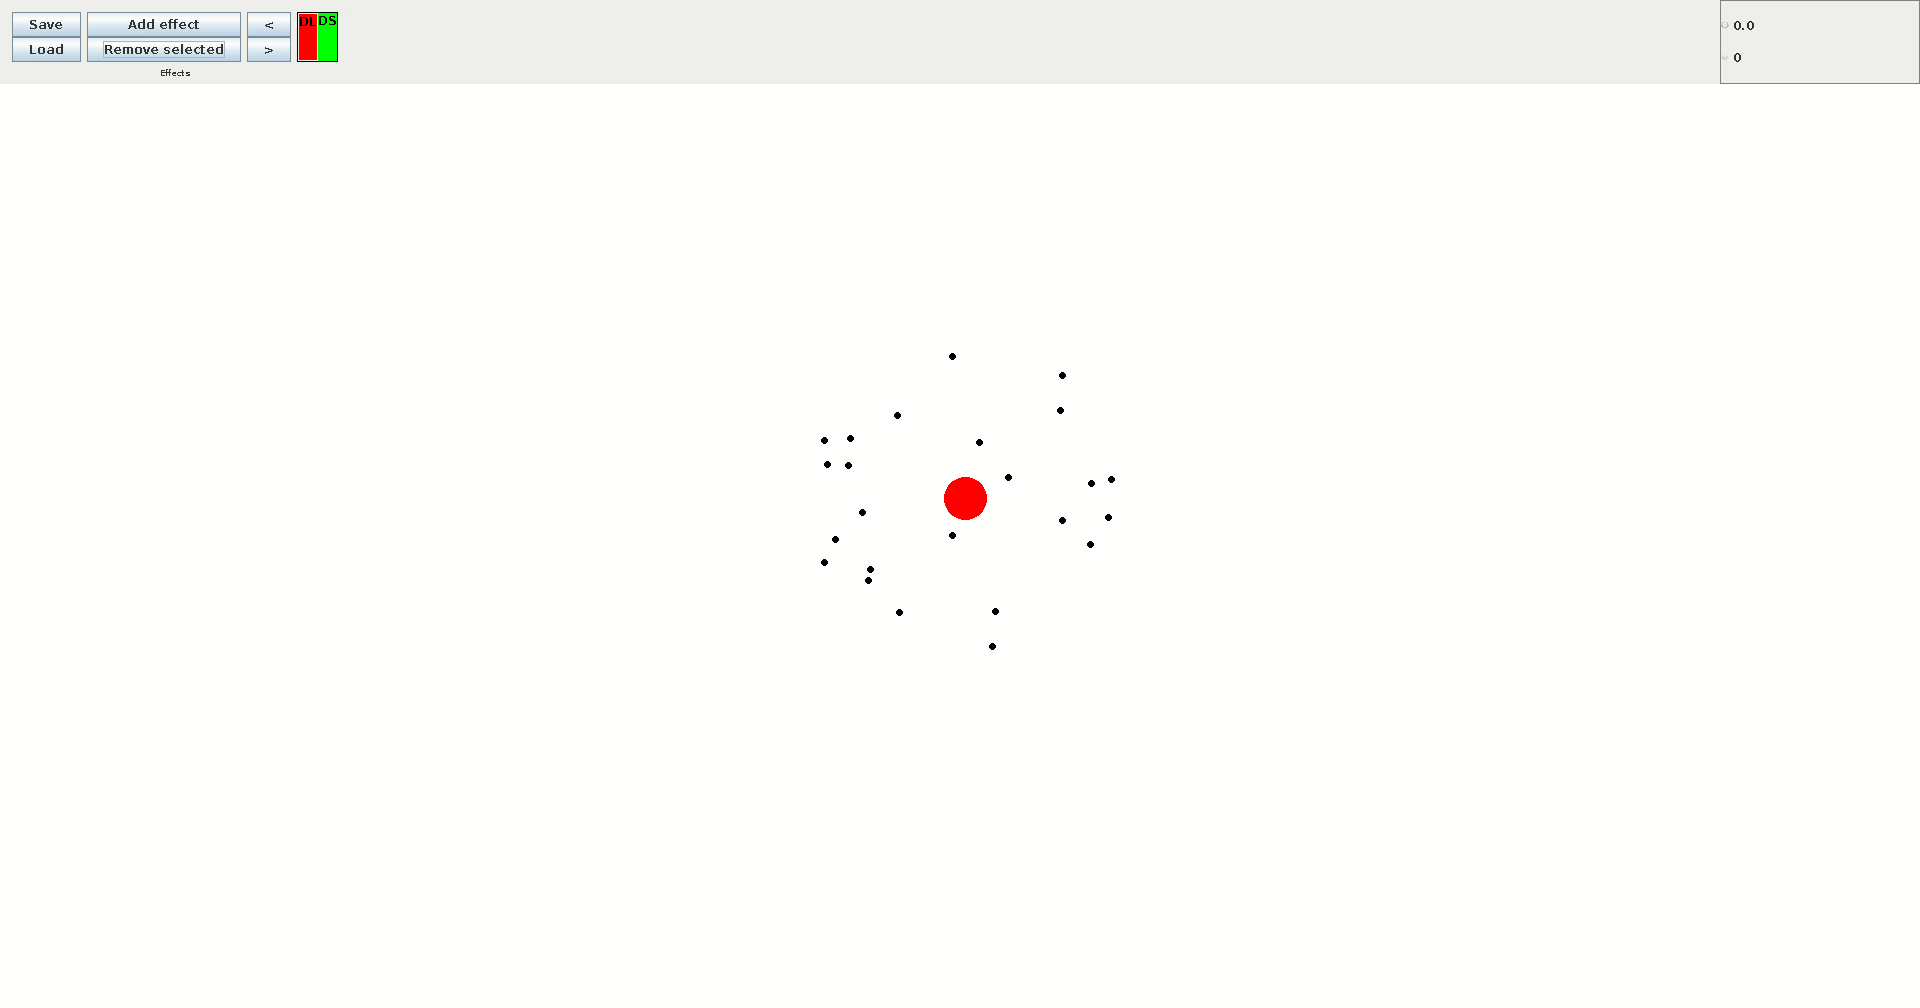
\includegraphics[width=\textwidth]{immagini/casi-studio/influence-without-groups-begin.png}
    \end{subfigure}
    \hfill
    \begin{subfigure}[b]{0.75\textwidth}
        \centering
        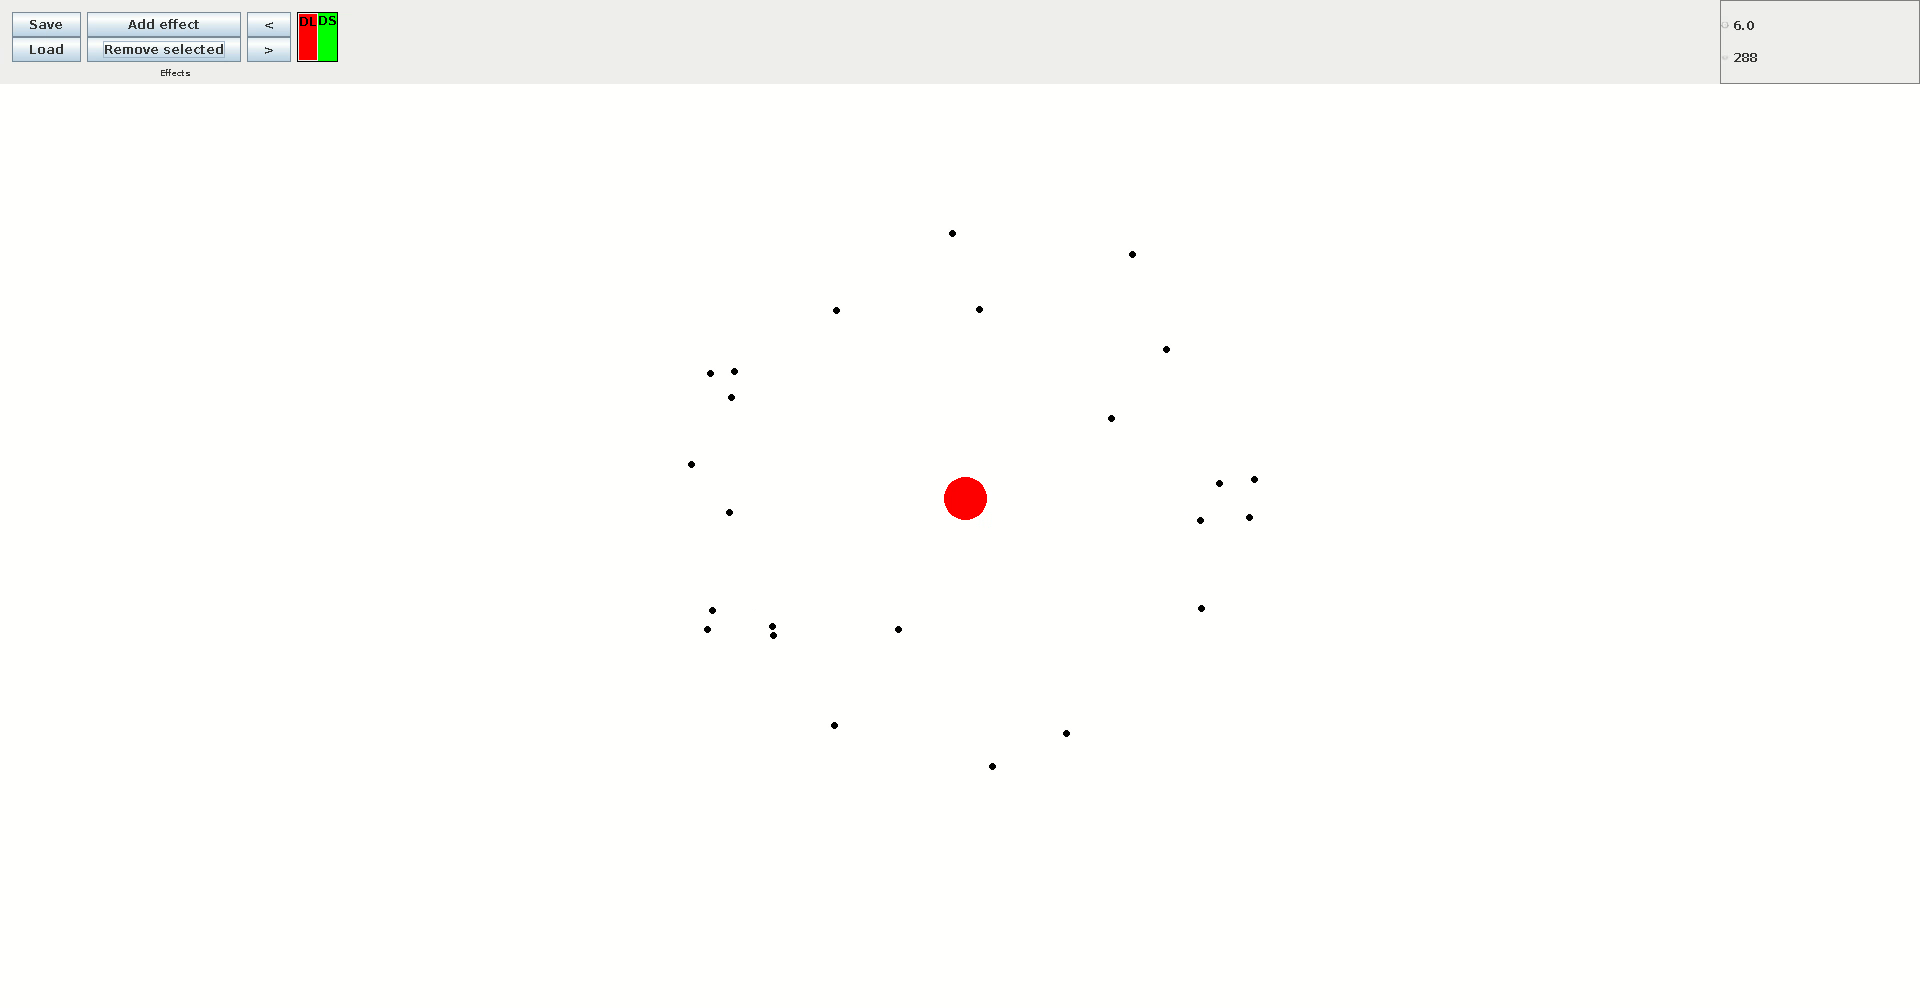
\includegraphics[width=\textwidth]{immagini/casi-studio/influence-without-groups-during.png}
    \end{subfigure}
    \hfill
    \begin{subfigure}[b]{0.75\textwidth}
        \centering
        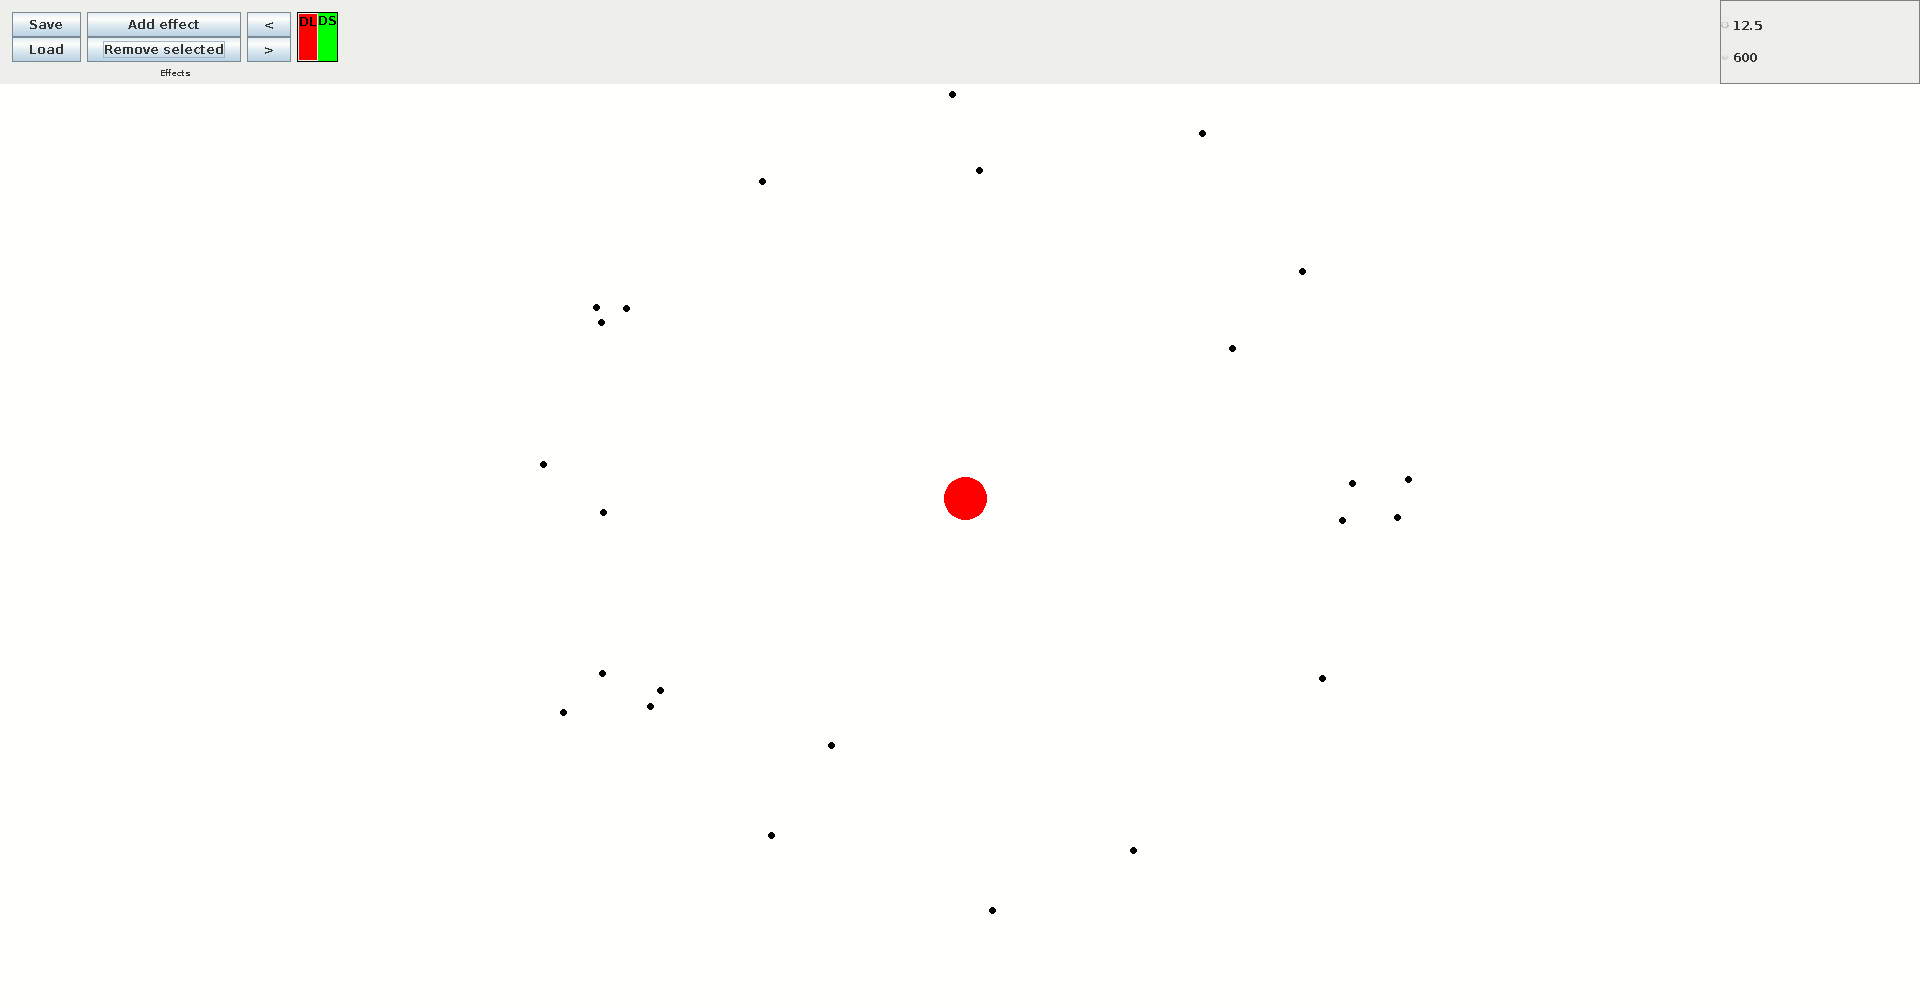
\includegraphics[width=\textwidth]{immagini/casi-studio/influence-without-groups-end.png}
    \end{subfigure}
    \caption{Fotogrammi salienti della simulazione sull'influenza del gruppo considerando pedoni solitari; è possibile notare come essi, pensando solo alla propria incolumità, si limitino a fuggire dalla zona di pericolo.}
    \label{fig:influence-without-groups}
\end{figure}

\begin{figure}
    \centering
    \begin{subfigure}[b]{0.75\textwidth}
        \centering
        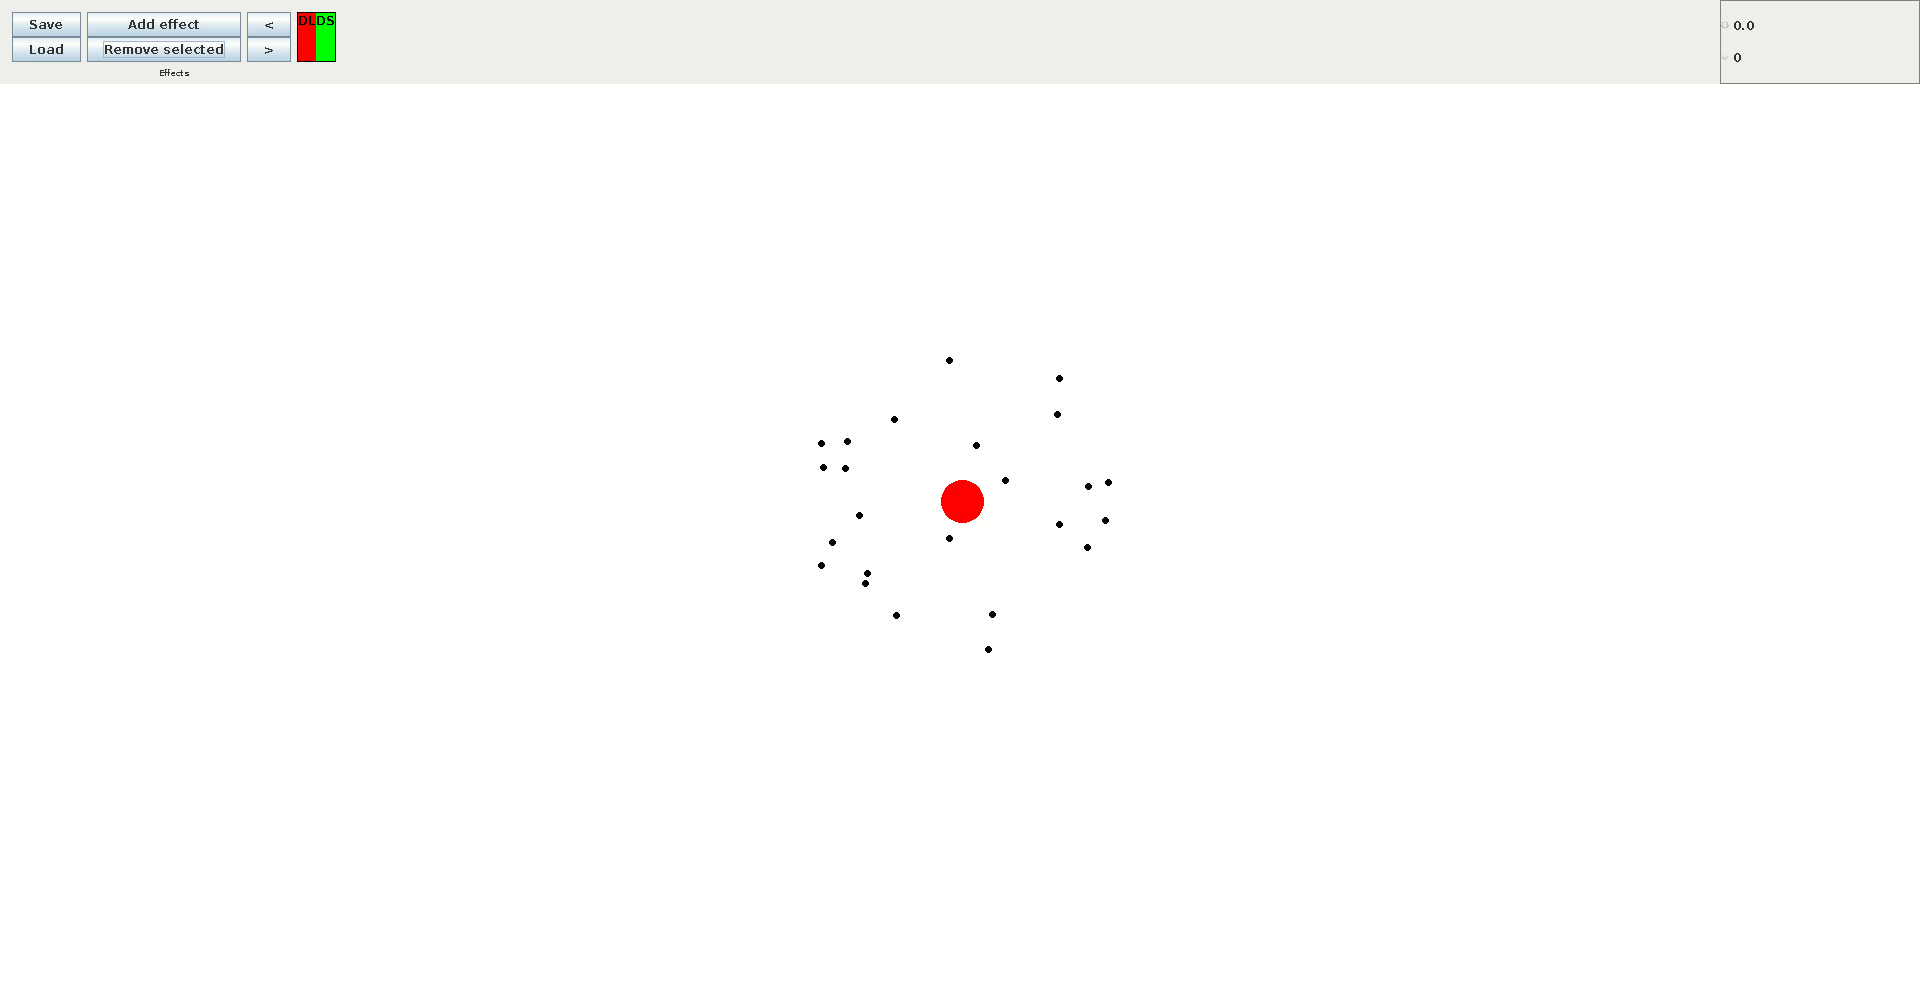
\includegraphics[width=\textwidth]{immagini/casi-studio/influence-with-groups-begin.png}
    \end{subfigure}
    \hfill
    \begin{subfigure}[b]{0.75\textwidth}
        \centering
        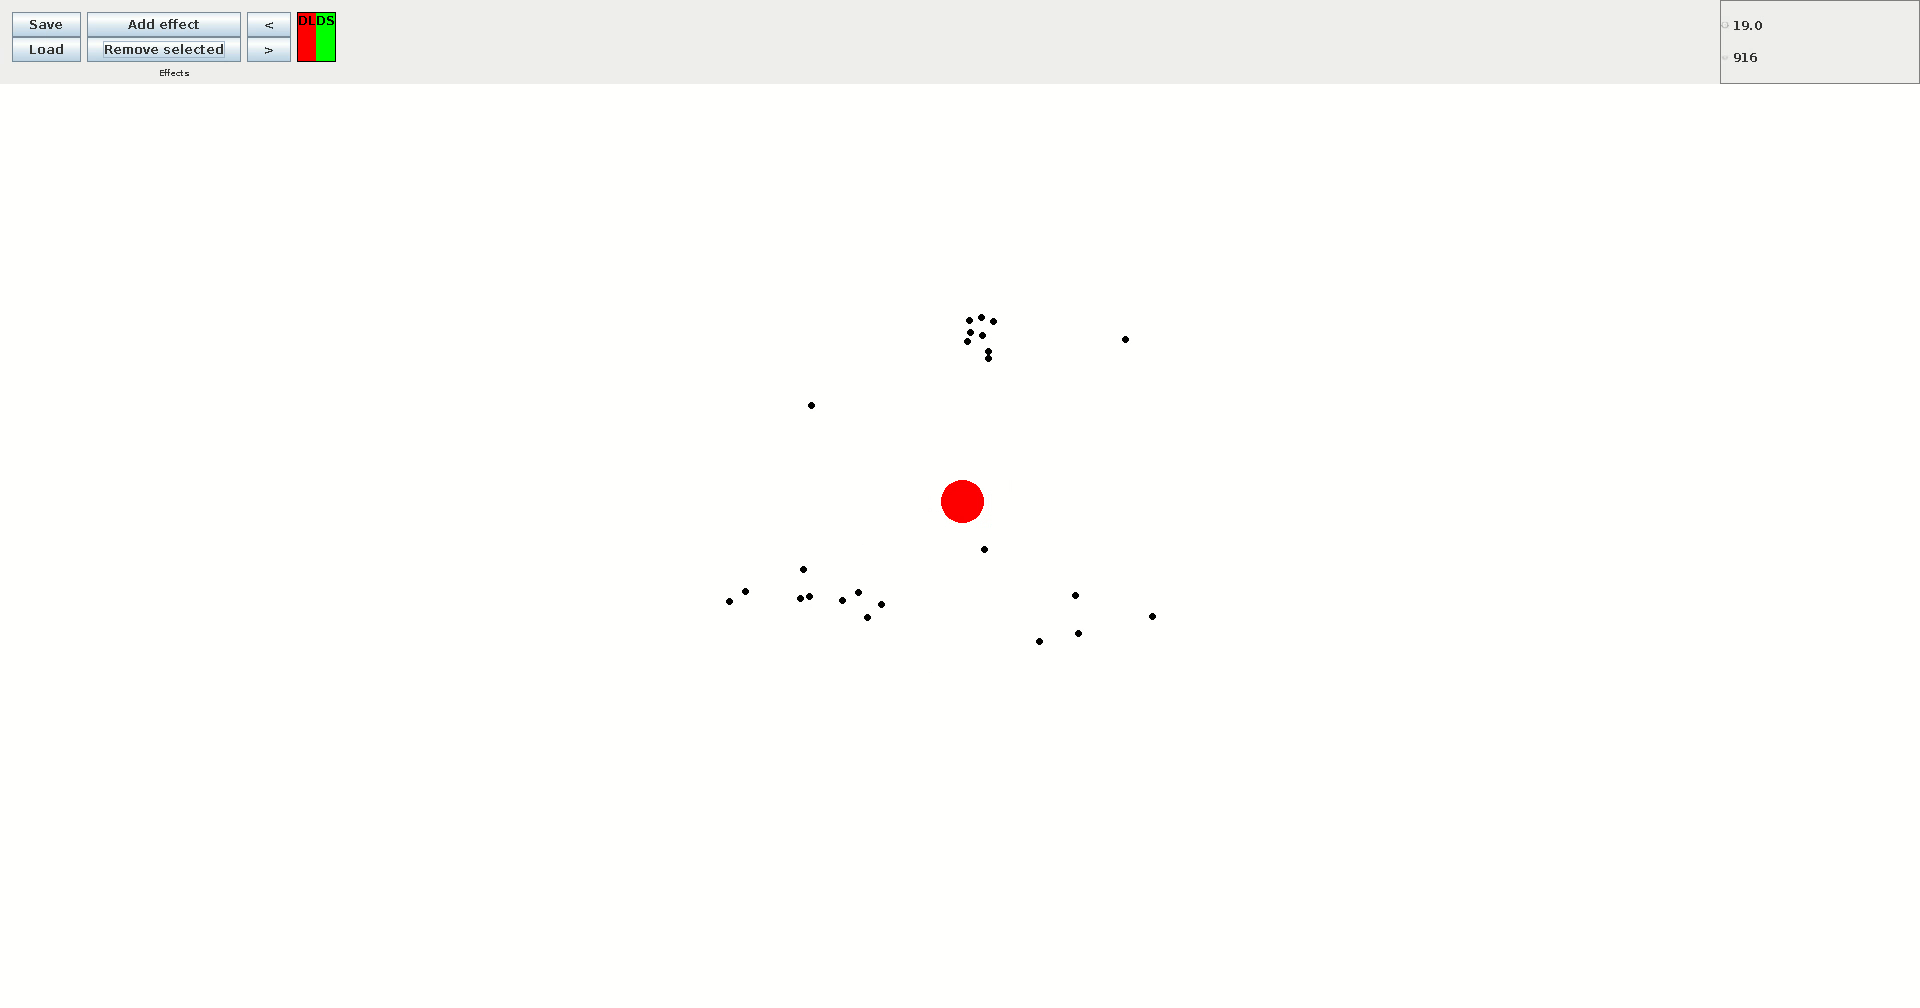
\includegraphics[width=\textwidth]{immagini/casi-studio/influence-with-groups-during.png}
    \end{subfigure}
    \hfill
    \begin{subfigure}[b]{0.75\textwidth}
        \centering
        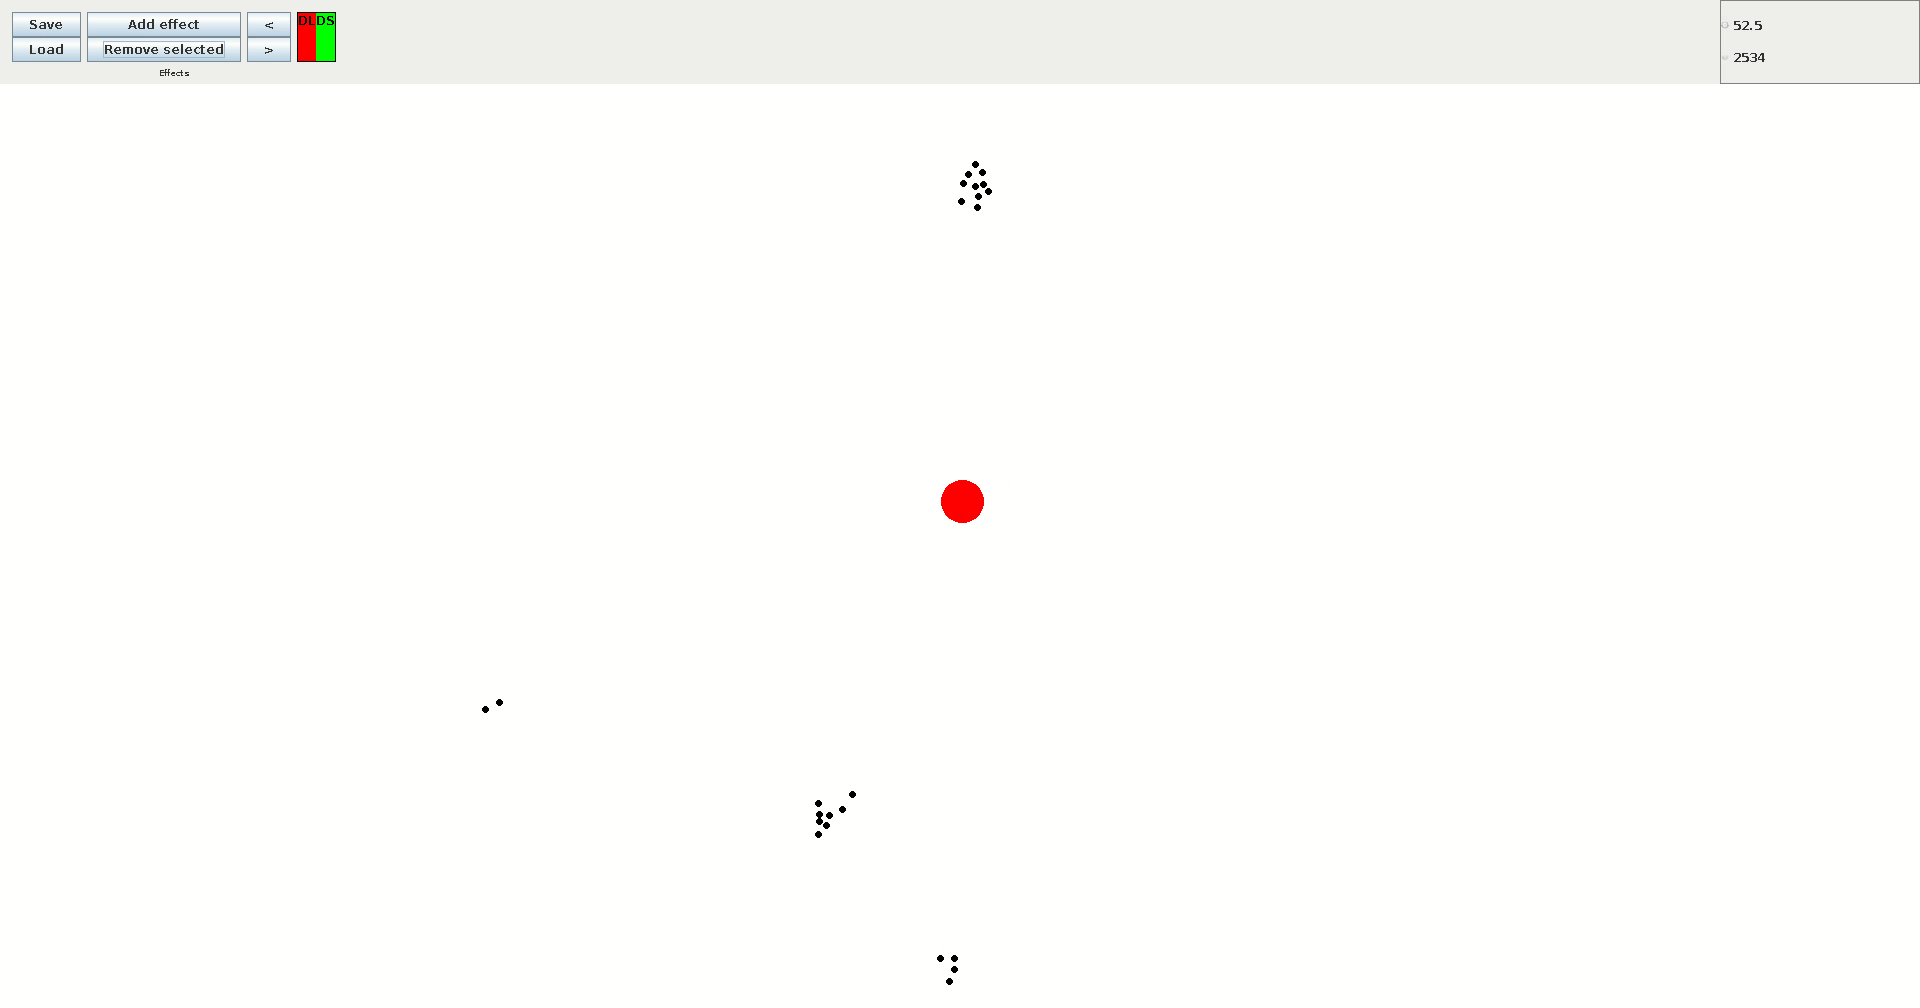
\includegraphics[width=\textwidth]{immagini/casi-studio/influence-with-groups-end.png}
    \end{subfigure}
    \caption{Fotogrammi salienti della simulazione sull'influenza del gruppo considerando quattro insiemi di amici; prima di allontanarsi dalla zona di pericolo, i pedoni cercano di riunirsi con tutti gli altri membri del loro stesso gruppo.}
    \label{fig:influence-with-groups}
\end{figure}
\section{Contagio sociale}
Le scelte di un agente possono riflettere, oltre al proprio, anche lo stato d'animo degli altri soggetti che popolano l'ambiente di interesse. Ogni atteggiamento che scaturisce da una persona può essere, in positivo quanto in negativo, causa della medesima risposta anche in un'altra. \newline
Alla base di questo principio, c'è il già citato meccanismo del contagio sociale, che ha nella trasmissione della paura il suo più lampante esempio. Vedendo un intero gruppo scappare terrorizzato, infatti, la reazione spontanea per un essere umano è quella di fare altrettanto, anche se non si è riscontrata presenza concreta del pericolo.

\subsection{Descrizione della simulazione}
In un ambiente euclideo continuo ed illimitato, vengono definite una zona di sicurezza ed una di pericolo da parti opposte e sono caricati, nello spazio compreso tra esse, due raggruppamenti di pedoni rispettivamente costituiti da 75 e 25 persone. \newline 
Mentre il gruppo più numeroso, costituito da pedoni cognitivi, viene posizionato in prossimità del pericolo, quello meno numeroso è collocato a debita distanza da esso. Nonostante la distanza, la traiettoria da seguire per raggiungere il più velocemente possibile la zona di sicurezza è la stessa per entrambi. \newline
La simulazione è stata eseguita in due casi, differenziando la tipologia di pedone utilizzata per il gruppo da 25: eterogeneo nella prima, cognitivo nella seconda.

\subsection{Risultati ottenuti}
Come è possibile osservare dai momenti significativi raccolti in figura \ref{fig:social-contagion-not-cognitive}, i pedoni eterogenei, trovandosi lontani e non potendo percepire direttamente il pericolo, rimangono al loro posto per tutto il decorrere della simulazione e osservano indifferenti il gruppo costituito dai 75 agenti cognitivi passargli vicino nell'intento di raggiungere la zona di sicurezza. \newline
Diversamente, valutando la situazione negli stessi istanti temporali, ma in presenza di soli agenti cognitivi (figura \ref{fig:social-contagion-cognitive}), possiamo notare come progressivamente anche il secondo gruppo, impaurito dallo stato emotivo dei pedoni del primo, inizi a scappare nella stessa direzione. 

\begin{figure}
    \centering
    \begin{subfigure}[b]{0.75\textwidth}
        \centering
        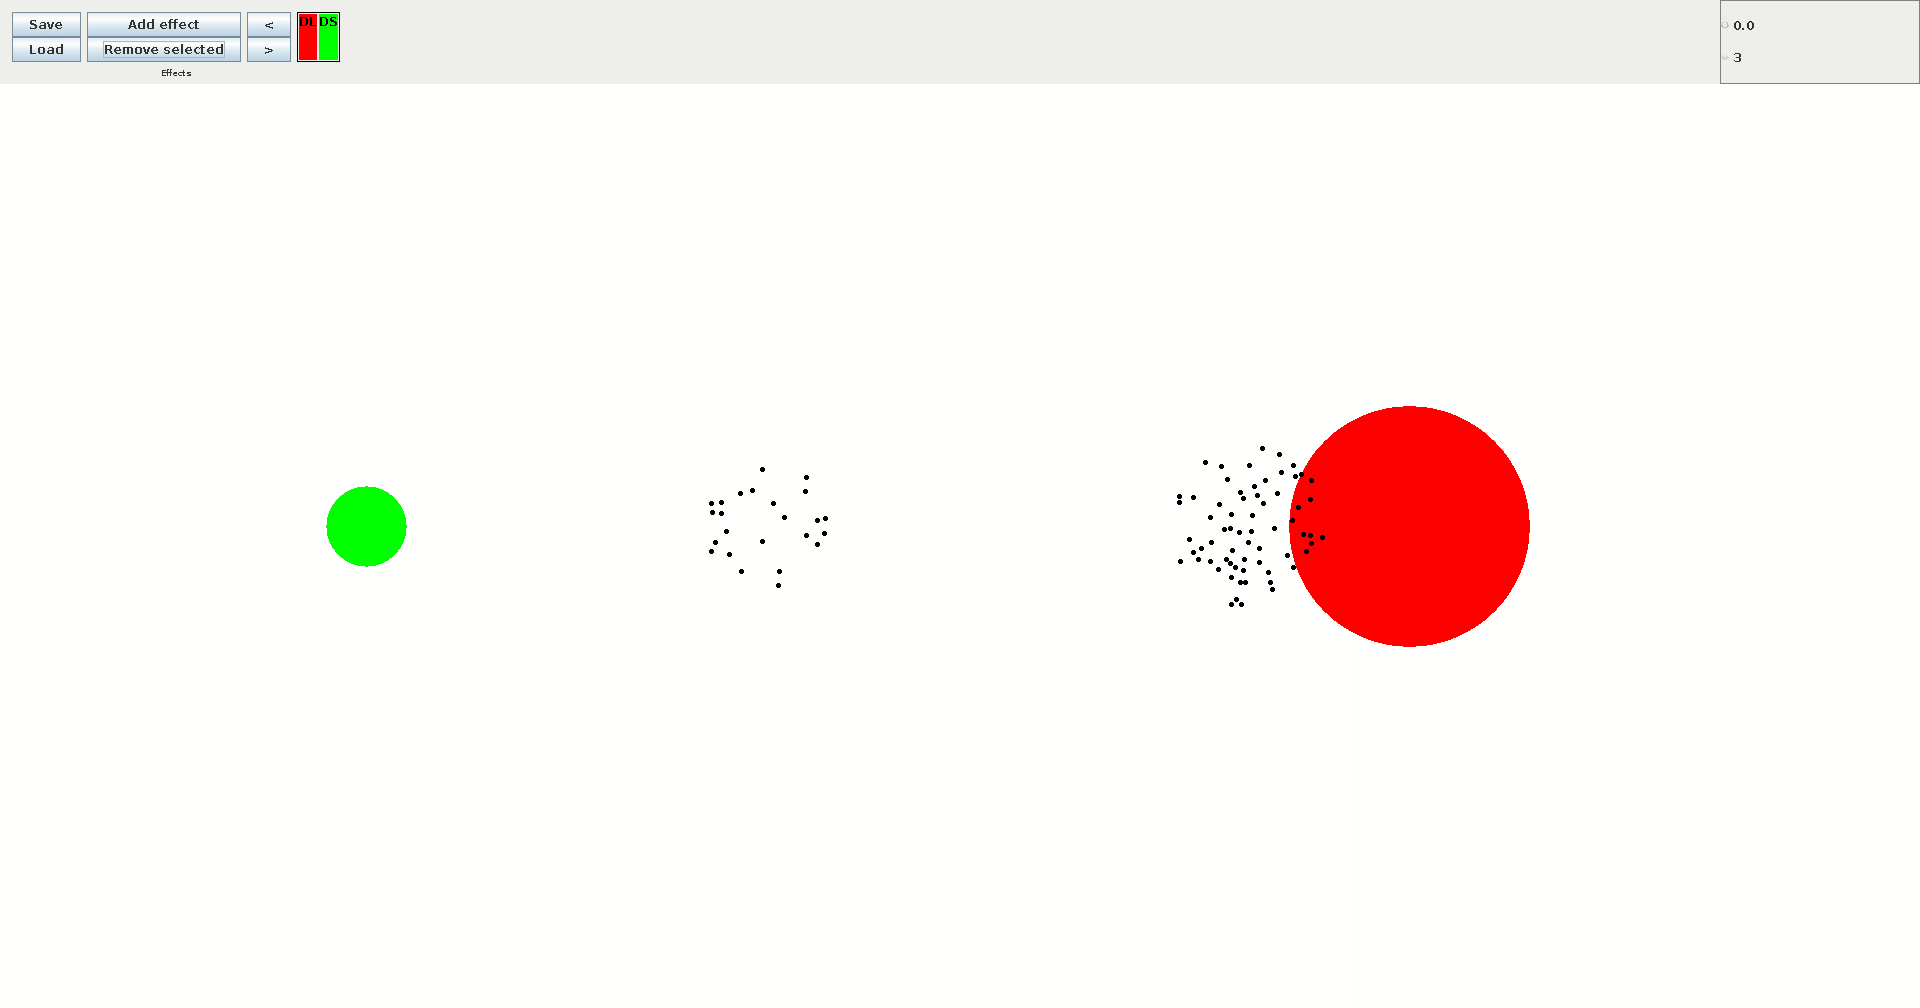
\includegraphics[width=\textwidth]{immagini/casi-studio/social-contagion-not-cognitive-begin.png}
    \end{subfigure}
    \hfill
    \begin{subfigure}[b]{0.75\textwidth}
        \centering
        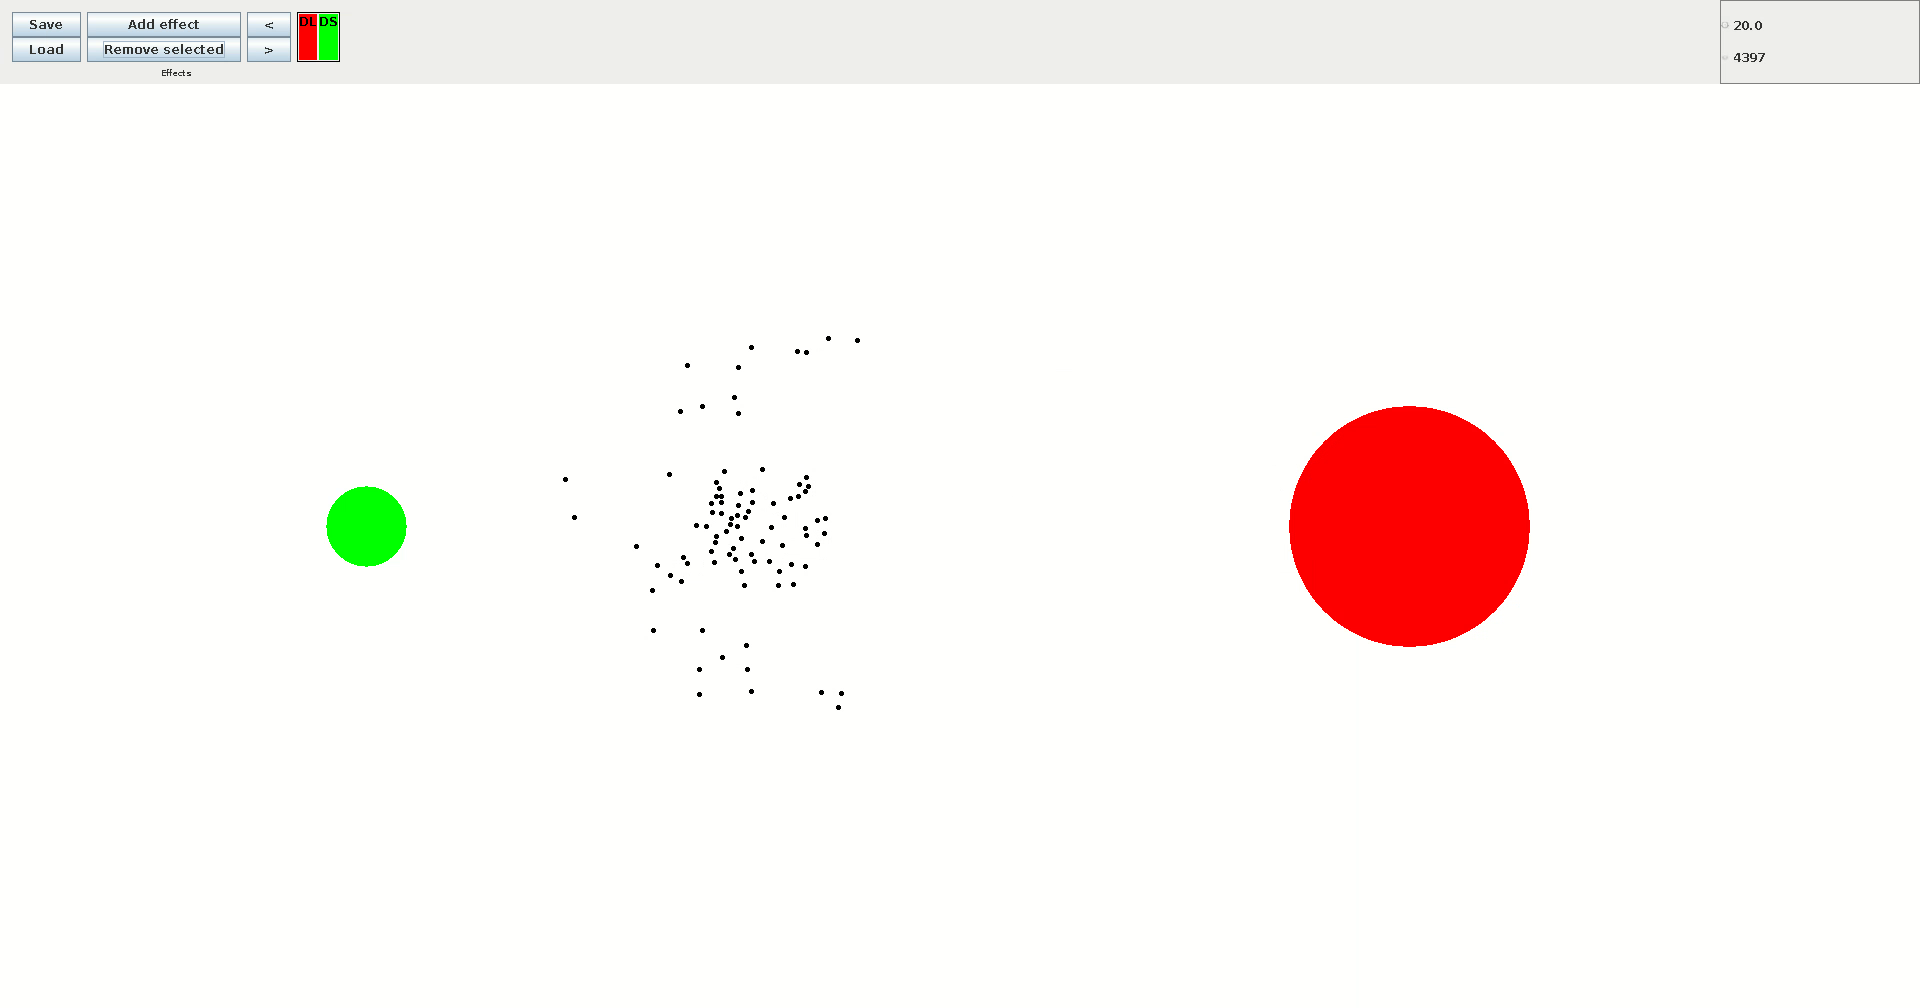
\includegraphics[width=\textwidth]{immagini/casi-studio/social-contagion-not-cognitive-during.png}
    \end{subfigure}
    \hfill
    \begin{subfigure}[b]{0.75\textwidth}
        \centering
        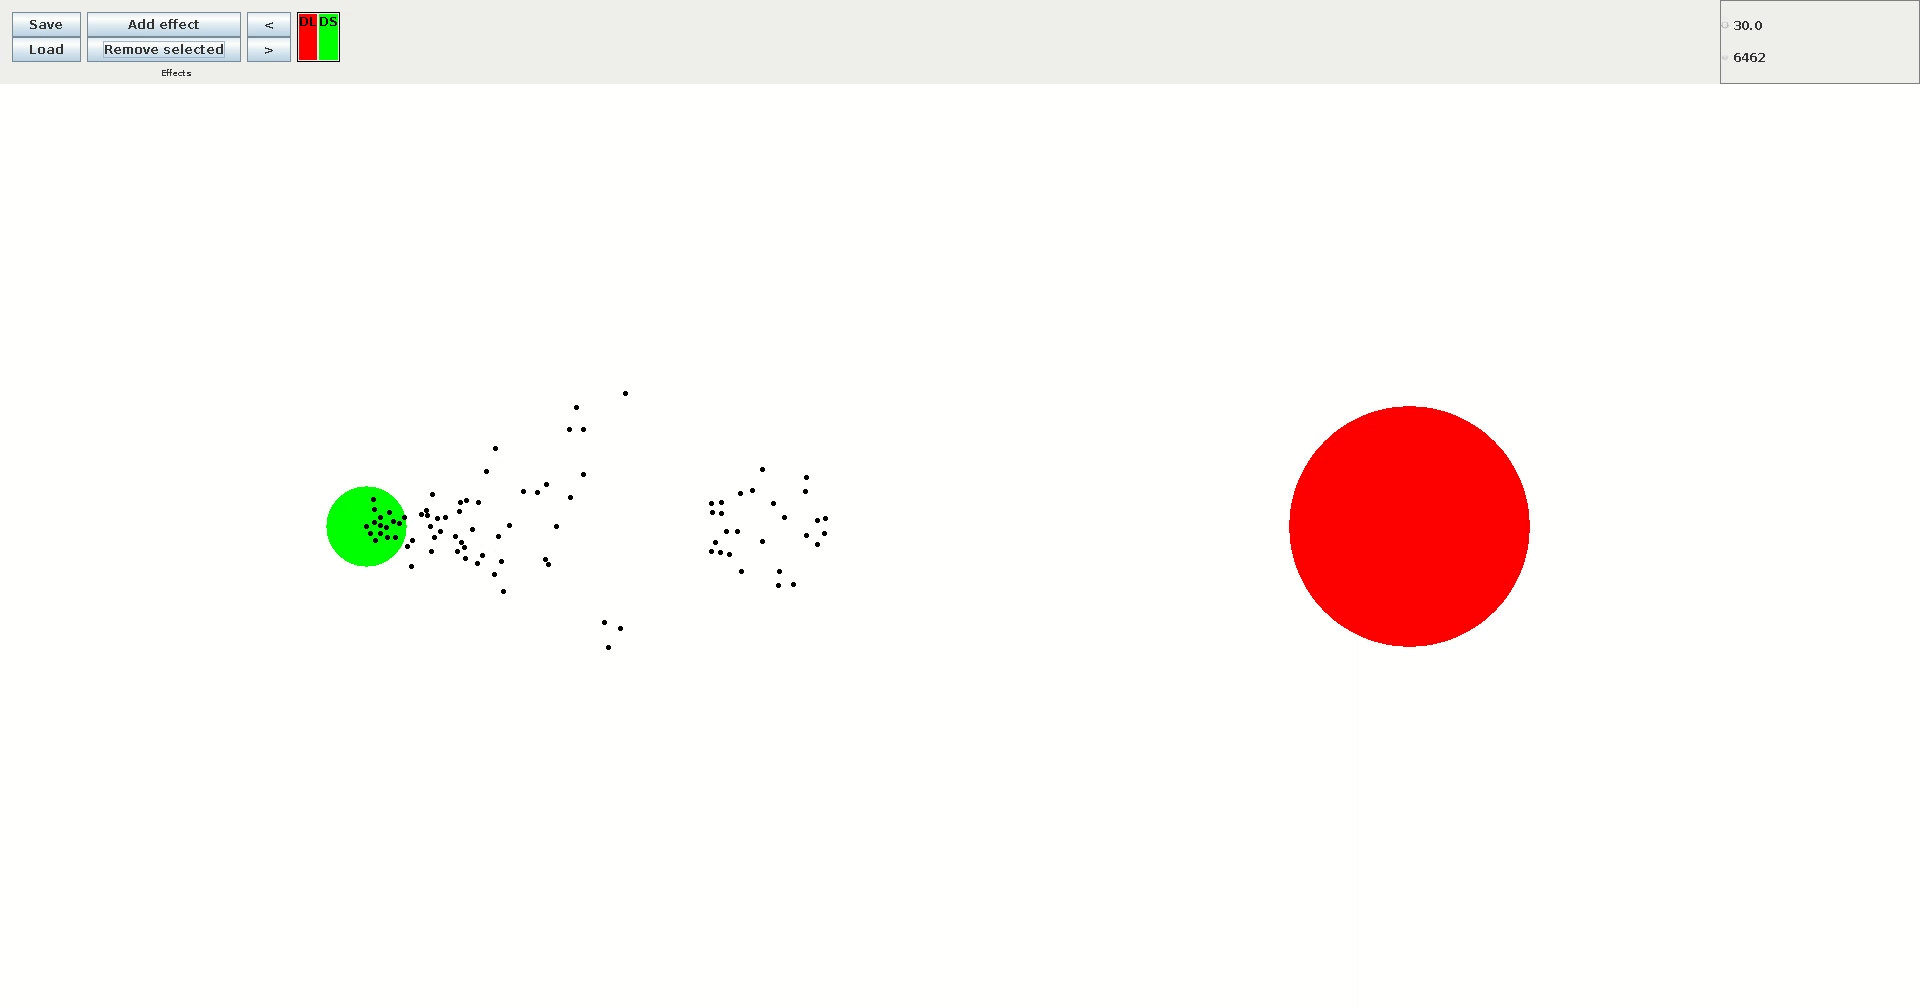
\includegraphics[width=\textwidth]{immagini/casi-studio/social-contagion-not-cognitive-end.png}
    \end{subfigure}
    \caption{Fotogrammi salienti della simulazione sul contagio sociale in presenza di pedoni non cognitivi; non avendo delle caratteristiche emotive e non potendo quindi percepire il panico degli agenti nel gruppo di destra, essi rimangono al loro posto.}
    \label{fig:social-contagion-not-cognitive}
\end{figure}

\begin{figure}
    \centering
    \begin{subfigure}[b]{0.75\textwidth}
        \centering
        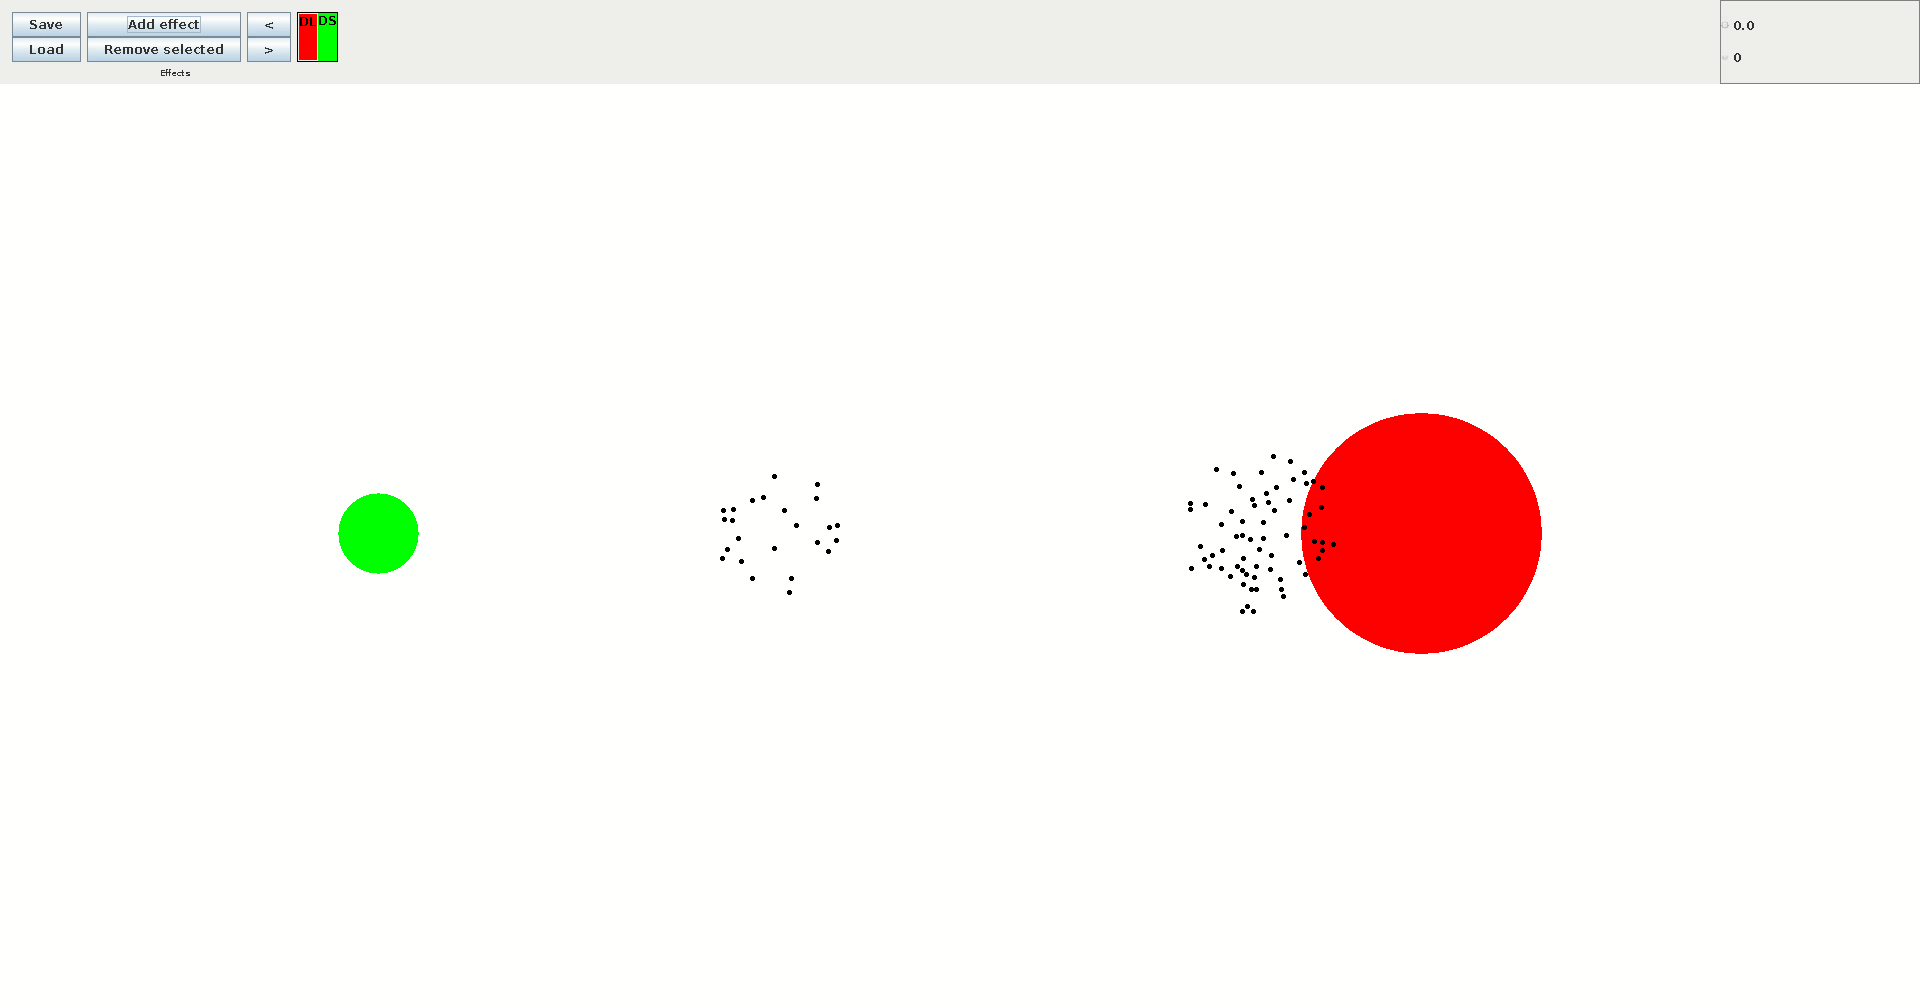
\includegraphics[width=\textwidth]{immagini/casi-studio/social-contagion-cognitive-begin.png}
    \end{subfigure}
    \hfill
    \begin{subfigure}[b]{0.75\textwidth}
        \centering
        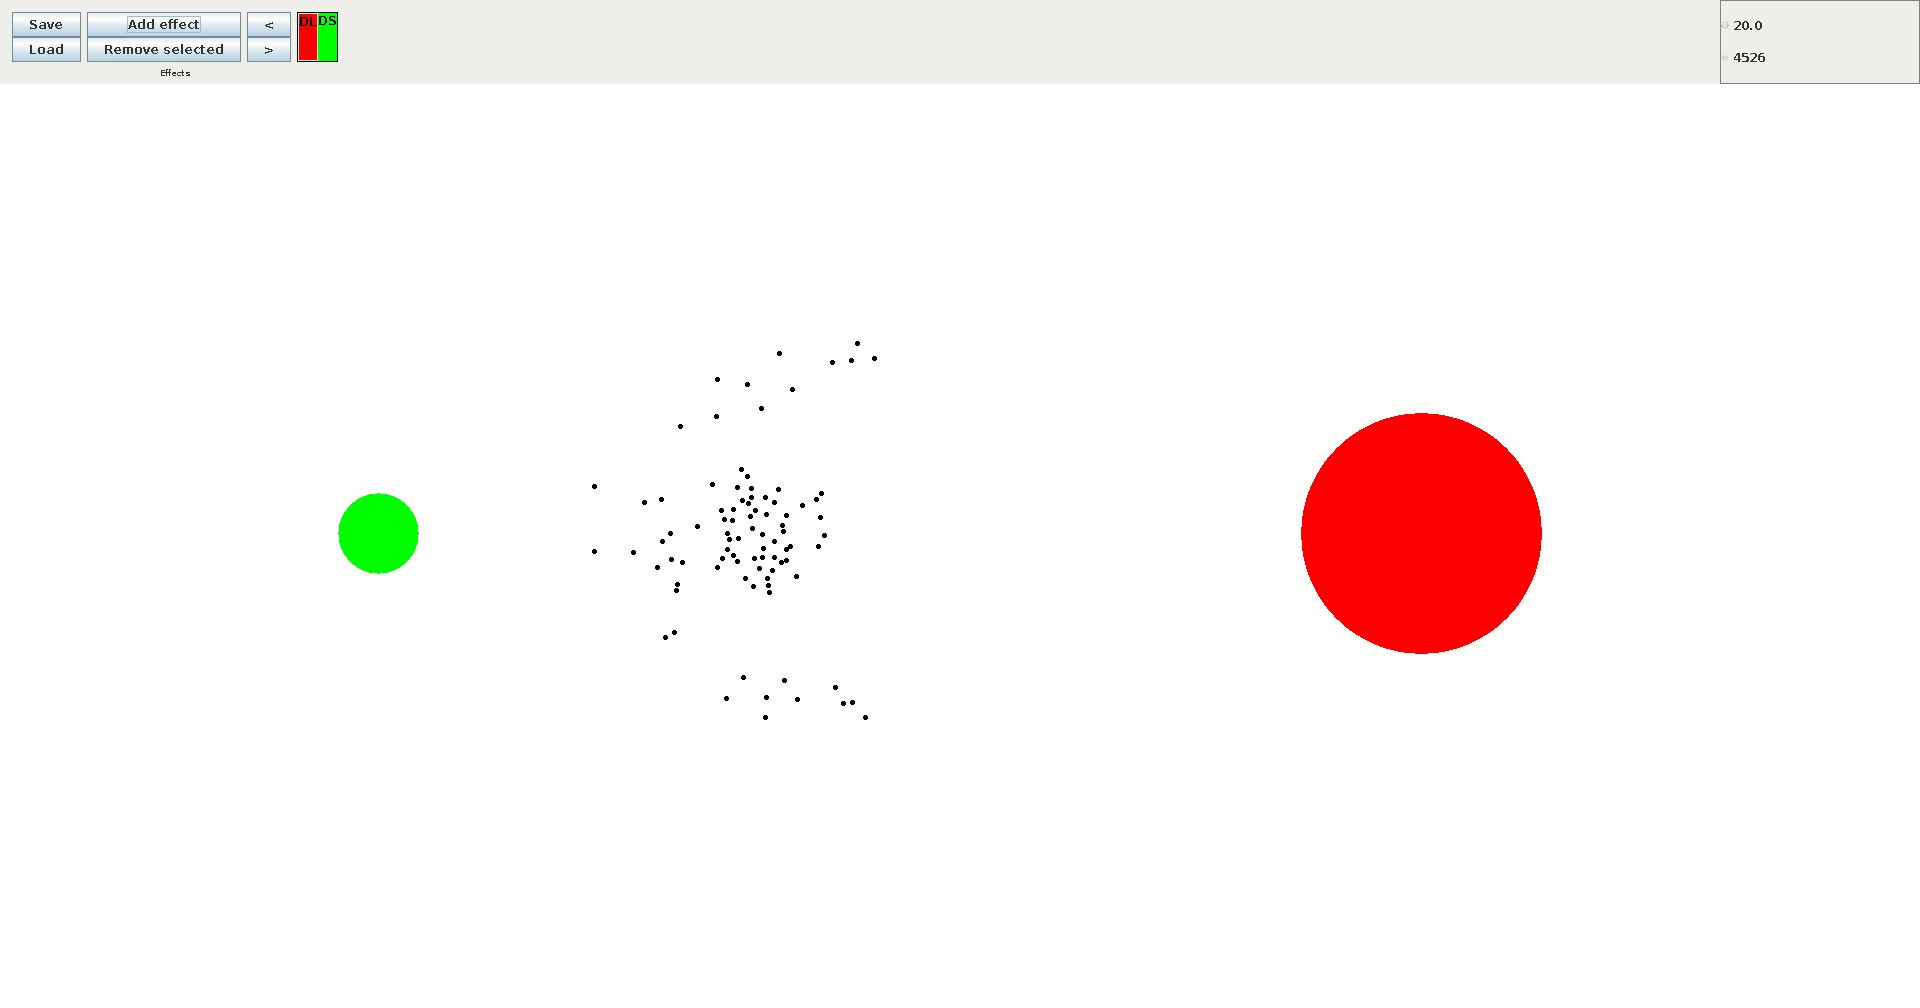
\includegraphics[width=\textwidth]{immagini/casi-studio/social-contagion-cognitive-during.png}
    \end{subfigure}
    \hfill
    \begin{subfigure}[b]{0.75\textwidth}
        \centering
        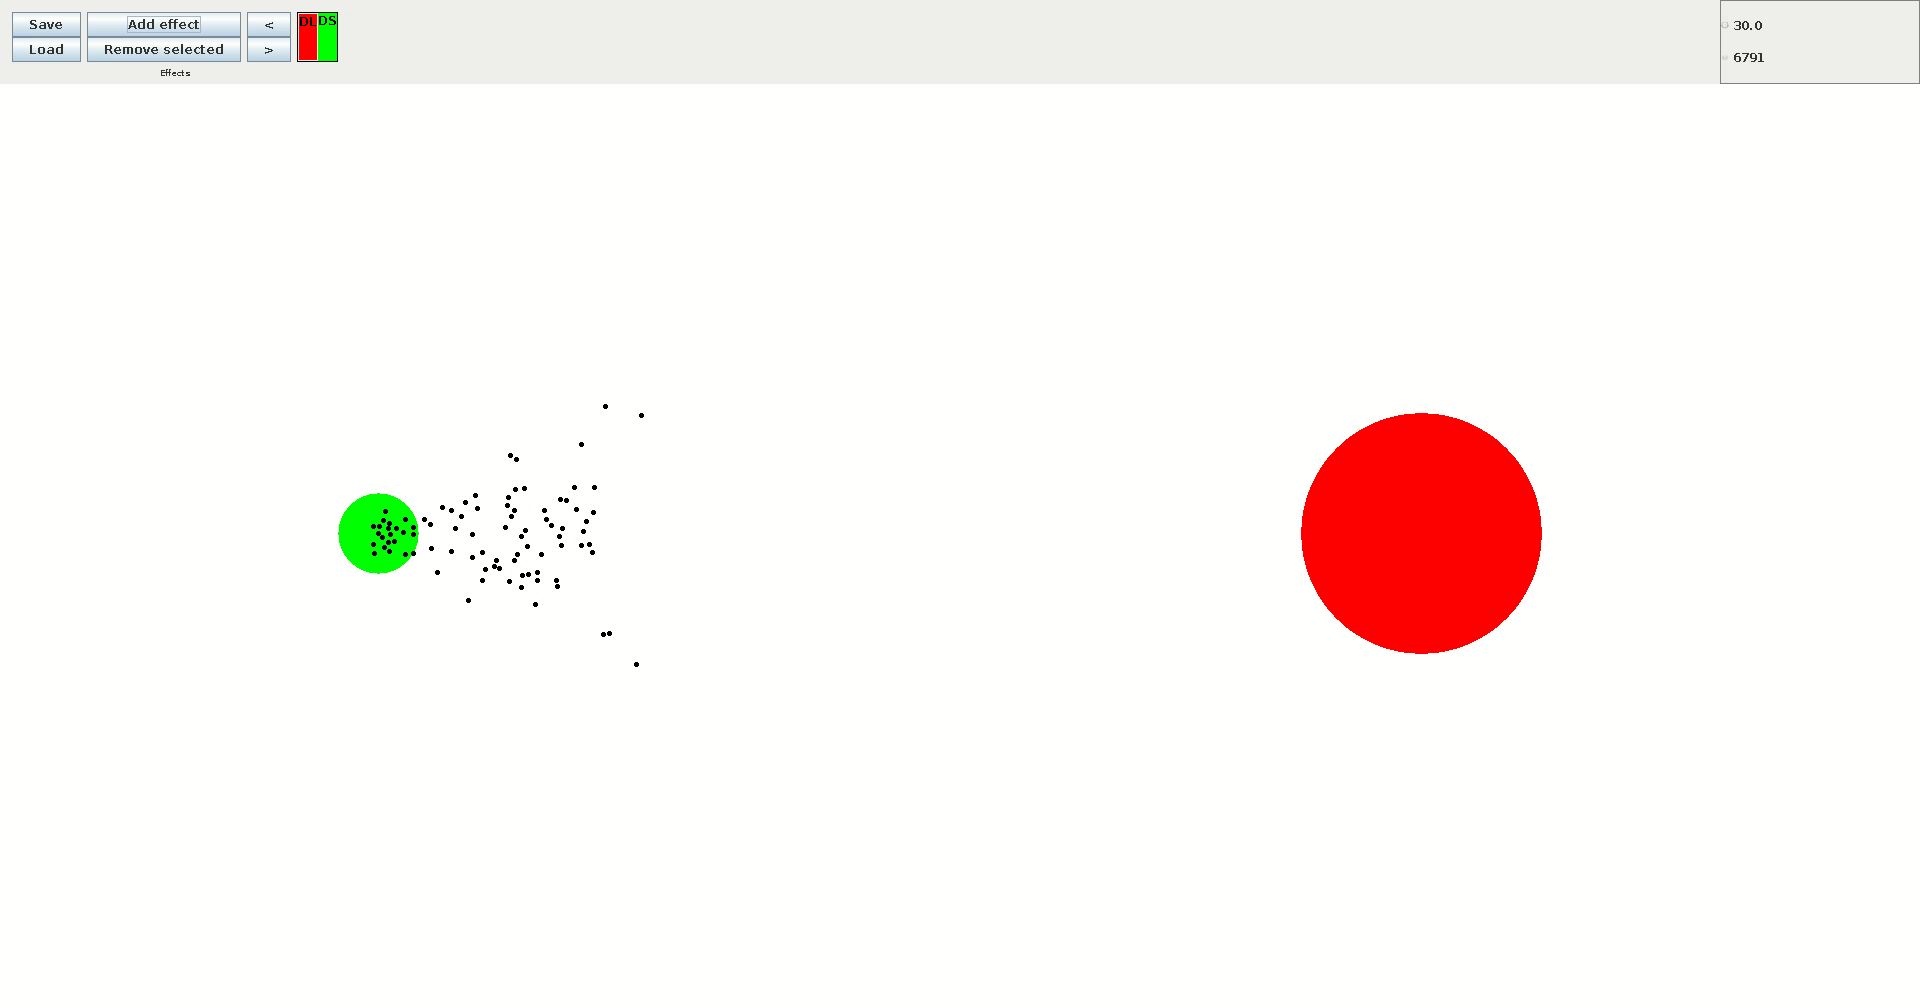
\includegraphics[width=\textwidth]{immagini/casi-studio/social-contagion-cognitive-end.png}
    \end{subfigure}
    \caption{Fotogrammi salienti della simulazione sul contagio sociale in presenza di pedoni cognitivi; il fenomeno della trasmissione del panico nel momento in cui i due gruppi si incrociano, porta gli agenti precedentemente fermi ad iniziare a fuggire.}
    \label{fig:social-contagion-cognitive}
\end{figure}
\section{Scelta dell'uscita}
Un'ambientazione realistica presenta tipicamente molteplici elementi, che contribuiscono ad aumentare la complessità della situazione da analizzare. \newline 
Ad esempio, pensando alla planimetria di un edificio, è inusuale che vi sia una sola uscita, in quanto una scelta del genere comporterebbe problemi sia dal punto di vista logistico sia da quello della sicurezza. \newline
Per determinare i probabili movimenti di una folla in uno scenario contraddistinto da più punti di interesse aventi lo stesso scopo, è necessario scegliere con cura la strategia da utilizzare per la combinazione delle varie forze in gioco, altrimenti si rischia di ottenere simulazioni poco attendibili.

\subsection{Descrizione della simulazione}
Lo scenario utilizzato è molto simile a quello impiegato nelle simulazioni del modello IMPACT: un ambiente limitato di dimensione quadrata con quattro uscite, al centro del quale è presente una zona di pericolo. Intorno ad essa, sono disposti casualmente 150 agenti cognitivi. \newline
In questo caso, non è possibile definire univocamente il movimento dei vari pedoni, in quanto, essendo presenti multiple uscite, non tutti hanno in comune lo stesso punto di arrivo. \newline
La stessa simulazione è stata ripetuta prima considerando come reazione responsabile del movimento il \texttt{BlendedSteering}, che utilizza la strategia basata sulla distanza, poi il \texttt{PrioritySteering}, che utilizza la strategia basata sulla massima vicinanza.

\subsection{Risultati ottenuti}
I momenti salienti in figura \ref{fig:multiple-exits-blended} dimostrano come l'utilizzo del \texttt{BlendedSteering} non sia adatto a descrivere la situazione e conduca a risultati inverosimili, dovuti al fatto che il pedone rimane perennemente indeciso su quale uscita scegliere in maniera particolare se si trova al centro della stanza, che è il luogo da cui dovrebbe avere più interesse a stare lontano. \newline
Ben diverso è il risultato nel caso si utilizzi il \texttt{PrioritySteering} (figura \ref{fig:multiple-exits-priority}), che determina un comportamento più simile a quello che si osserverebbe nella vita reale, contraddistinto da un iniziale allontanamento dal pericolo seguito dal raggiungimento dell'uscita più vicina.

\begin{figure}
    \centering
    \begin{subfigure}[b]{0.75\textwidth}
        \centering
        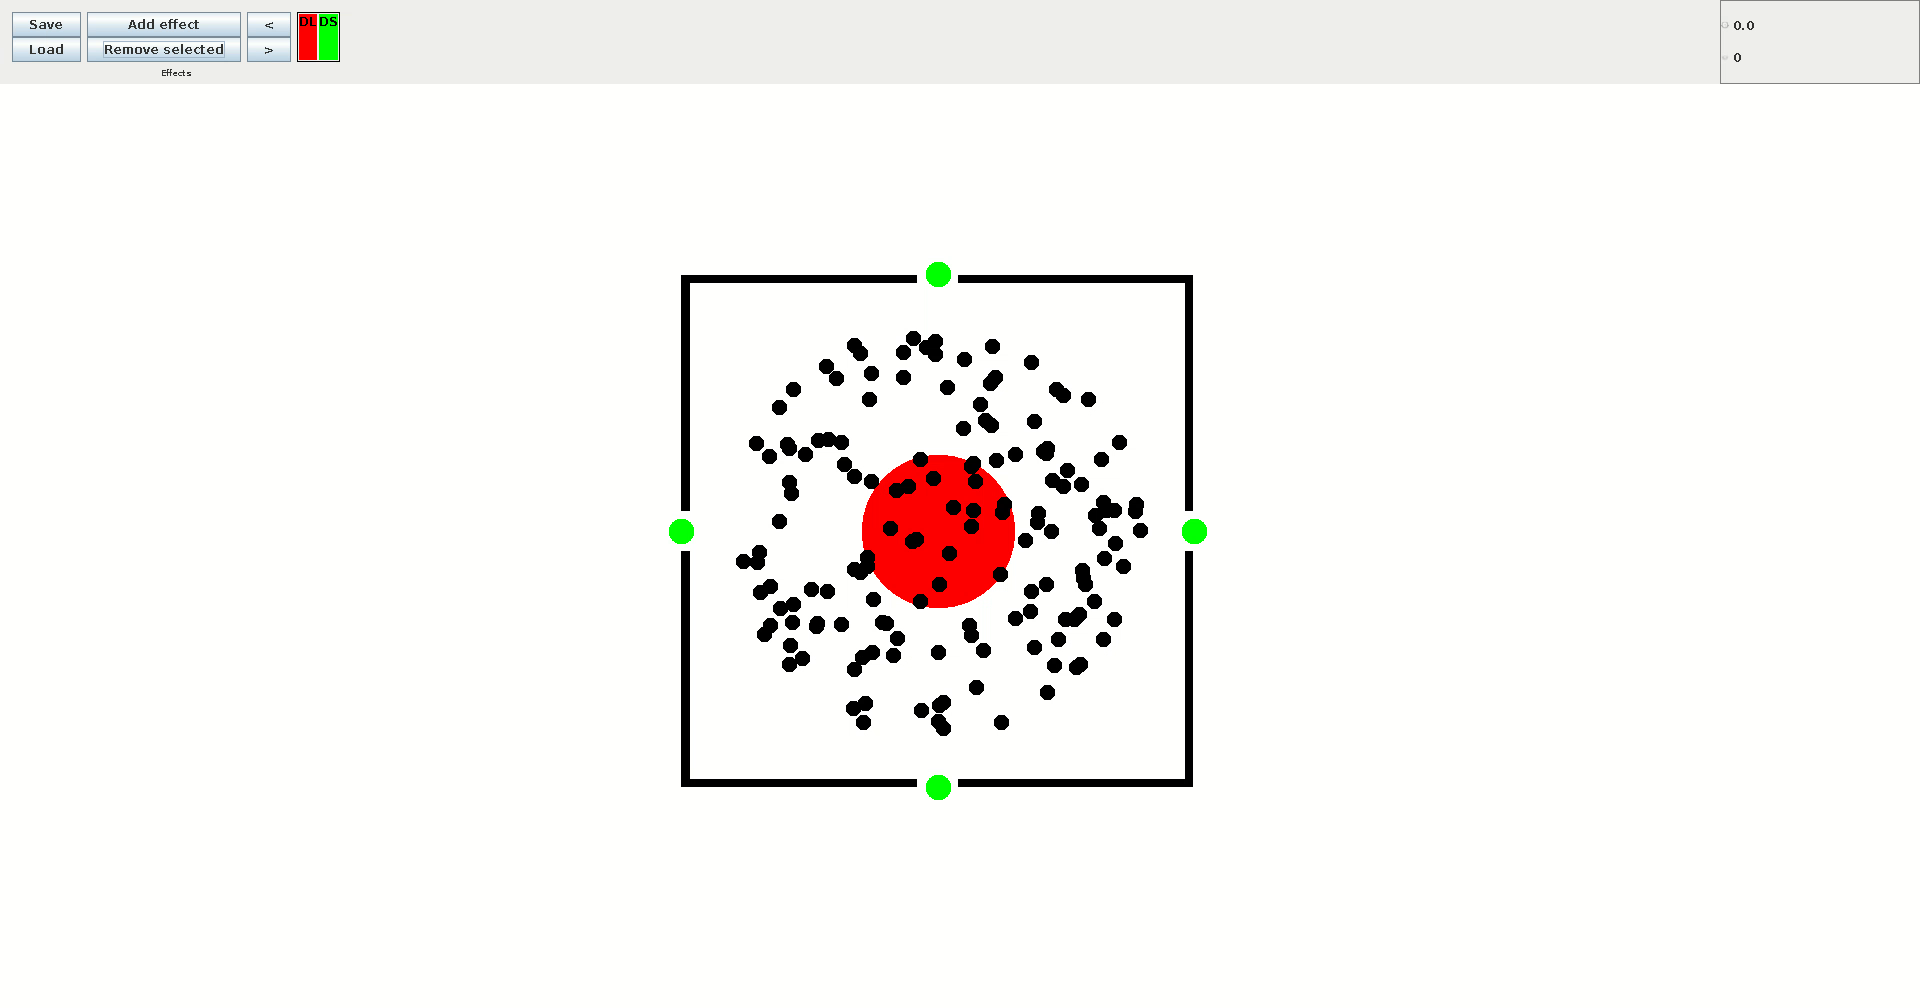
\includegraphics[width=\textwidth]{immagini/casi-studio/multiple-exits-blended-begin.png}
    \end{subfigure}
    \hfill
    \begin{subfigure}[b]{0.75\textwidth}
        \centering
        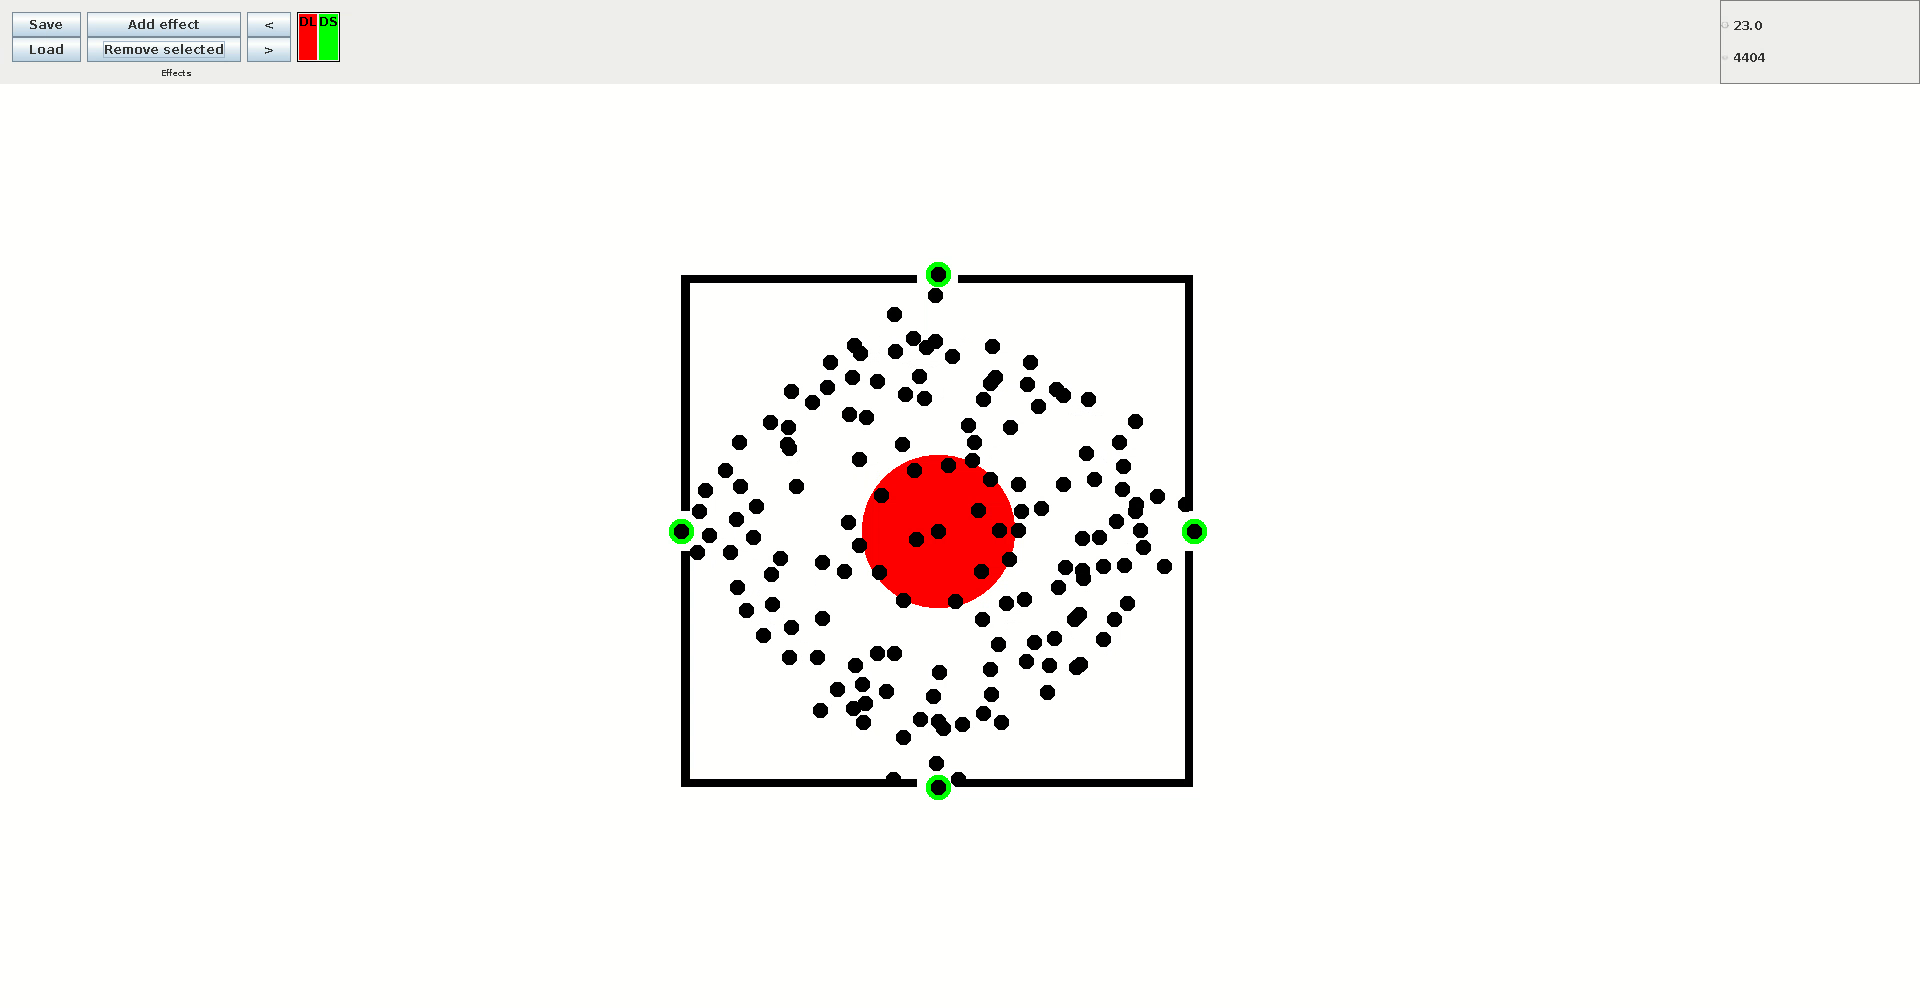
\includegraphics[width=\textwidth]{immagini/casi-studio/multiple-exits-blended-during.png}
    \end{subfigure}
    \hfill
    \begin{subfigure}[b]{0.75\textwidth}
        \centering
        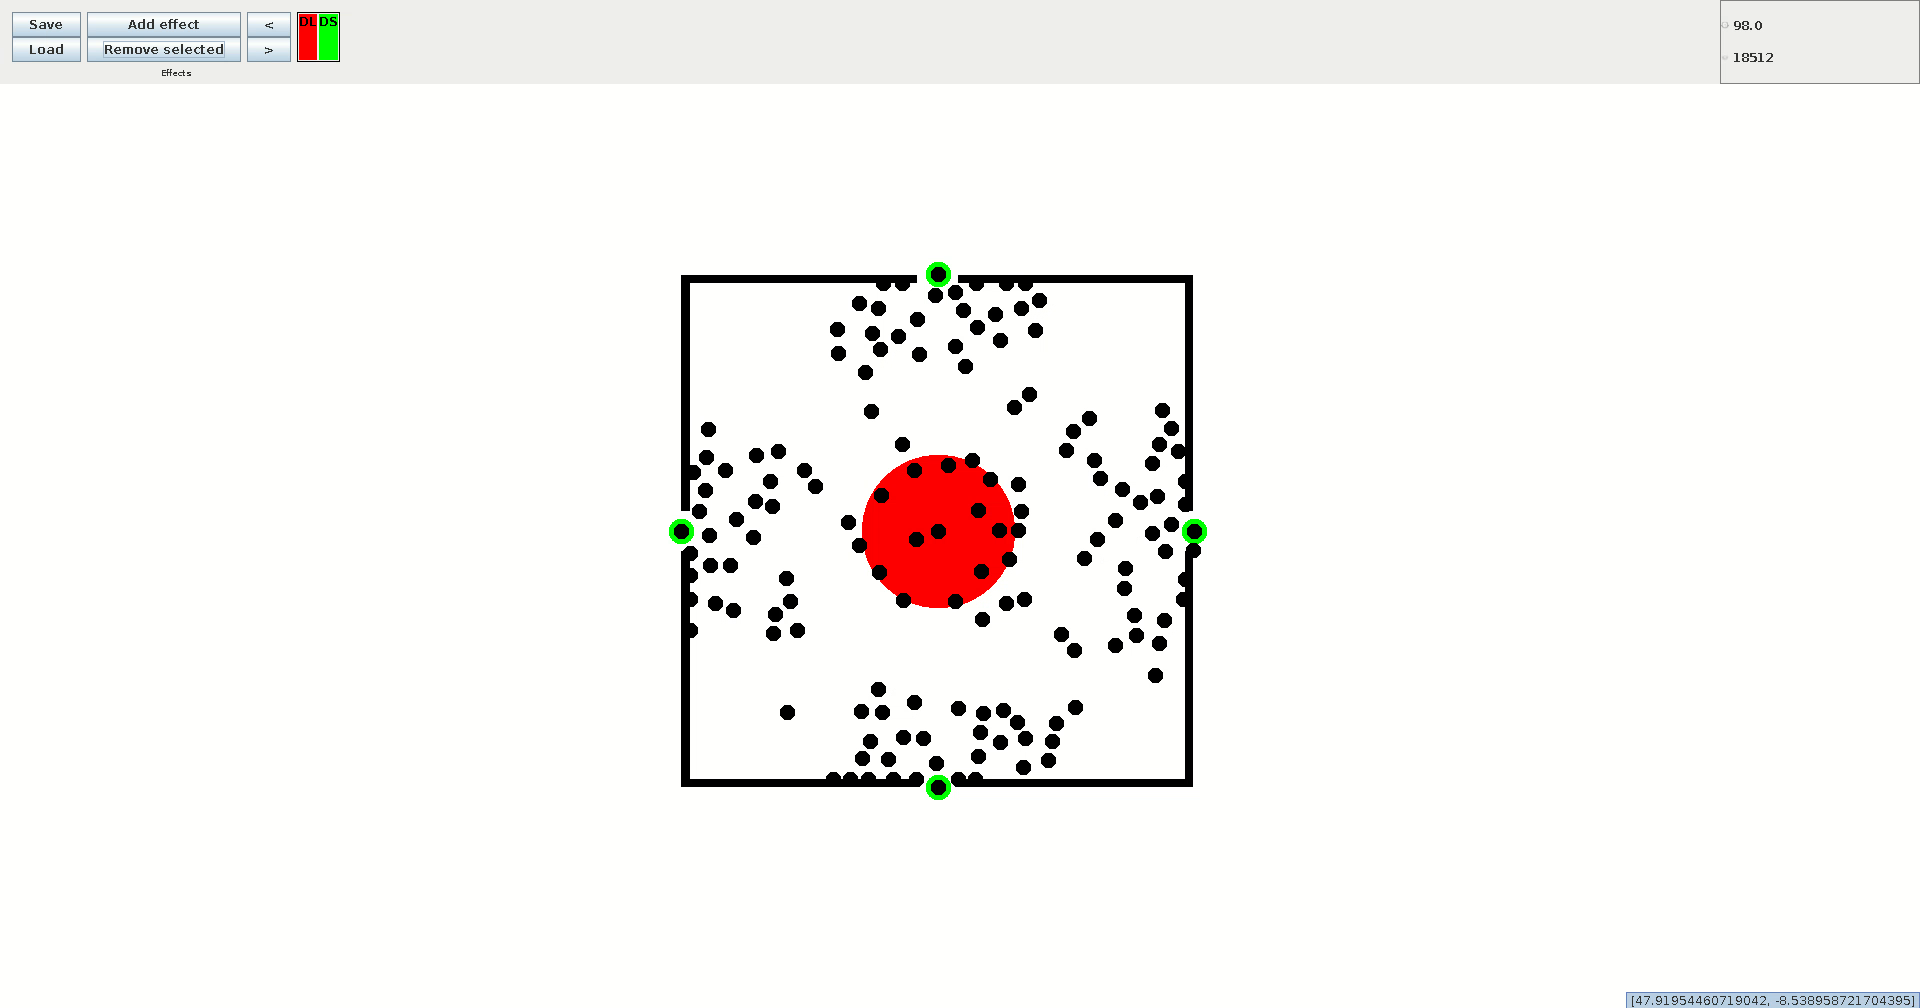
\includegraphics[width=\textwidth]{immagini/casi-studio/multiple-exits-blended-end.png}
    \end{subfigure}
    \caption{Fotogrammi salienti della simulazione sulla scelta dell'uscita utilizzando come strategia il \texttt{BlendedSteering}; le molteplici direzioni che il pedone è portato a seguire dai vari comportamenti di steering conducono a risultati inverosimili.}
    \label{fig:multiple-exits-blended}
\end{figure}

\begin{figure}
    \centering
    \begin{subfigure}[b]{0.75\textwidth}
        \centering
        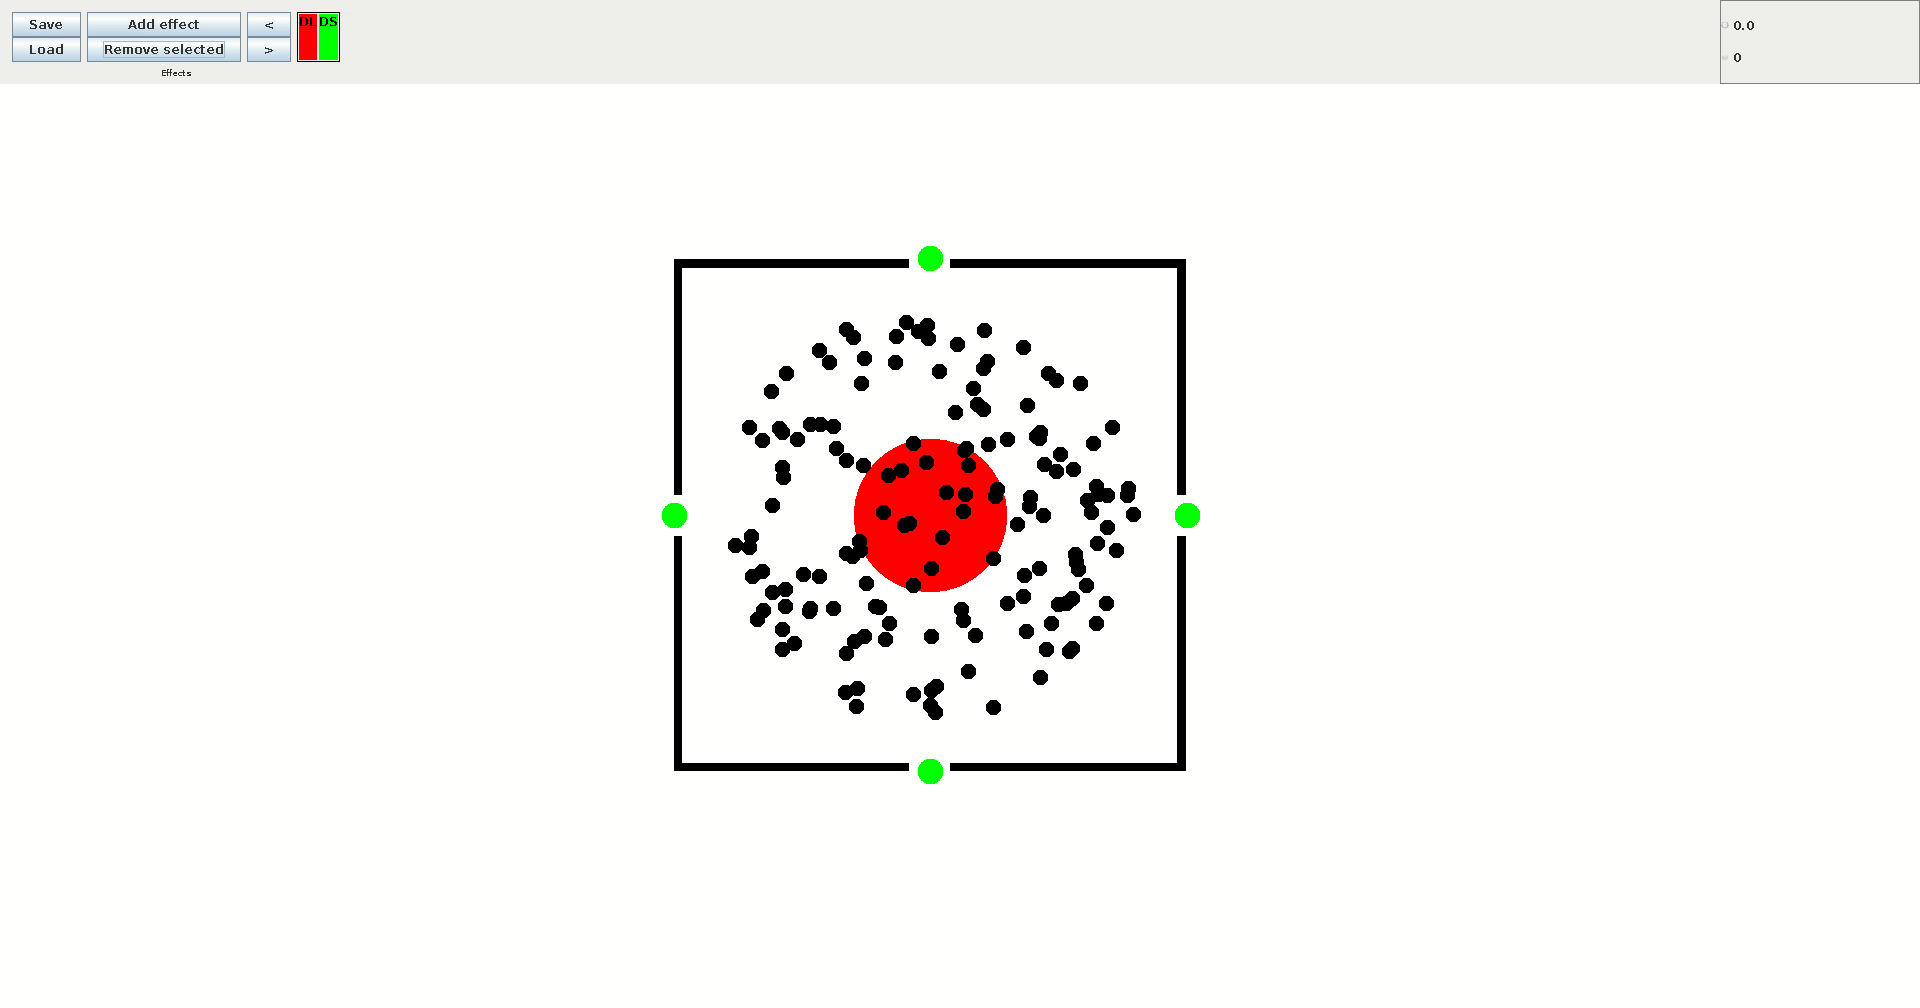
\includegraphics[width=\textwidth]{immagini/casi-studio/multiple-exits-priority-begin.png}
    \end{subfigure}
    \hfill
    \begin{subfigure}[b]{0.75\textwidth}
        \centering
        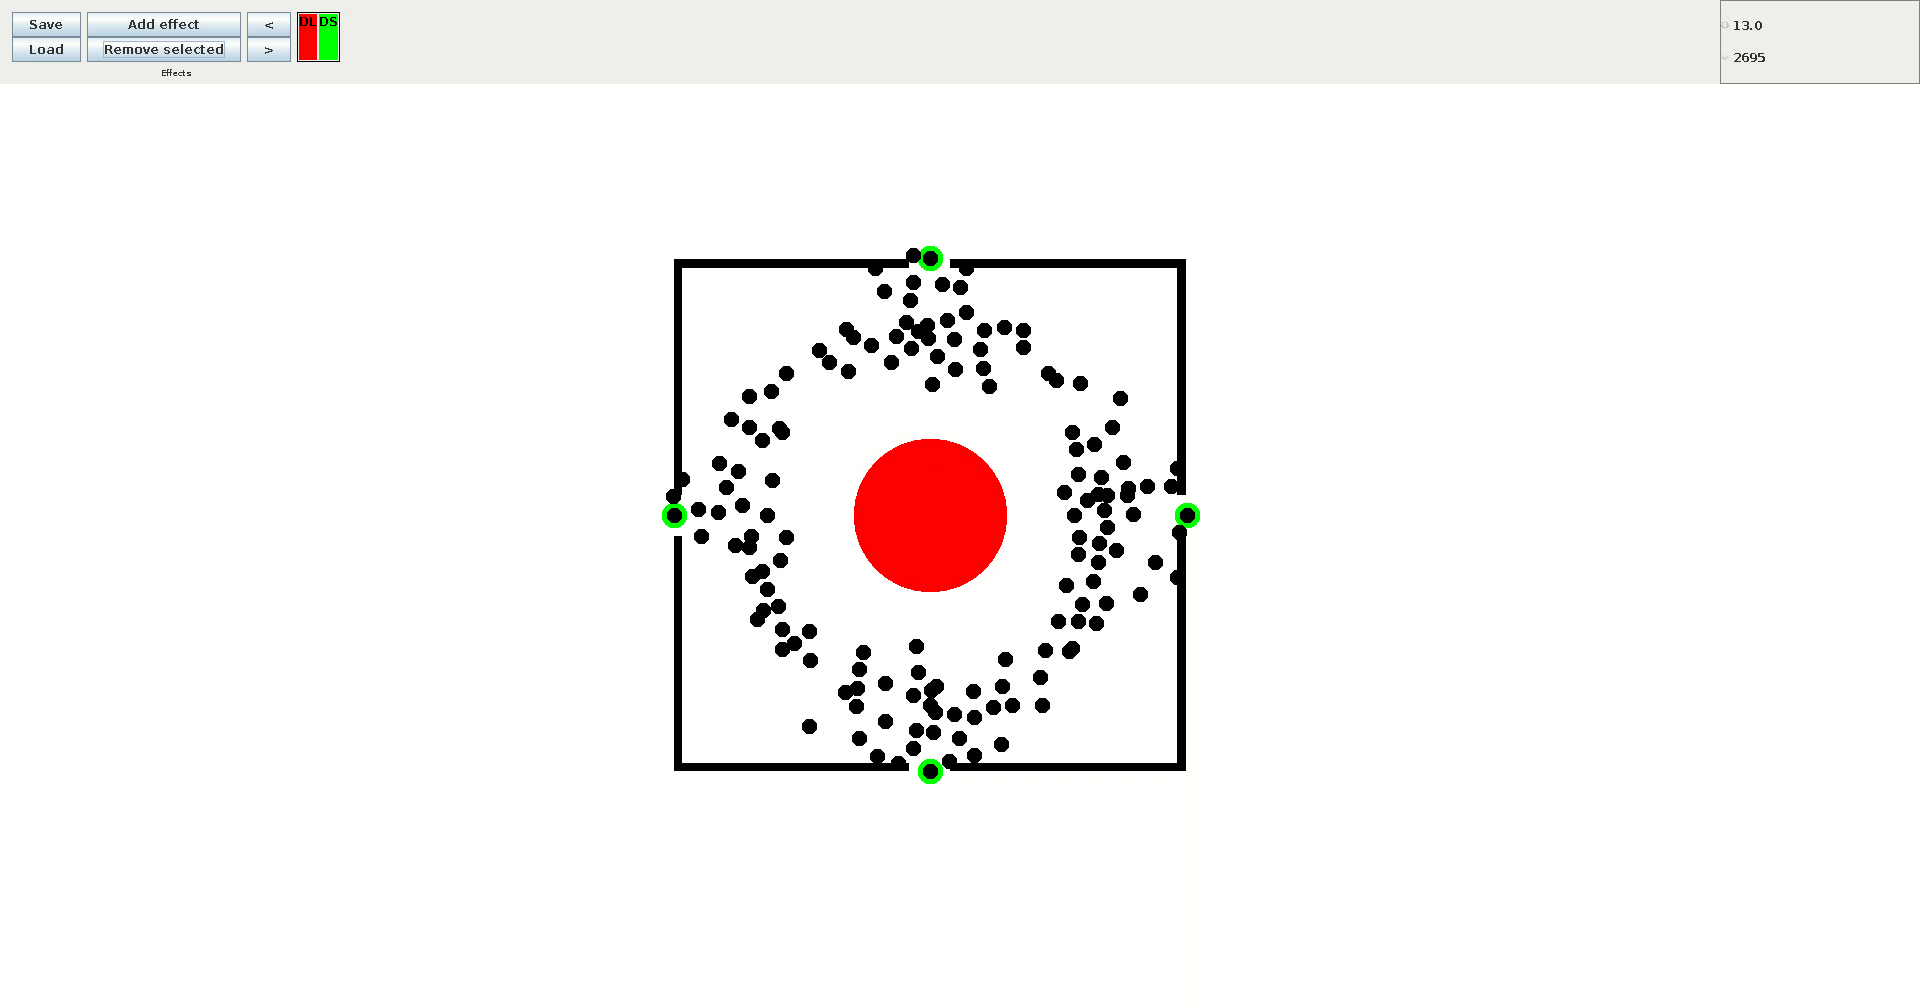
\includegraphics[width=\textwidth]{immagini/casi-studio/multiple-exits-priority-during.png}
    \end{subfigure}
    \hfill
    \begin{subfigure}[b]{0.75\textwidth}
        \centering
        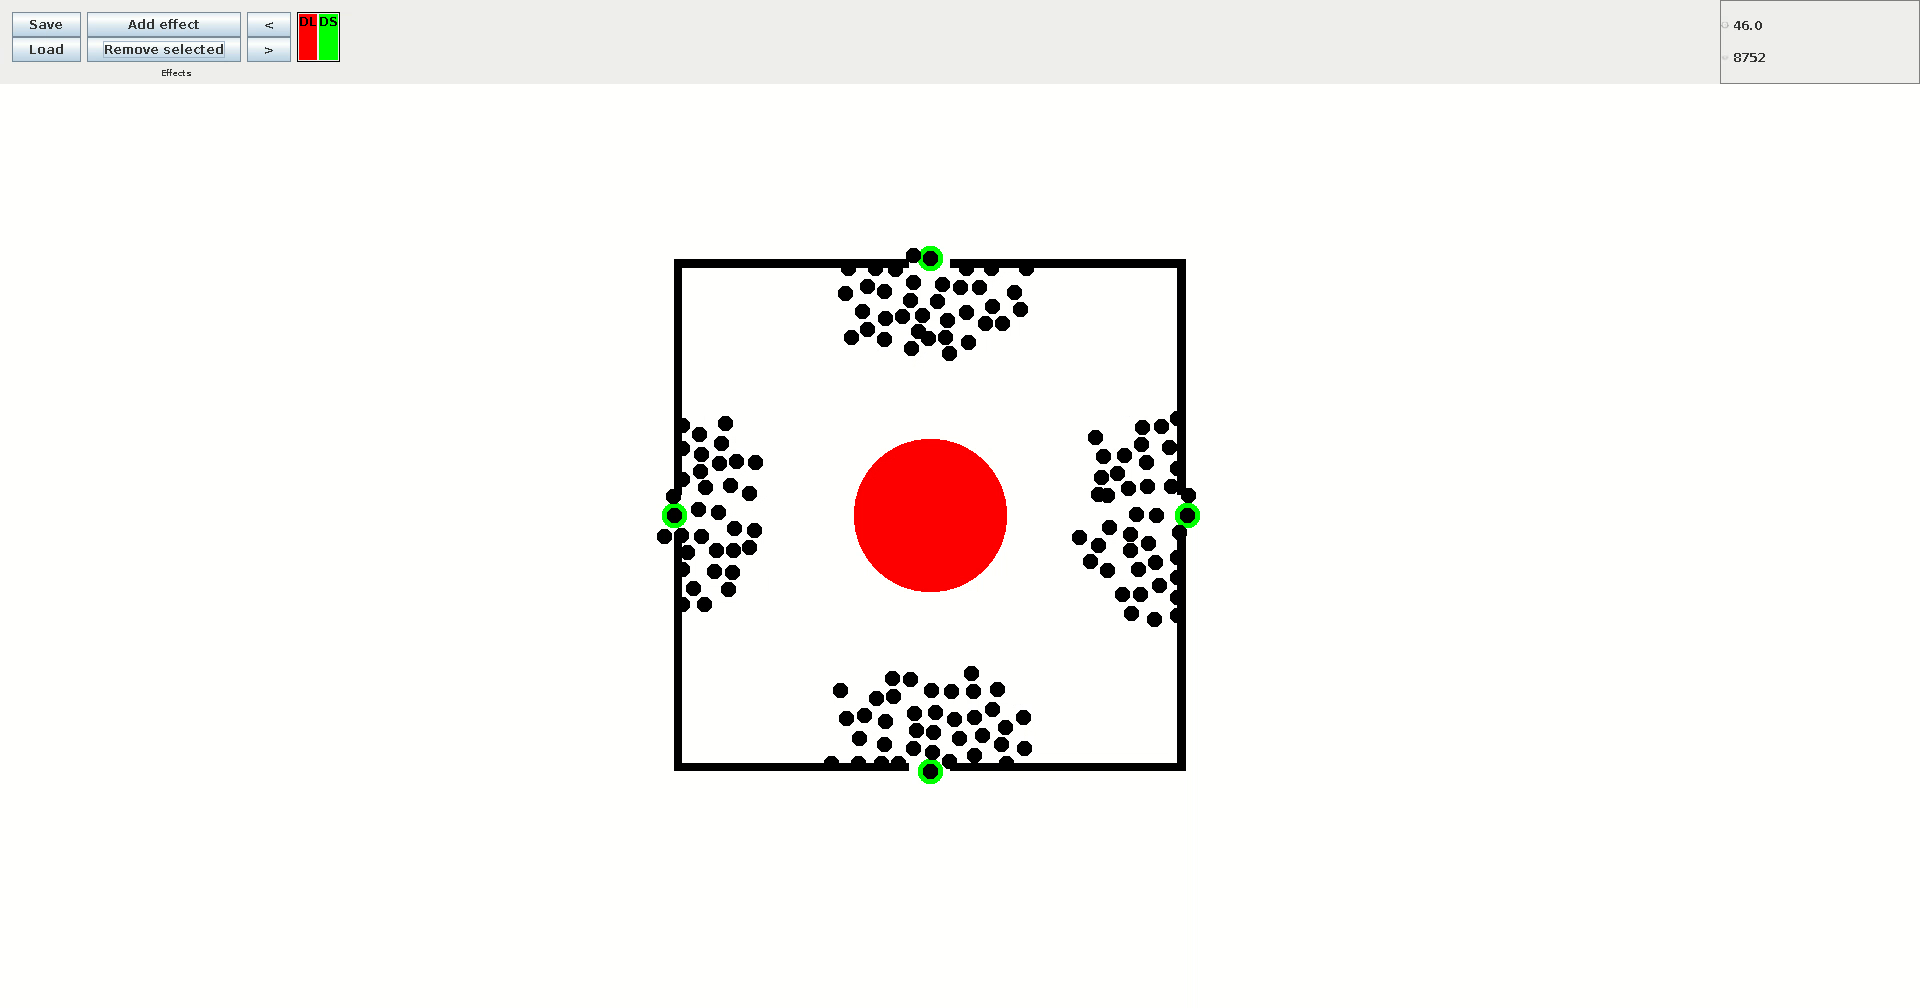
\includegraphics[width=\textwidth]{immagini/casi-studio/multiple-exits-priority-end.png}
    \end{subfigure}
    \caption{Fotogrammi salienti della simulazione sulla scelta dell'uscita utilizzando come strategia il \texttt{PrioritySteering}; definendo una priorità tra le azioni da eseguire, è possibile condurre i pedoni verso l'uscita loro più congeniale.}
    \label{fig:multiple-exits-priority}
\end{figure}
\section{Presenza di ostacoli}
Gli ambienti visti fino ad ora non presentano alcun tipo di ostacolo, quindi un nodo è vincolato nel movimento solo dalla presenza nelle sue vicinanze di eventuali altri suoi simili. \newline
Per descrivere in maniera più dettagliata uno scenario, è necessario considerare anche la presenza di oggetti al suo interno, che in relazione alla loro grandezza e alla loro posizione possono incidere significativamente sui tempi necessari ad un pedone per scappare o raggiungere una determinata zona.

\subsection{Descrizione della simulazione}
Grazie all'uso dell'\texttt{ImageEnvironment} è stato possibile definire un ambiente contenente cinque ostacoli: quattro rettangolari rispettivamente in alto, in basso, a destra e a sinistra della scena ed uno circolare al centro di essa. \newline
Si è pensato di collocare tre insiemi di pedoni nelle vicinanze di questi oggetti e di definire una zona di sicurezza comune, avendo cura che vi fosse almeno un elemento di intralcio tra essa ed un qualsiasi agente. \newline
La simulazione è stata eseguita prima non considerando il comportamento di steering dell'aggiramento degli ostacoli, poi inserendolo tra le azioni.

\subsection{Risultati ottenuti}
Mentre nella prima simulazione molti nodi rimangono attaccati agli ostacoli, nel vano tentativo di volerci passare attraverso per raggiungere la zona di loro interesse (figura \ref{fig:no-obstacle-avoidance}), nella seconda tutti i pedoni riescono ad arrivare a destinazione, schivando i vari oggetti nella direzione loro più congeniale in relazione alla posizione da cui erano partiti. Il tragitto percorso è deducibile dalla figura \ref{fig:obstacle-avoidance}.

\begin{figure}
    \centering
    \begin{subfigure}[b]{0.75\textwidth}
        \centering
        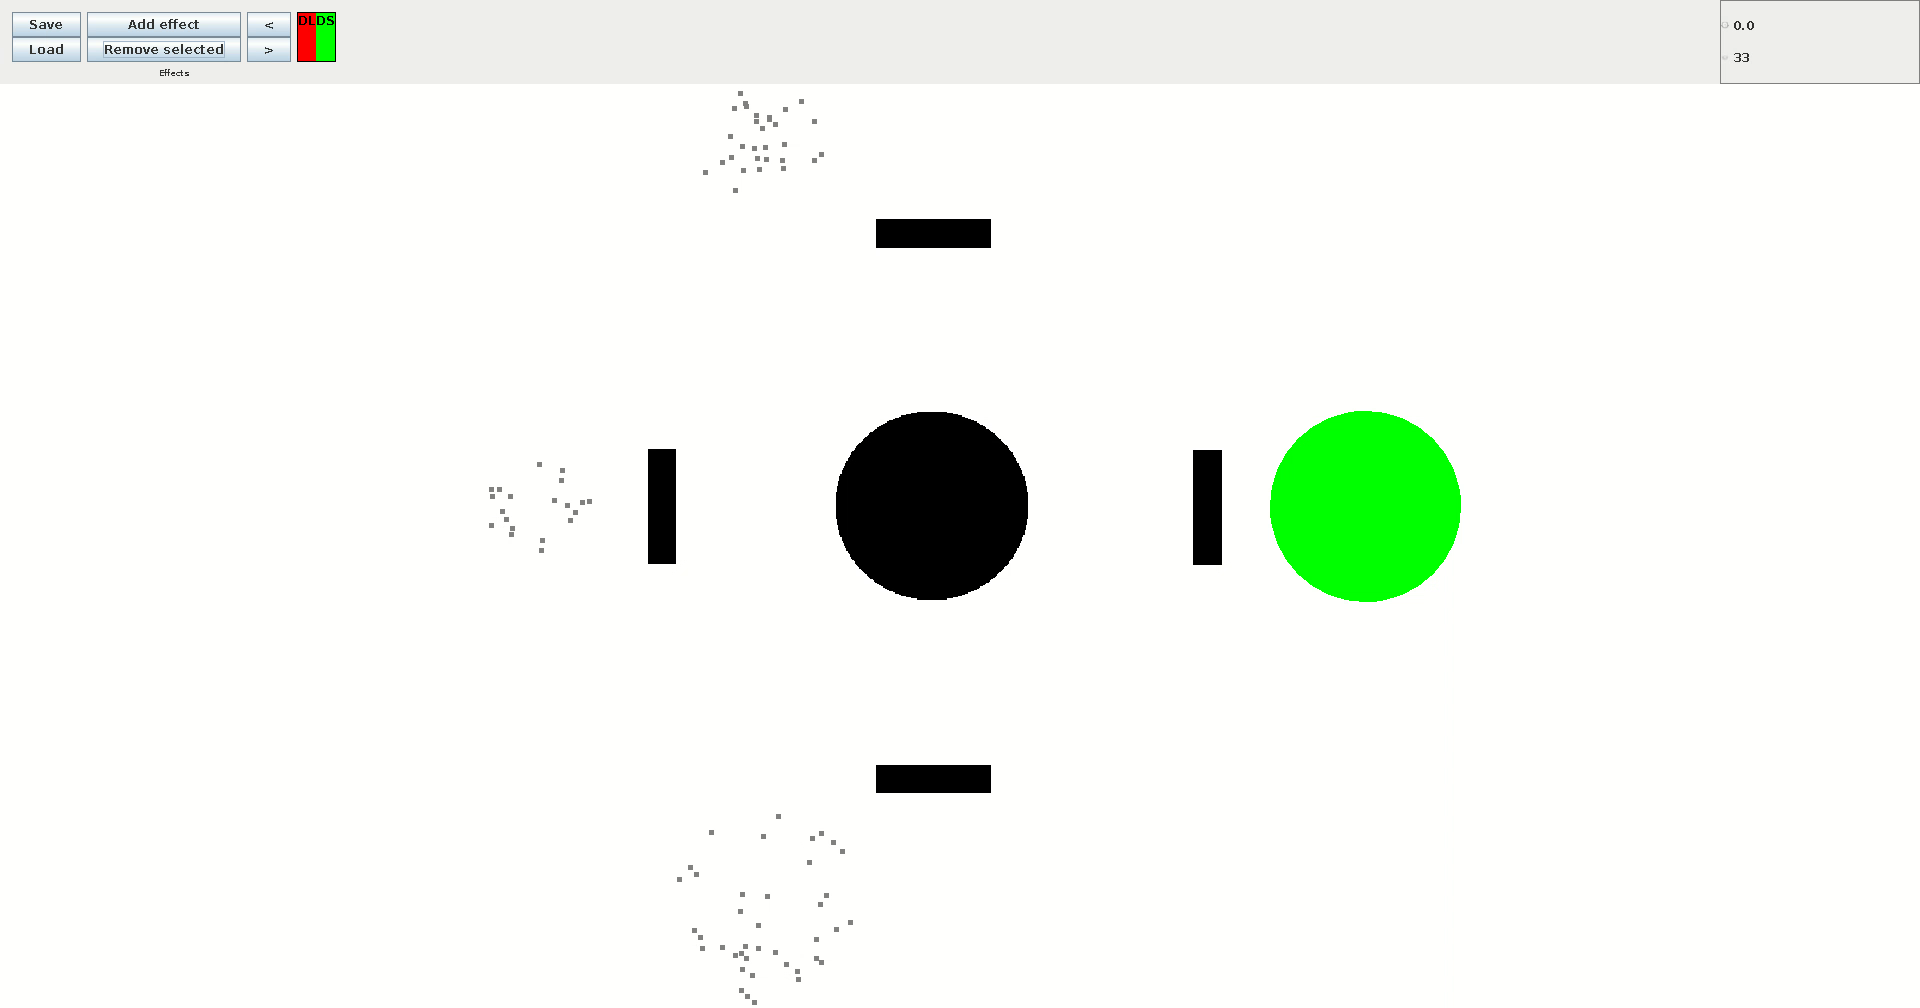
\includegraphics[width=\textwidth]{immagini/casi-studio/no-obstacle-avoidance-begin.png}
    \end{subfigure}
    \hfill
    \begin{subfigure}[b]{0.75\textwidth}
        \centering
        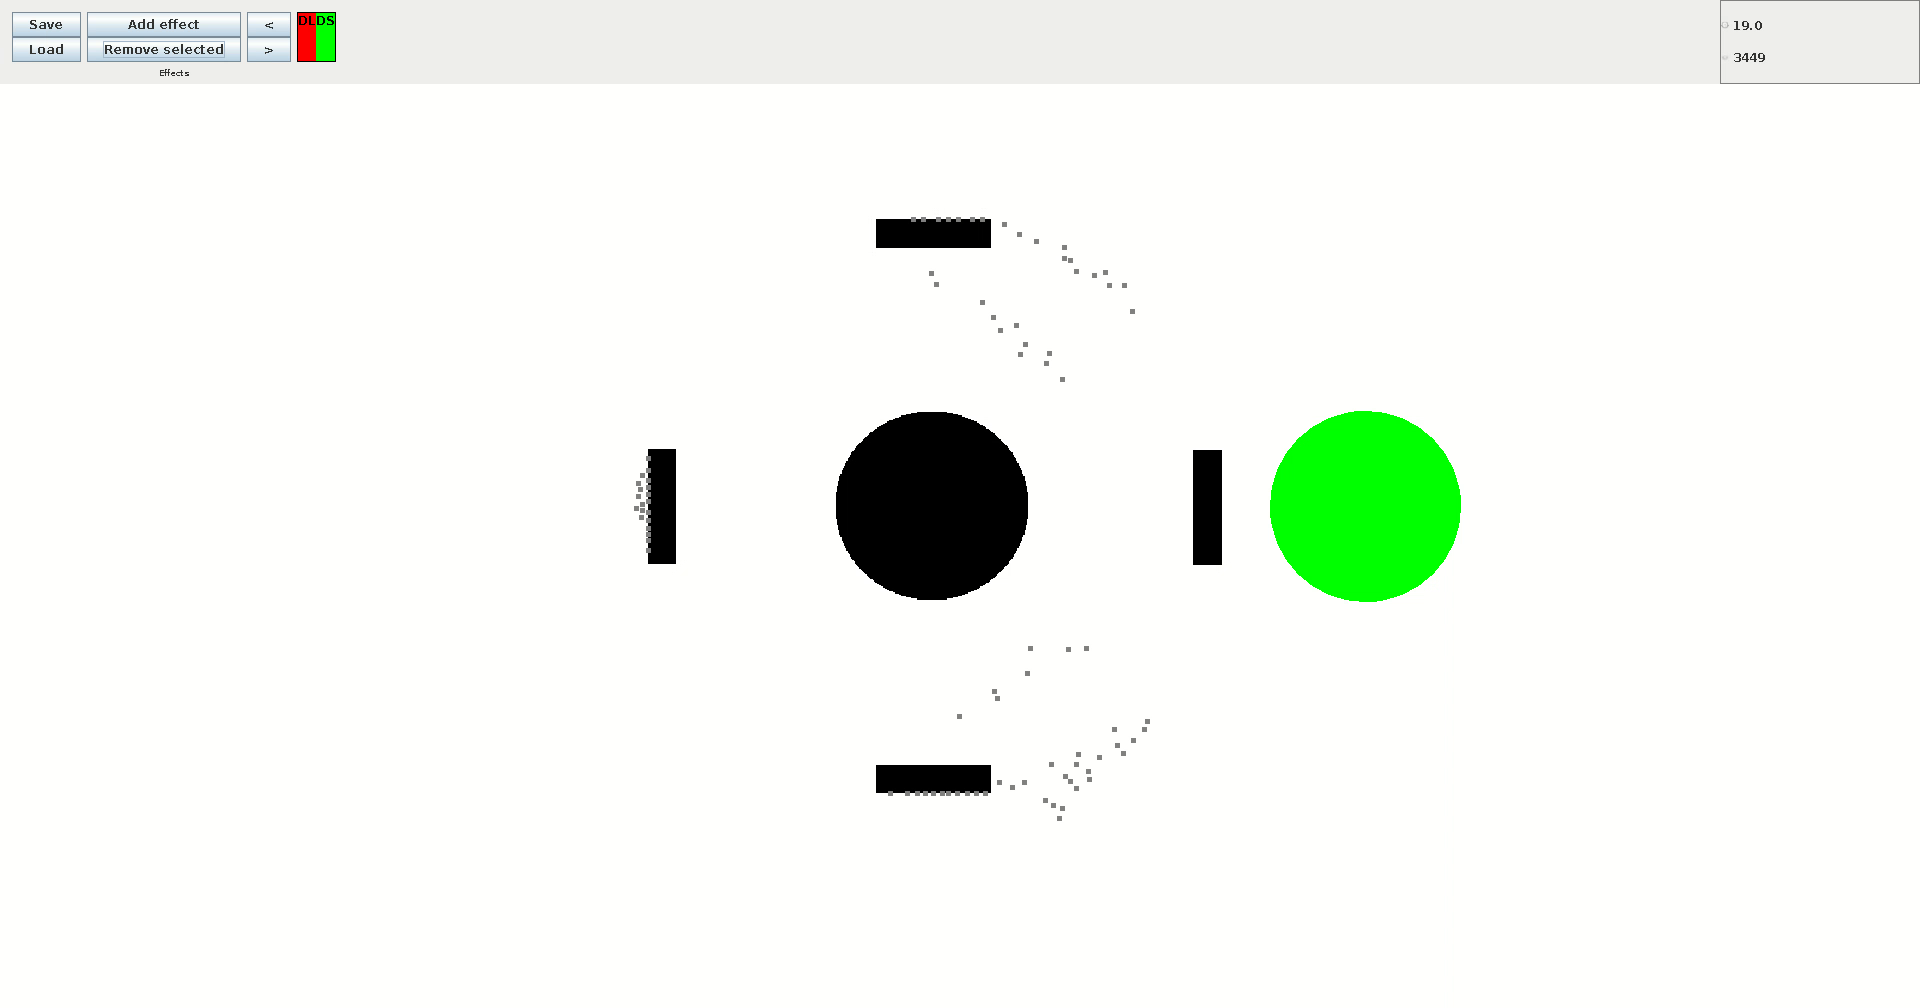
\includegraphics[width=\textwidth]{immagini/casi-studio/no-obstacle-avoidance-during.png}
    \end{subfigure}
    \hfill
    \begin{subfigure}[b]{0.75\textwidth}
        \centering
        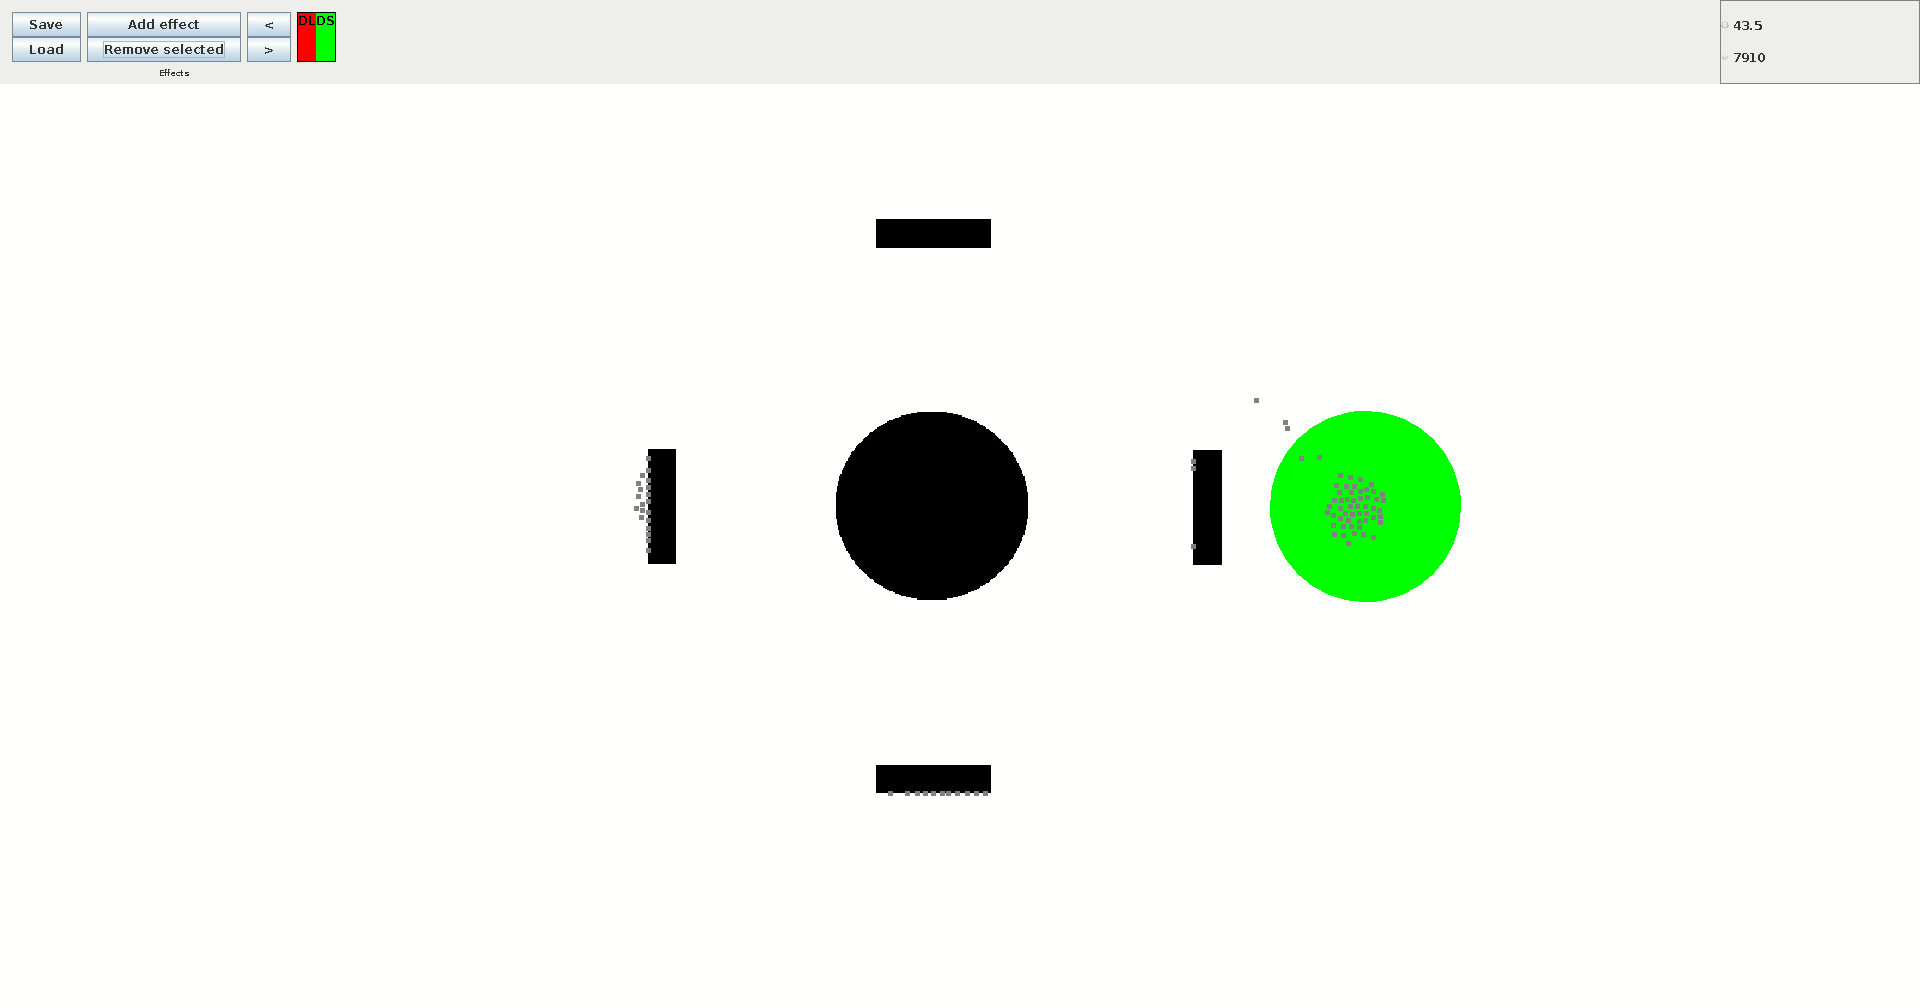
\includegraphics[width=\textwidth]{immagini/casi-studio/no-obstacle-avoidance-end.png}
    \end{subfigure}
    \caption{Fotogrammi salienti della simulazione in cui sono presenti ostacoli non considerando il comportamento di steering ad essi associato; molti pedoni rimangono bloccati durante il loro percorso e non riescono a raggiungere la zona di sicurezza.}
    \label{fig:no-obstacle-avoidance}
\end{figure}

\begin{figure}
    \centering
    \begin{subfigure}[b]{0.75\textwidth}
        \centering
        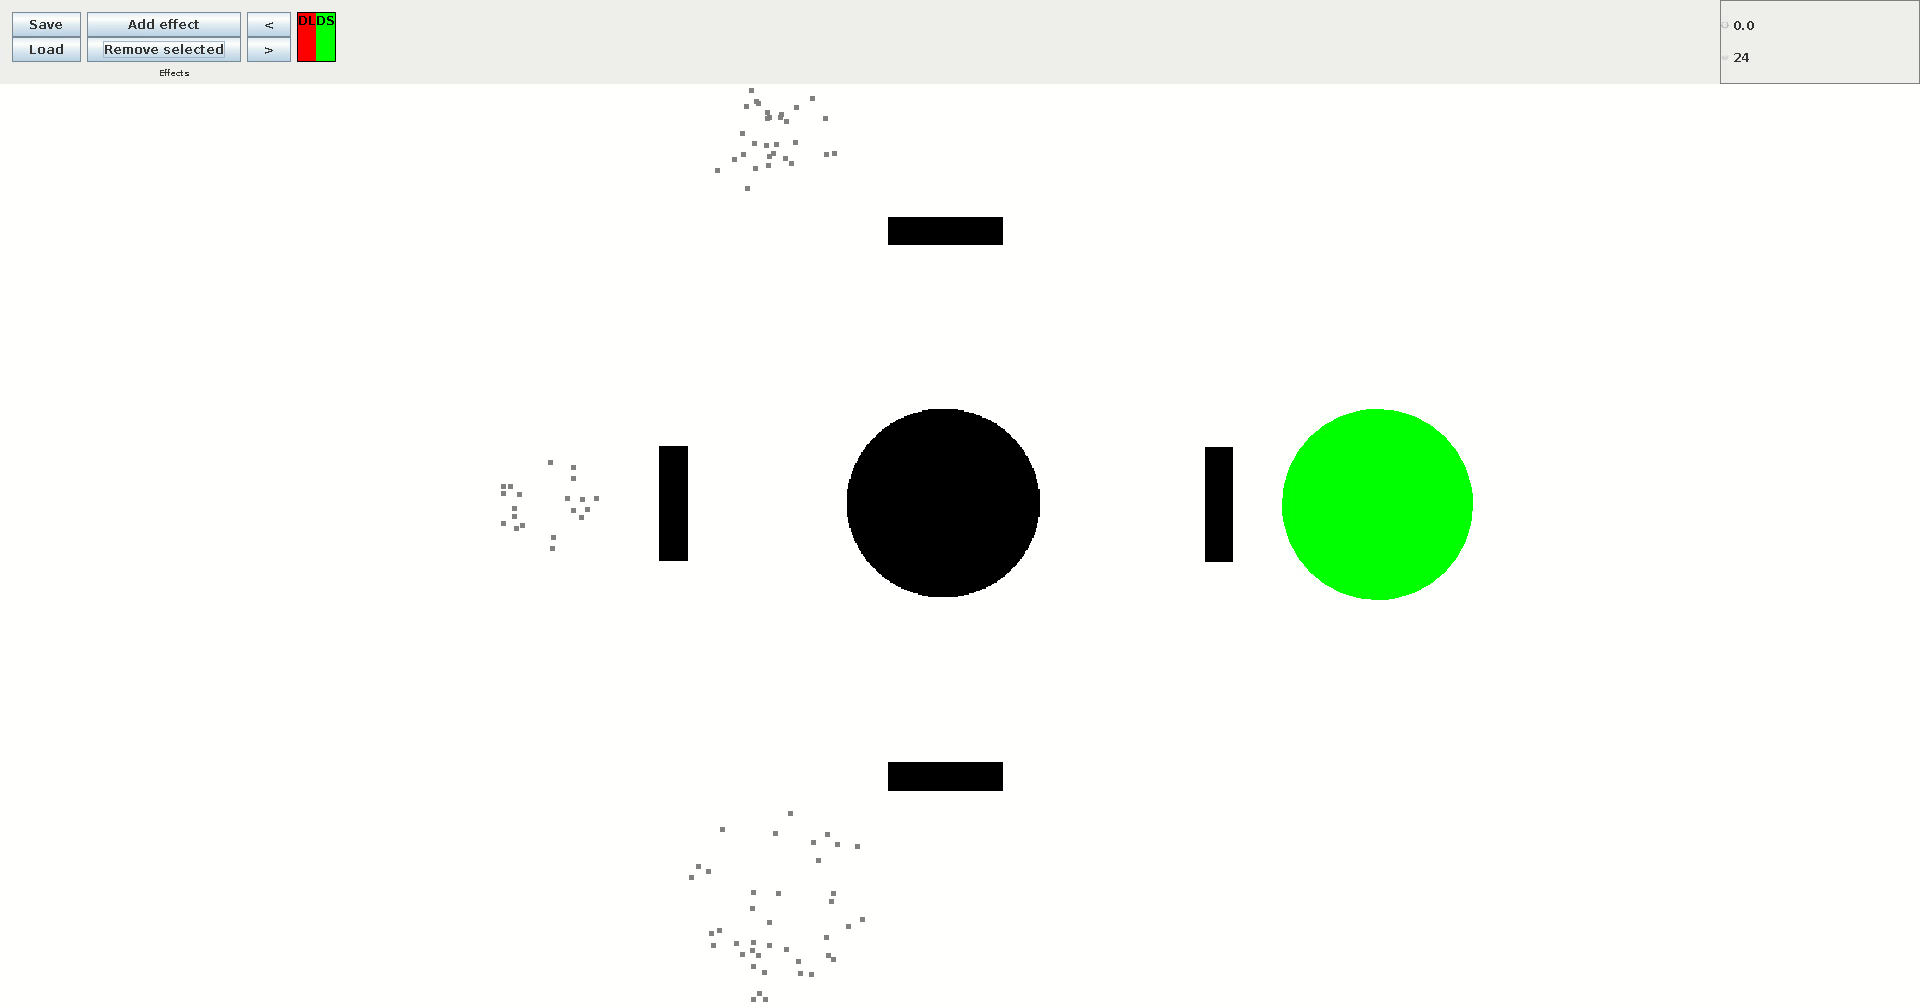
\includegraphics[width=\textwidth]{immagini/casi-studio/obstacle-avoidance-begin.png}
    \end{subfigure}
    \hfill
    \begin{subfigure}[b]{0.75\textwidth}
        \centering
        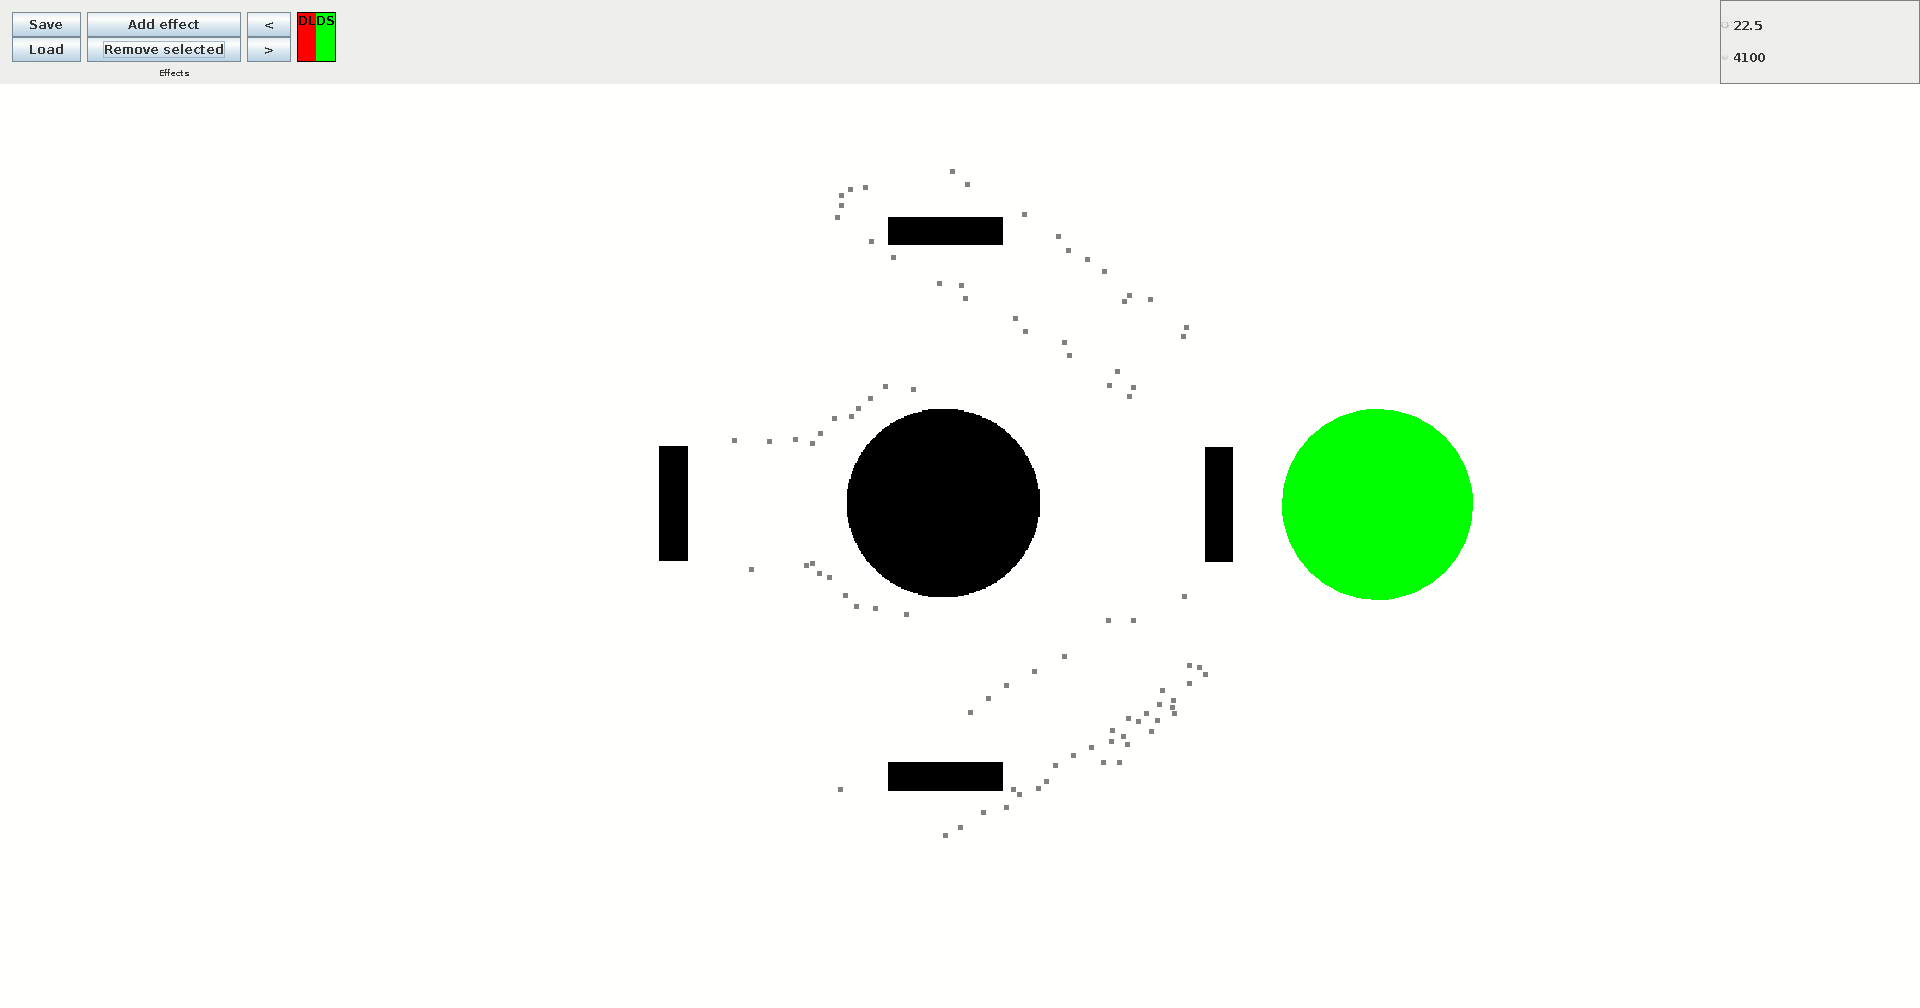
\includegraphics[width=\textwidth]{immagini/casi-studio/obstacle-avoidance-during.png}
    \end{subfigure}
    \hfill
    \begin{subfigure}[b]{0.75\textwidth}
        \centering
        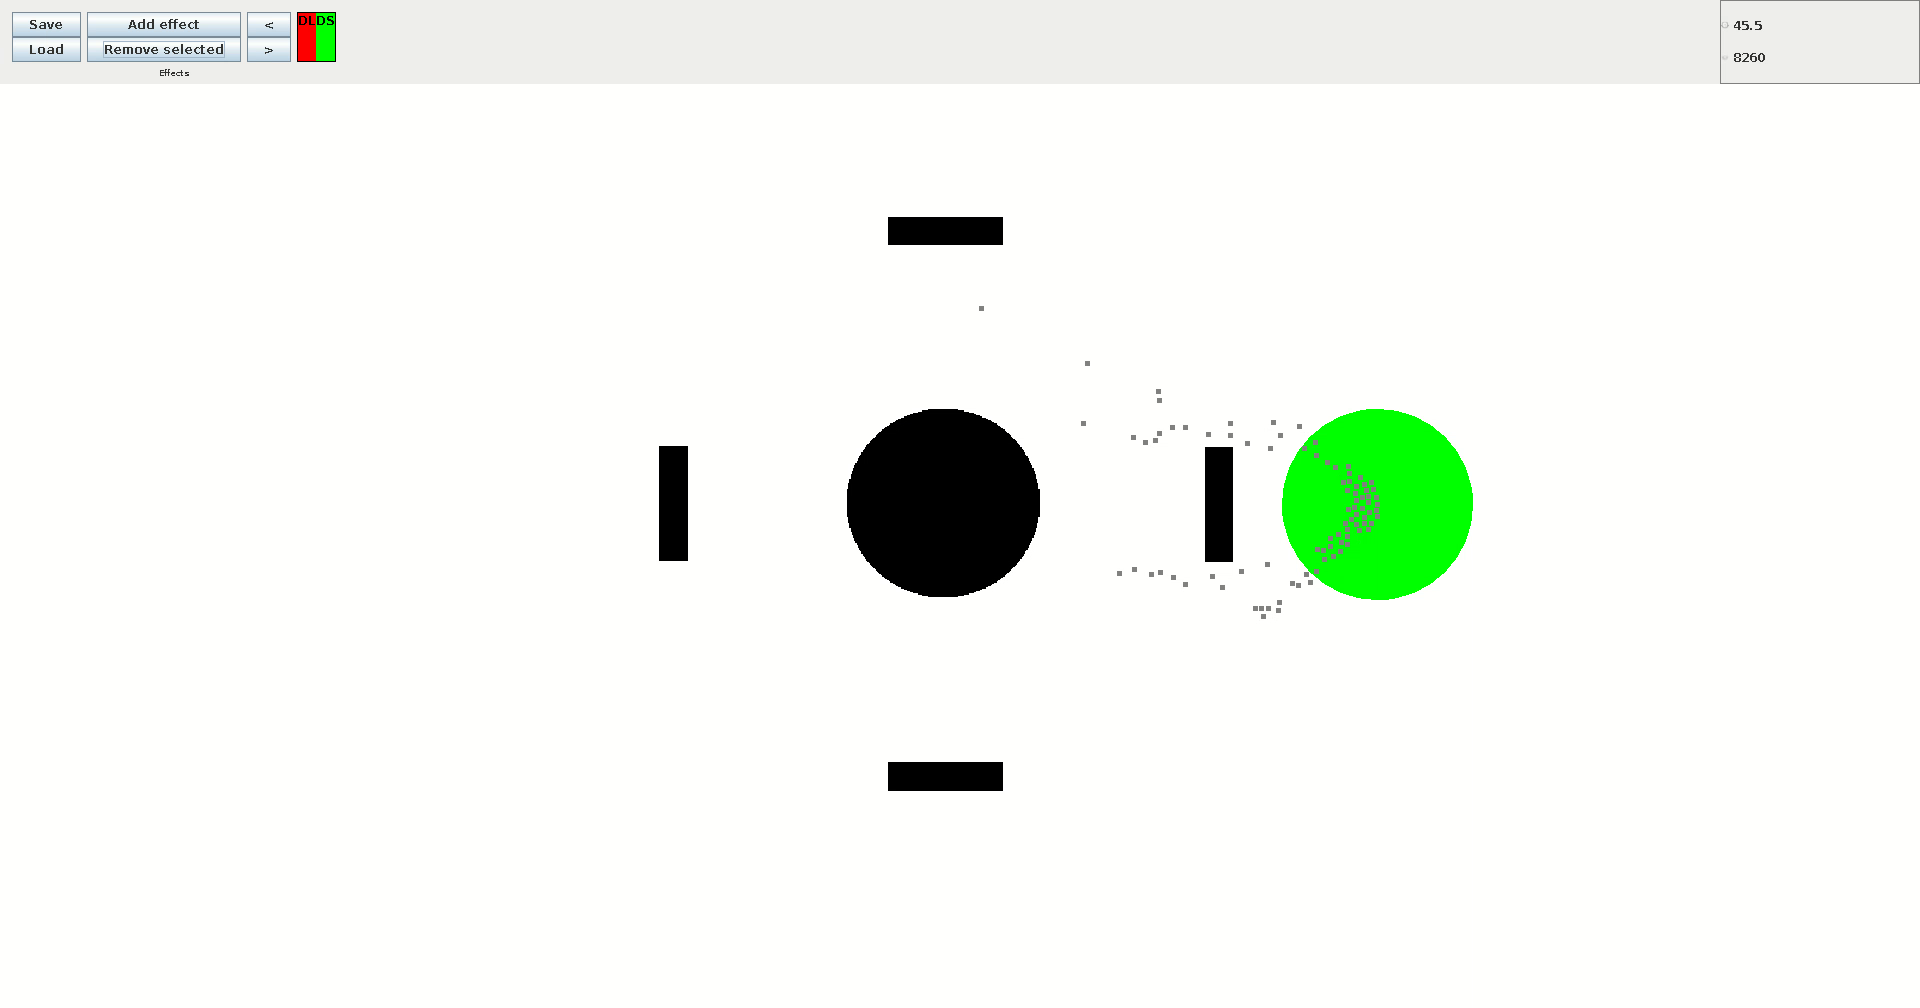
\includegraphics[width=\textwidth]{immagini/casi-studio/obstacle-avoidance-end.png}
    \end{subfigure}
    \caption{Fotogrammi salienti della simulazione in cui sono presenti ostacoli considerando il comportamento di steering ad essi associato; tutti i pedoni riescono a raggiungere la zona di sicurezza evitando eventuali oggetti presenti sul loro cammino.}
    \label{fig:obstacle-avoidance}
\end{figure}
\page{empty}

\chapter{Conclusioni e sviluppi futuri}
\section{Conclusioni}
Traendo ispirazione dalle idee presentate nel modello IMPACT, le caratteristiche inerenti un agente sono state rielaborate ed introdotte all'interno del simulatore Alchemist, differenziando sulla base di esse tre tipologie di pedone: omogeneo, eterogeneo, continuo. L'utilizzo di questo approccio permette la scelta del livello di dettaglio che si ritiene più opportuno per rappresentare i protagonisti della simulazione. \newline
Al fine di riprodurre i movimenti umani si è optato per l'uso dei comportamenti di steering trattati da Reynolds, forze determinate da scelte localizzate che, se unite tra loro, possono rappresentare dinamiche complesse. Non esistendo una regola generale per combinare questi atteggiamenti, sono state formulate varie strategie per poter rispondere alle diverse esigenze che uno specifico scenario o una particolare situazione possono richiedere. \newline
Data la frequente presenza di gruppi di persone (famiglie, coppie, amici) rispetto a quella di individui solitari, anche questo concetto e le relative dinamiche sono state inclusi nella modellazione degli agenti. \newline
Nonostante la metodologia utilizzata sia principalmente basata sul modello ad agenti, sono stati adottati anche aspetti caratteristici degli automi cellulari e delle forze sociali, in accordo con il suggerimento di Zheng di utilizzare insieme più approcci per sfruttare al meglio i vantaggi di ognuno di essi \cite{Zheng2009}. \newline
L'uso del paradigma orientato agli oggetti e di un linguaggio all'avanguardia come Kotlin, garantiscono delle solide basi per poter ampliare questo lavoro, raffinandolo o estendendolo con altre funzionalità. La natura agnostica all'incarnazione utilizzata, su cui è incentrata la progettazione, permette ampia libertà di scelta su come sfruttare le nuove potenzialità offerte. \newline
Per dimostrare gli effetti dei diversi fattori considerati per modellare i pedoni, sono state eseguite delle simulazioni significative, valutate sia in assenza che in presenza del fenomeno in esame e poi confrontate. Differenze cospicue tra le due versioni sono state riscontrate in tutti gli scenari e i risultati denotano macroscopicamente delle attitudini che, in accordo con le ricerche basate su osservazioni empiriche citate, rispecchiano quelle che le controparti umane degli agenti avrebbero in natura. \newline
A fronte di questi contributi, il simulatore Alchemist possiede i principali elementi necessari a riprodurre l'evacuazione di una folla in svariate situazioni. Ancora la maturità necessaria a poter descrivere esaustivamente circostanze che, per la struttura dell'ambiente in cui sono analizzate o l'ingente numero di aspetti valutati contemporaneamente, si rivelano troppo complesse non è stata raggiunta, ma i primi passi per perseguirla sono stati mossi.
\section{Sviluppi futuri}
Per migliorare il supporto di Alchemist al problema della simulazione del comportamento delle folle, vengono fornite delle direzioni di ricerca verso le quali il lavoro qui presentato può essere esteso.

\paragraph{Forma dei pedoni}
Attualmente i pedoni vengono tutti rappresentati mediante dei cerchi di dimensione predefinita. Alla stregua di altre caratteristiche come la velocità, il sesso o l'età, anche la forma dovrebbe essere eterogenea, in modo da ricalcare più fedelmente l'occupazione reale dell'agente nello spazio. \newline
Per questo motivo, è necessario definire sia diverse dimensioni in relazione all'età e al sesso del pedone sia delineare la corporatura con delle forme geometriche più simili a quelle che questa presenta in natura. Due possibili alternative per quest'ultimo aspetto, menzionate da Chen nell'analisi delle varie versioni esistenti del modello forze sociali \cite{Chen2017}, sono l'ellisse e la rappresentazione \enquote{tre cerchi}, due dei quali costituiscono le spalle mentre quello al centro la testa.

\paragraph{Ruolo dei pedoni}
Le simulazioni che sono state discusse, vedono come protagonisti pedoni che hanno tutti una conoscenza limitata al loro intorno e a quello che vedono dell'ambiente circostante. \newline 
In realtà, potrebbero esistere anche degli agenti che hanno più familiarità di altri con l'ambiente in cui sono inseriti e
quindi, per muoversi all'interno di esso potrebbero far uso di strategie di esplorazione globale come l'\textit{algoritmo di Dijkstra} o $A^{*}$. \newline 
Un esempio di questa differenziazione è fornito in \cite{Tan2019} dalle tipologie \textit{visitor} e \textit{tenant} e può essere usato come punto di partenza per analizzare questo tema.

\paragraph{Collisioni realistiche}
L'introduzione di ambienti caratterizzati da una componente fisica, per ora, impedisce ad un nodo di andare ad occupare una posizione in cui ne è già presente un altro ma non gestisce le forze in gioco in una potenziale collisione tra essi, che viene solamente prevenuta impedendo lo spostamento. \newline
Una zona ad alta densità, è contraddistinta da una quantità enorme di questi urti scaturiti dal movimento frenetico dei pedoni quindi, riuscire a riprodurli, porterebbe degli importanti miglioramenti per il realismo della simulazione.

\paragraph{Relazioni tra gruppi}
Un gruppo, analogamente ad un pedone, può essere considerato come un’agente della simulazione e, in quanto tale, potrebbe essere influenzato o influire sulle scelte degli altri gruppi presenti nell'ambiente. \newline
Queste possibilità vengono analizzate da Qiu e Xu in \cite{Qiu2010}, dove ad ogni gruppo viene associata una matrice intra-relazionale per definire i rapporti tra ogni possibile coppia di pedoni al suo interno e vi è un’unica matrice inter-relazionale per evidenziare l’influenza reciproca dei diversi gruppi presenti. \newline
Grazie a questa modellazione, non solo è possibile differenziare le attitudini delle varie tipologie di gruppo, ma è anche pensabile delineare la struttura che i vari membri o i vari gruppi devono assumere durante il movimento.

\paragraph{Differenze culturali}
Le caratteristiche di un pedone non sono solo biologiche, mentali o strutturali ma possono avere influssi derivanti anche dalla sua cultura. \newline
La storia, le abitudini e l'ideologia di un paese sono indubbiamente fattori che incidono sul modo di agire di un agente che vive al suo interno e perciò vanno studiati per i diversi popoli esistenti e inclusi nei modelli di evacuazione. \newline
Per avere un'idea più chiara di come inserire questi aspetti in un modello ad agenti, si può partire dal contributo basato su osservazioni empiriche descritto in \cite{Fridman2013}.
\page{empty}

\printbibliography
\page{empty}

% Ringraziamenti
\chapter*{Ringraziamenti}
\addcontentsline{toc}{chapter}{Ringraziamenti}
Giunto al termine di questo percorso di studi, mi scopro una persona completamente diversa rispetto a quando ho iniziato. Questo corso mi ha dato tanto sia in termini di conoscenze acquisite sia di rapporti umani con coloro con cui ho collaborato e mi sono confrontato. \newline 
Ancora non è tempo di fermarmi, per poter provare ad utilizzare le potenzialità offerte dal mondo dell'informatica per risolvere gli svariati problemi che affliggono la nostra società, ho bisogno di continuare a studiare e mettermi alla prova. \newline 
Questo lavoro di tesi rappresenta il primo passo verso la direzione che mi sono prefissato, ma anche l'ultimo di un viaggio fantastico iniziato tre anni fa e di cui non rimpiango nessuna scelta. \newline
Se oggi posso essere fiero di dove sono arrivato, lo devo a tutti coloro che mi hanno supportato e accompagnato in questa esperienza e senza i quali molto probabilmente tutto questo non sarebbe stato realizzabile. \newline
La prima menzione va alla mia famiglia: a mio padre Giuliano, a mia madre Maria e a mia sorella Sofia, le persone che considero più importanti, che si sono sempre fidate di me e sono rimaste al mio fianco anche a più di 100km di distanza. Insieme a loro non posso non nominare i miei zii Umberto e Silvana e i miei cugini Mauro, Claudia, Nicoletta e Mikael, amici prima ancora di parenti e vicini di casa. \newline
Parlando di amici, un trattamento speciale va riservato a Luca e Milo, con i quali ho condiviso l'appartamento, l'università e la maggior parte della mia storia a Cesena, che però non sarebbe stata la stessa senza aver conosciuto Pierdomenico, Filippo, Augusto, Diego, Martina, Benedetta, Chiara, Beatrice e Sofia, quest'ultima solo ora menzionata perché mi sono dimenticato di inserirla tra i coinquilini. \newline
Oltre a loro, ci sono ovviamente anche gli amici che ho lasciato a Jesi quando sono partito per Cesena, che mi vedo costretto a citare con il rispettivo nickname non avendo ormai memoria dell'ultima volta che li ho chiamati con il loro nome di battesimo. Quindi grazie anche a voi Silver, Ferro, Fabri Piglia e Sax. \newline
Volevo concludere ringraziando tutti i professori del corso di studi in Ingegneria e Scienze informatiche, in particolare il professor Pianini ed il professor Viroli, che mi hanno seguito ed aiutato durante il tirocinio prima ed in questo progetto di tesi poi.
\page{empty}

% Appendice
\appendix
\chapter{File di simulazione}
\section{Influenza del gruppo}

\begin{minted}[gobble=0,frame=single,linenos]{yaml}
incarnation: protelis

environment:
  type: Continuous2DEnvironment

seeds:
  scenario: 0
  simulation: 1

variables:
  group1: &group1
    formula: it.unibo.alchemist.model.implementations.groups.Friends<Any>()
    language: kotlin
  group2: &group2
    formula: it.unibo.alchemist.model.implementations.groups.Friends<Any>()
    language: kotlin
  group3: &group3
    formula: it.unibo.alchemist.model.implementations.groups.Friends<Any>()
    language: kotlin
  group4: &group4
    formula: it.unibo.alchemist.model.implementations.groups.Friends<Any>()
    language: kotlin
  danger: &danger
    formula: "\"danger\""

layers:
  - type: BidimensionalGaussianLayer
    molecule: *danger
    parameters: [0.0, 0.0, 1.0, 2.0]

reactions: &behavior
  - time-distribution:
      type: DiracComb
      parameters: [2.0]
    type: BlendedSteering
    actions:
      - type: Cohesion
      - type: AvoidFlowField
        parameters: [*danger]

displacements:
  - in:
      type: Circle
      parameters: [8, 0, 0, 15]
    nodes:
      type: HomogeneousPedestrian2D
      parameters: [*group1]
    programs:
      - *behavior
  - in:
      type: Circle
      parameters: [4, 0, 0, 15]
    nodes:
      type: HomogeneousPedestrian2D
      parameters: [*group2]
    programs:
      - *behavior
  - in:
      type: Circle
      parameters: [10, 0, 0, 15]
    nodes:
      type: HomogeneousPedestrian2D
      parameters: [*group3]
    programs:
      - *behavior
  - in:
      type: Circle
      parameters: [2, 0, 0, 15]
    nodes:
      type: HomogeneousPedestrian2D
      parameters: [*group4]
    programs:
      - *behavior
\end{minted}

\section{Contagio sociale}

\begin{minted}[gobble=0,frame=single,linenos]{yaml}
incarnation: protelis

variables:
  danger: &danger
    formula: "\"danger\""
  target: &target
    formula: "\"target\""

environment:
  type: Continuous2DEnvironment

layers:
  - type: BidimensionalGaussianLayer
    molecule: *danger
    parameters: [80, 0, 100, 15]
  - type: BidimensionalGaussianLayer
    molecule: *target
    parameters: [-50, 0, 10, 5]

seeds:
  scenario: 0
  simulation: 1

steering: &steering
  - time-distribution:
      type: DiracComb
      parameters: [2.0]
    type: PrioritySteering
    actions:
      - type: AvoidFlowField
        parameters: [*danger]
      - type: FollowFlowField
        parameters: [*target]
    conditions:
      - type: WantToEvacuate
        parameters: [*danger]

cognitive: &cognitive
  - time-distribution:
      type: DiracComb
      parameters: [0.5]
    type: CognitiveBehavior
    actions:
      - type: RandomRotate

displacements:
  - in:
      type: Circle
      parameters: [25, 0, 0, 8]
    nodes:
      type: CognitivePedestrian2D
      parameters: ["adult", "female", *danger]
    programs:
      - *steering
      - *cognitive
  - in:
      type: Circle
      parameters: [75, 60, 0, 10]
    nodes:
      type: CognitivePedestrian2D
      parameters: ["adult", "male", *danger]
    programs:
      - *steering
      - *cognitive
\end{minted}

\section{Scelta dell'uscita}

\begin{minted}[gobble=0,frame=single,linenos]{yaml}
incarnation: protelis

variables:
  danger: &danger
    formula: "\"danger\""
  exit1: &exit1
    formula: "\"exit1\""
  exit2: &exit2
    formula: "\"exit2\""
  exit3: &exit3
    formula: "\"exit3\""
  exit4: &exit4
    formula: "\"exit4\""

environment:
  type: ImageEnvironment
  parameters: [images/multiple-exits.png, 0.0416]

seeds:
  scenario: 1
  simulation: 0

layers:
  - type: BidimensionalGaussianLayer
    molecule: *danger
    parameters: [10, 10, 100, 3]
  - type: BidimensionalGaussianLayer
    molecule: *exit1
    parameters: [0, 0, 10, 50, 0.5, 0.5]
  - type: BidimensionalGaussianLayer
    molecule: *exit2
    parameters: [0, 10, 20, 50, 0.5, 0.5]
  - type: BidimensionalGaussianLayer
    molecule: *exit3
    parameters: [0, 20, 10, 50, 0.5, 0.5]
  - type: BidimensionalGaussianLayer
    molecule: *exit4
    parameters: [0, 10, 0, 50, 0.5, 0.5]

reactions: &behavior
  - time-distribution:
      type: DiracComb
      parameters: [1.0]
    type: BlendedSteering
    conditions:
      - type: WantToEvacuate
        parameters: [*danger]
    actions:
      - type: AvoidFlowField
        parameters: [*danger]
      - type: FollowFlowField
        parameters: [*exit1]
      - type: FollowFlowField
        parameters: [*exit2]
      - type: FollowFlowField
        parameters: [*exit3]
      - type: FollowFlowField
        parameters: [*exit4]
  - time-distribution:
      type: DiracComb
      parameters: [0.25]
    type: CognitiveBehavior
    actions:
      - type: RandomRotate

displacements:
  - in:
      type: Circle
      parameters: [75, 10, 10, 8]
    nodes:
      type: CognitivePedestrian2D
      parameters: ["adult", "male", *danger]
    programs:
      - *behavior
  - in:
      type: Circle
      parameters: [75, 10, 10, 8]
    nodes:
      type: CognitivePedestrian2D
      parameters: ["adult", "female", *danger]
    programs:
      - *behavior
\end{minted}

\section{Presenza di ostacoli}

\begin{minted}[gobble=0,frame=single,linenos]{yaml}
incarnation: protelis

variables:
  target: &target
    formula: "\"target\""

environment:
  type: ImageEnvironment
  parameters: [images/obstacles.png, 0.125]

seeds:
  scenario: 0
  simulation: 1

layers:
  - type: BidimensionalGaussianLayer
    molecule: *target
    parameters: [75.0, 30.0, 20.0, 10.0]

reactions: &behavior
  - time-distribution:
      type: DiracComb
      parameters: [2.0]
    type: BlendedSteering
    actions:
      - type: FollowFlowField
        parameters: [*target]
      - type: ObstacleAvoidance
        parameters: [6]

displacements:
  - in:
      type: Circle
      parameters: [20, -12, 30, 5]
    nodes:
      type: HomogeneousPedestrian2D
    programs:
      - *behavior
  - in:
      type: Circle
      parameters: [30, 12, 68, 7]
    nodes:
      type: HomogeneousPedestrian2D
    programs:
      - *behavior
  - in:
      type: Circle
      parameters: [40, 12, -12, 10]
    nodes:
      type: HomogeneousPedestrian2D
    programs:
      - *behavior
\end{minted}

\end{document}